\documentclass[a4paper,11pt]{report}

\usepackage[english, polish]{babel}
\usepackage[utf8]{inputenc}
\usepackage{blindtext}
\usepackage[T1]{fontenc}
\usepackage{booktabs}
\usepackage{float}
\usepackage{graphicx}
\usepackage{wrapfig}
\usepackage{caption}
\usepackage{multirow}
\usepackage[export]{adjustbox}
\usepackage[nottoc,notlot,notlof]{tocbibind}

\graphicspath{ {./images/} }

\begin{document}
\let\cleardoublepage\clearpage
\begin{figure}[ht]
\centering

\includegraphics{pjatk}
\end{figure}
\begin{center}
\textbf{\huge Karta Projektu}\\
\vspace{1cm}
\begin{tabular}{|p{15cm}|}
\hline
\textbf{Temat projektu:}\\Gamitude manage your Energy, not your Time\\ 
\hline
\textbf{Akronim:}\\GTM\\
\hline
\textbf{Opiekun:}\\Tadeusz Puźniakowski  \\
\hline
\textbf{Konsultanci:}\\Tadeusz Puźniakowski\\Marek Bednarczyk \\
\hline
\textbf{Cele projektu:}
\\Dostarczenie użytkownikom narzędzia do zarządzania ich energią,
 opartego o najnowsze odkrycia dotyczące ludzkiej produktywności.
Jednocześnie chcemy,
 aby użytkownicy zaczęli postrzegać prace bądź naukę bardziej pozytywnie dzięki powiązaniom pracy z elementami gier RPG.\\
\hline
\textbf{Rezultaty projektu:}\\Kompletny system do zarządzania projektami opierający się na najnowszych badaniach dotyczących ludzkiej produktywności. \\
\hline
\textbf{Miary sukcesu:}\\Działający system projektów, Bullet Journal, Gamitude Themes.\\
\hline
\textbf{Ograniczenia:}\\Czasowe, umiejętnościowe, budżetowe \\
\hline
\end{tabular}\\
\vspace{1cm}
\begin{tabular}{|l|l|l|l|}
\hline
\textbf{Wykonawca} & \textbf{Numer albumu}& \textbf{Specjalizacja}& \textbf{Tryb studiów} \\
\hline
Robert Deyk&s17707&SI&Stacjonarne \\
\hline
Paweł Benkowski&s16569&SI&Stacjonarne\\
\hline
Stanisław Lutkiewicz&s17535&SI&Stacjonarne \\
\hline
\end{tabular}\\
\vspace{1cm}
\begin{tabular}{|l|l|l|l|}
\hline
\textbf{Data ukończenia projektu:} & to be determined & \textbf{Recenzent:} & to be determined\\
\hline
\end{tabular}
\end{center}
\tableofcontents

\chapter{Wprowadzenie}
\subsubsection{Kontekst pracy}
Energie\cite{Harward} dzielą się na 4 rodzaje: duszy, ciała, emocji i umysłu.
\\Istnieją różne techniki próbujące wspomóc ich efektywne wykorzystywanie jak metoda Pomodoro\cite{Pomodoro} czy Ultradian Rhythm\cite{90/30}.
\\\\Pierwsza technika polega na dzieleniu czasu pracy na 25-minutowe sesje, po których następuje 5-minutowa przerwa.
 Po wykonaniu 5 takich sesji przerwa wydłuża się do 15 minut.
 Technika ta jest szczególnie przydatna podczas nauki.
\\Jak wiadomo z badań, po nauce należy dać mózgowi czas na 'przetworzenie' nowych informacji.
 Tworzy on w tym czasie nowe synapsy, dołączając nowo nabytą wiedze do istniejącej sieci informacji.
 Jeżeli napotka terminy podobne do nowej informacji, połączy je,  umacniając strukturę. 
\\\\Druga technika polega na dzieleniu czasu na pracy na 90-minutowe sesje, po których następuje 30-minutowa przerwa.
 Technika ta jest oparta na naturalnym cyklu ludzkiej aktywności podczas dnia.
 Ultradian Rhythm jest szczególnie przydatny przy zadaniach rutynowych bądź częściowo rutynowych.
 Przykładem takiego zadania jest praca.
\\\\Są to tylko dwie najpopularniejsze metodyki pracy, dzięki którym zwiększamy swoją wydajność. 
Na bierząco śledzimy literaturę fachową z tego obszaru w celu znalezienia nowych technik,
 tak aby Gamitude oferował, jak najszersze możliwości personalizacji. 
\\\\Niekiedy jednak projekty trzeba rozplanować jako zadania w kontekście czasu.
 Na takie okazje stworzyliśmy Bullet Journal\cite{bulletJournal}.
 Jest to dziennik ze stronami dedykowanymi na zadania z określonym terminem wykonania tj. dzisiaj, tydzień lub miesiąc bądź w nieokreślonej przyszłości.
\\\\Aby użytkownik czuł, że jego praca przynosi efekty, dodaliśmy również elementy grywalizacji\cite{grywalizacja}, czyli 
 statystyki oraz rangi\cite{rangi}, gdzie statystyki można rozumieć jako sztuczną walutę podzieloną na 4 rodzaje a rangi 
 jako awatara użytkownika kupowanego za te waluty.
\subsubsection{Przedstawienie problemu}
Według pracy harwardzkiej\cite{Harward}, ludzie organizujący sobie prace, mają tendencje do siadania i wykonywania jej bez przerwy aż do ukończenia,
 ignorując holistyczną naturę działania ludzkiego organizmu oraz naturalne cykle zachodzące w ludzkim ciele.
 W pracy czas jest porównywany do węgla a energia do wiatru.
 Jest to nawiązanie do przemysłu energetycznego i cech źródeł odnawialnych i nieodnawialnych.

\subsubsection{Cel i zakres projektu}
Celem jest stworzenie systemu, który swoje działanie bazuje na energiach omówionych wcześniej,
 zwracając także uwagę na nie przepracowywanie użytkowników.\\
Zakresem projektu jest stworzenie zestawu narzędzi szanujących higienę pracy
 oraz indywidualne preferencje organizacji pracy przez użytkowników.

\subsubsection{Podejście do projektu}
Zwinne, Scrumban, aplikacja webowa oparta o jezyk skryptowy JavaScript, backend napisany w języku .NET Core, wybrane ze względu na wieloplatformowość.

\subsubsection{Rezultaty}
Ludzie potrafią utrzymać produktywność w dłuższym okresie, bez ubytków w żadnej z dziedzin życia.

\subsubsection{Organizacja dokumentu}
Omówienie problemu, analiza projektu, projektowanie i implementacja systemu, historia implementacji,
 testy systemu, testy w grupie docelowej, nakład pracy, wkład własny, podsumowanie

\section {Słownik pojęć}
	\emph{Bullet Journal – dziennik, w którym można rozplanowywać bardziej skomplikowane zadania na mniejsze}\\
	\emph{Czasomierz — komponent odpowiedzialny za odliczanie czasu, może przybrać postać minutnika, stopera i skomplikowanego minutnika}\\
	\emph{Dzienniki — zbiór stron zawierające zadania}\\
	\emph{Elastic Habits – stopniowanie zadania na 3 poziomy}\\
	\emph{Energie — Liczbowa reprezentacja zasobów, które użytkownik może wykożystać do wykonywania projektów}\\
	\emph{Foldery — katalogi przetrzymujące projekty}\\
	\emph{Statystyki — Liczbowa reprezentacja poświęconego czasu nad projektami}\\
	\emph{Memoizacja — zapisywanie wyników działania obliczeniowo ciężkich funkcji do ponownego wykorzystania}\\
	\emph{Motywy — szata kolorystyczna aplikacji możliwa do zmiany}\\
	\emph{Projekt – Czynność bądź umiejętność, nad którą użytkownik chce pracować, nie ma podziału na podpunkty, skupiający się na czasie}\\
	\emph{Rangi — Grafiki kupowane przez użytkownika za pomocą statystyk}\\
	\emph{Statystyka dominująca — statystyka, która jest najbardziej rozwijana przez projekt}\\
	\emph{Strony — strony dziennika zawierające zadania do wykonania}\\
	\emph{Tier — poziom rzadkości rangi}\\
	\emph{Wzmacniane statystyki — statystyki wzmacniane przez projekt}\\
	\emph{Zadania — pomniejsze rzeczy do wykonania}\\
	

\chapter {Omówienie problemu}
\section {Przedstawienie problemu}
\subsubsection{Problem a ludzie}
Problemem jest utrzymanie produktywności bez ubytku w innych sferach życia np. życia rodzinnego.
\\Są ludzie, którzy nie robią absolutnie nic, dopóki nie są do tego przymuszeni.
\\Są tacy, którzy z każdym zadaniem czekają do ostatniej chwili, potem przepracowują się i powtarzają ten cykl.
\\Są też tacy, którzy starają się za bardzo i gdy w końcu ich organizm się buntuje, popadają w długie okresy nieróbstwa.
\\I na koniec są też pracoholicy, którzy tłumią zbuntowany organizm i dopiero choroba taka jak rak odciąga ich od pracy.
\\Wszystko to są objawy braku higieny pracy i nieefektywność w wykorzystywaniu energii.
\vspace{1cm}
\\Człowiek nierobiący nic zawsze ma jej pełno, chociaż wydaje mu się, że nie ma jej wcale.
\\Prokrastynator ma wrażenie, że energia pojawia się znikąd dopiero chwile przed terminem oddania.
\\Ci, którzy się starają, na początku każdego okresu nieróbstwa mają wrażenie, że po raz kolejny przegrali walkę z lenistwem.
\\Pracoholicy natomiast mają wrażenie, że są pełni energii, chociaż od dawna jadą na pustym baku.
\\Chociaż nie każdy popada w wymienione ekstrema, dobrze obrazują one ogólny problem z efektywnym wykorzystaniem energii.
\vspace{1cm}
\\Większość ludzkości nie utrzymuje stałego tempa pracy, na bieżąco wykonując wszystkie zaplanowane zadania.
\\Zamiast tego wahają się między stanami „Jestem do tyłu z robotą, trzeba się spieszyć” a „Jestem do przodu z robotą, mogę teraz tydzień nic nie robić”.
\subsubsection{Co i dlaczego nie działa?}
Ludzie operują w kontekście czasu i właśnie go próbują rozplanowywać. Jednakże czas jest surowcem skończonym, którego wszyscy ludzie mają dokładnie tyle samo.
\\Posiadając już te wiedze, ludzie wpadają w następną pułapkę hasłowego „nie liczy się to, ile masz czasu, ale jak go wykorzystasz”.
\\Jednak taki sposób myślenia jest typowy dla ludzi przepracowujących się, ponieważ czują, że czas im ucieka, i muszą za wszelką cenę nie dopuścić do zmarnowaniu choćby sekundy.
\\To pokazuje, jak chorobliwe jest skupienie myśli na czasie i zignorowanie lub błędna interpretacja sygnałów własnego organizmu.
\section {Rich picture}
%Ponownie zeskanować Rich Picture
\begin{figure}[h]
	\centering
	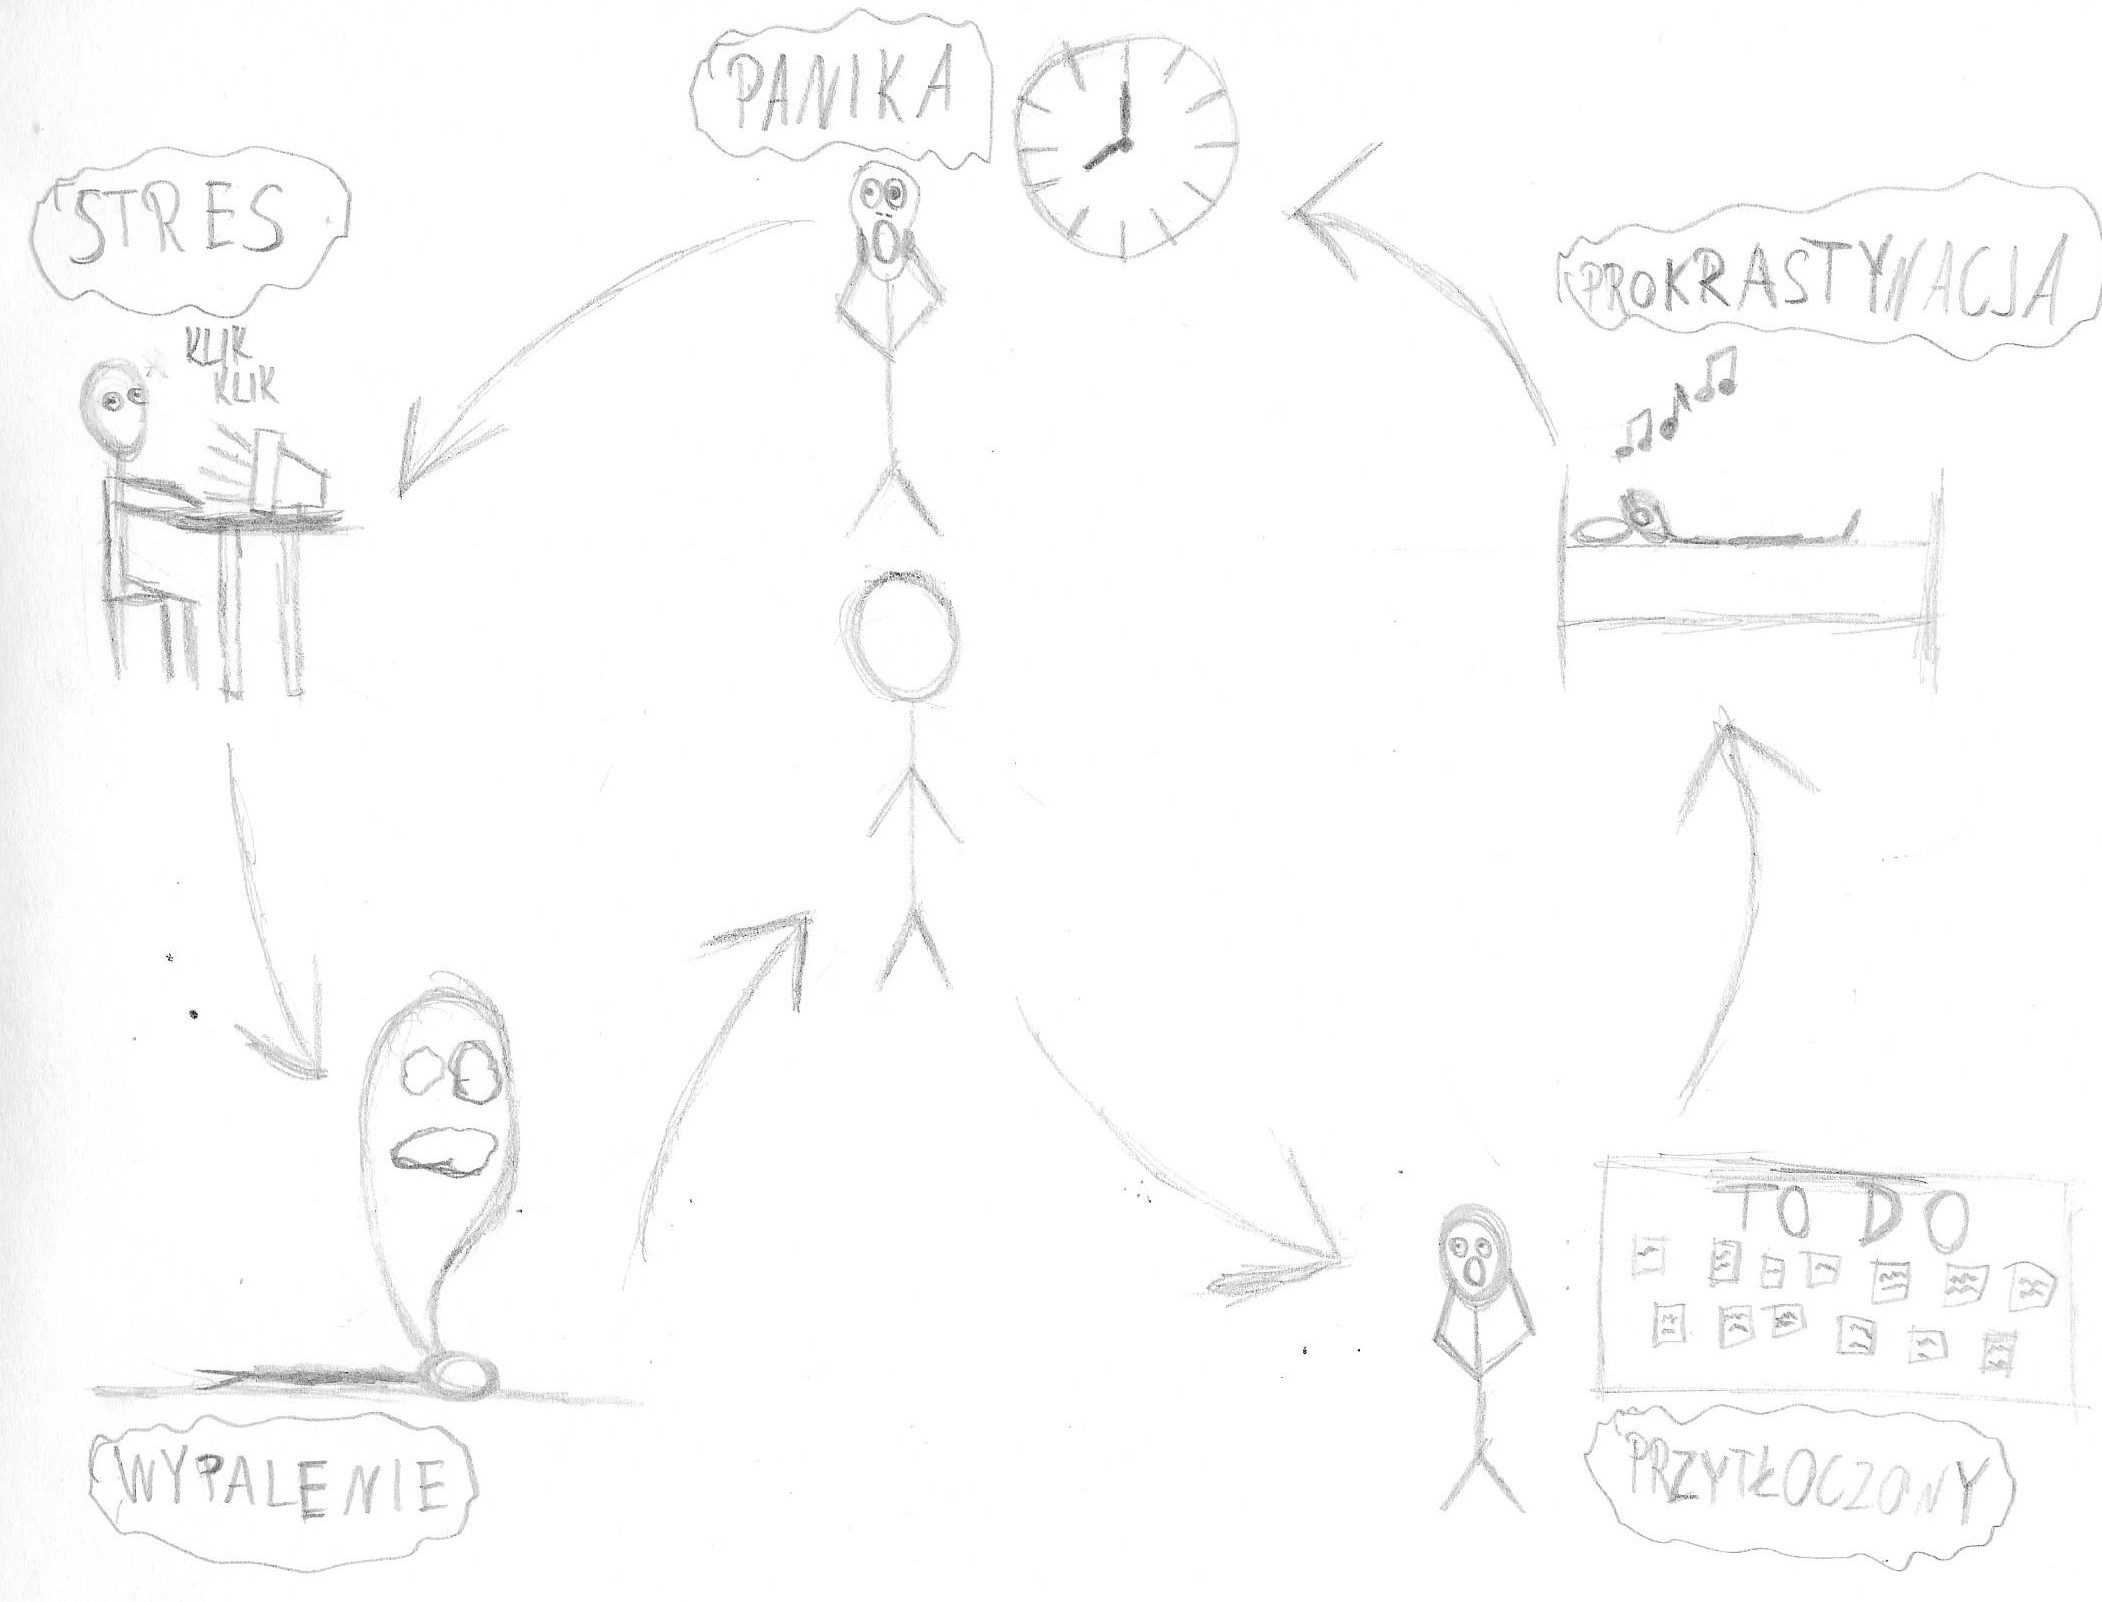
\includegraphics[width=\textwidth, height=9cm]{richpicture1}
	\caption{Użytkownik przed skorzystaniem z systemu.}
	\label{fig:rich1}
\end{figure}
\begin{figure}[h]
	\centering
	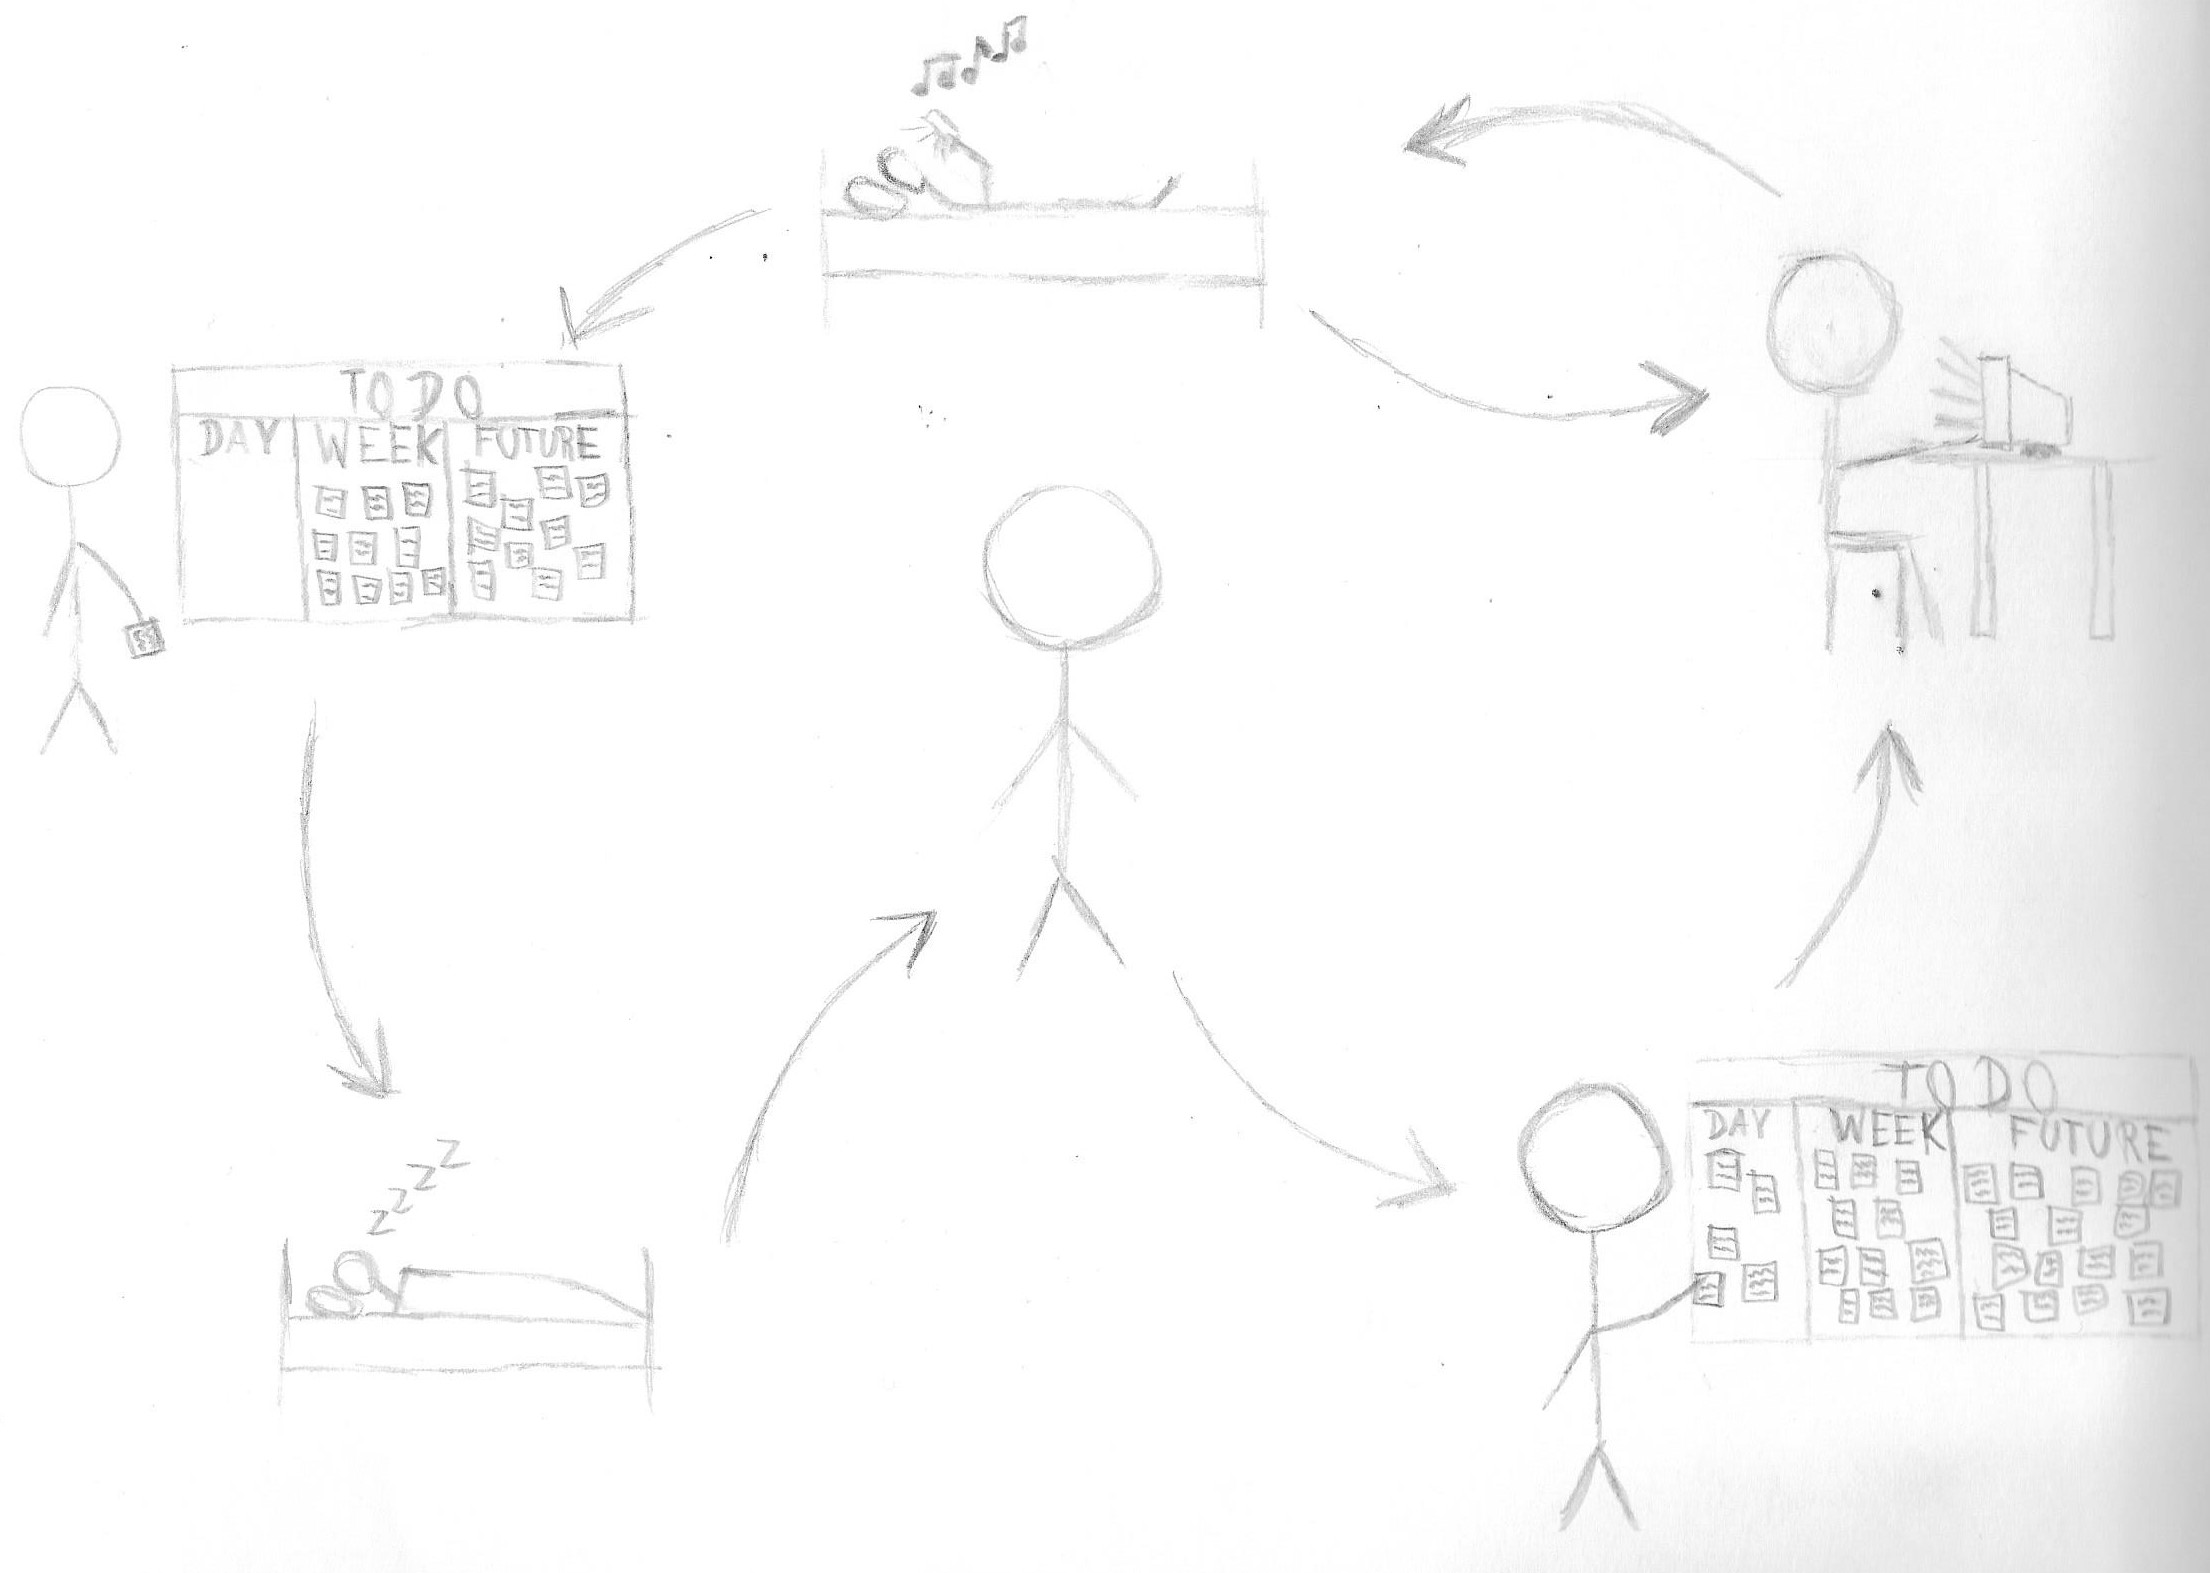
\includegraphics[width=\textwidth, height=9cm]{richpicture2}
	\caption{Użytkownik korzystający z systemu.}
	\label{fig:rich2}
\end{figure}
\section {Konkurencyjne rozwiązania}
\subsection{Brain Focus}
\subsubsection{O Aplikacji}
Brain Focus jest to aplikacja mobilna, pozwalająca na odmierzanie czasu w sesjach z przerwami.
 Nie jest skomplikowana w użyciu, poprzez dosyć prosty wygląd co nie rozprasza użytkownika.
 Daje ona możliwość pełnej modyfikacji ich minutnika od czasu pracy i długości przerwy, do ich ilości i częstości występowania dłuższej przerwy.
 Posiada ona również funkcję blokowania innych aplikacji, by pomóc użytkownikom pozostać skupionym.
 Aplikacja również daje nam dostęp do ogólnych statystyk użytkownika tj. średnia długość pracy nad zadaniami itp.
\subsubsection{Zalety i wady}
Na pewno zaletami aplikacji jest jej prosty wygląd,
 jak i pełna możliwość modyfikacji minutnika,
 który może zostać przypisany do konkretnego zadania.
\vspace{0,5cm}
 \\Do jej wad można zaliczyć brak nagradzania użytkownika za jego poświęcony czas z aplikacją.
\vspace{0,5cm}
\\Chcielibyśmy wykorzystać ich zalety w formie pełnej modyfikacji minutnika razem z możliwością przypisywania go do zadania,
 ponieważ w naszym rozwiązaniu oczekujemy,
 że użytkownicy będą mieli bardzo zróżnicowane projekty, co spowoduję potrzebę modyfikacji minutnika pod projekty.
\subsubsection{Model biznesowy i popularność}
Aplikacja ta używa modelu biznesowego `freemium` gdzie w podstawowej formie aplikacja nie wysyła powiadomień
 oraz ma limitowane tworzenie kategorii zadań natomiast w wersji Pro
 po zakupieniu mamy nielimitowane tworzenie kategorii zadań,
 dostajemy dostęp do powiadomień w aplikacji,
 uzyskujemy dostęp do jej widget'u,
 jak i dostęp do wszystkich przyszłych funkcji aplikacji.
\vspace{0,5cm}\\Obecnie popularność aplikacji na platformie Google Play w liczbie pobrań przekracza 1000000 pobrań.
\subsection{Productivity Challenge Timer}
\subsubsection{O Aplikacji}
PCT jest to aplikacja mobilna, pozwalająca na dodawanie projektów,
 nad którymi chcemy pracować i umożliwia nam pracę nad nimi z odliczaniem czasu pracy w formie minutnika.
 Wraz z systematycznym pracowaniem nad naszymi projektami,
 aplikacja nagradza nas nowymi rangami w zależności od poświęconego czasu i systematyczności.
 Aplikacja prowadzi podstawowe statystyki tj. liczba sesji wykonana przy danym projekcie w danym dniu
 czy średnia liczba sesji w tygodniu. Jest także system osiągnięć, które zdobywamy wraz z używaniem aplikacji.
\subsubsection{Zalety i wady}
Zaletą aplikacji jest to, że aplikacja wynagradza użytkownika za spędzany z nią czas w formie rang,
 które ulepszają się wraz z systematyczną pracą.
\vspace{0,5cm}
\\Do jej wad możemy zaliczyć ograniczenie możliwości tworzenia projektów do 4 w darmowej wersji aplikacji,
ograniczona edycja minutnika, jak i duże kary za brak systematyczności w formie dużych spadków w rangach użytkownika.
System może również powodować przyśpieszone wypalenie, bądź nieefektywną prace poprzez zachęcanie do ciągłej, nieprzerwanej pracy.
\vspace{0,5cm}
\\Chcielibyśmy wykorzystać formę gratyfikacji użytkownika w formie rang, tak by nasza aplikacja
 jednocześnie motywowała naszych użytkowników do dalszej pracy z systemem, jak i
 wykazywała postępy osiągane przez użytkownika.
\subsubsection{Model biznesowy i popularność}
Aplikacja używa modelu `freemium` gdzie w darmowej wersji jesteśmy ograniczeni do stworzenia 4 projektów,
 otrzymujemy agresywne reklamy w aplikacji, jak i mamy ograniczoną liczbę osiągnięć do zdobycia.
 Natomiast w wersji PRO mamy nieograniczoną liczbę projektów do tworzenia, nie dostajemy reklam,
 odblokowujemy dostęp do obecnie niemożliwych do zdobycia osiągnięć, jak i w przyszłości nowych.
\vspace{0,5cm}\\
Obecnie popularność aplikacji na platformie Google Play w liczbie pobrań przekracza 500000 pobrań.
\subsection{Habitica}
\subsubsection{O Aplikacji}
Habitica to aplikacja mobilna, jak i webowa, w której tworzymy swoją postać i ulepszamy ją poprzez wykonywanie zadań.
 Użytkownik na początku tworzy postać, którą rozwija wraz z używaniem aplikacji.
 Postać posiada statystyki tj. siła, inteligencja, kondycja i percepcja.
 Wraz z wykonywaniem zadań, postać zadaję określone punkty obrażeń stworą,
 które jeśli zostaną pokonane, dają postaci punkty doświadczenia.
 Punkty doświadczenia po osiągnięciu pewnego progu, zwiększają poziom postaci.
 Statystyki możemy zwiększać poprzez dodawanie ich za dostępne punkty po osiągnięciu poziomu bądź z posiadanych przedmiotów.
\subsubsection{Zalety i wady}
Zaletą aplikacji jest widoczna gamifikacja, co przyciąga dużą grupę użytkowników,
 która kojarzy owe systemy doświadczenia i statystyk z gier komputerowych.
 Zaletą również jest element aplikacji, gdzie tworzymy drużynę z innymi graczami, by pokonać silniejsze stwory.
\vspace{0,5cm}
\\Wadą aplikacji jest brak możliwości śledzenia czasu na wykonanie zadania bądź brak jakiegokolwiek minutnika, zachęcającego do systematycznej pracy.
 Wadą także jest duże skomplikowanie aplikacji, co może odstraszyć nowych użytkowników.
\vspace{0,5cm}\\
Chcielibyśmy wykorzystać system statystyk konta w naszym systemie,
 ponieważ idzie to w parze z osiąganiem rang jako forma nagradzania użytkownika za spędzany czas.
\subsubsection{Model biznesowy i popularność}
Model biznesowy aplikacji opiera się o mikro transakcje, gdzie możemy wykupywać walutę premium w grze,
 by osiągnąć rzeczy niedostępne dla użytkowników bez owej waluty tj. wyglądy postaci,
 misje na otrzymanie towarzyszy w formie chowańców czy możliwość zresetowania postaci.
\vspace{0,5cm}\\
Obecnie popularność aplikacji na platformie Google Play w liczbie pobrań przekracza 1000000 pobrań
 oraz szacowana ilość całkowita wszystkich użytkowników oscyluje w granicach 4000000 użytkowników.
\subsection{Pomodone}
\subsubsection{O Aplikacji}
Pomodone to aplikacja webowa, jak i mobilna, gdzie mamy możliwość dodawania zadań do wykonania
 oraz mamy możliwość włączenia sesji pracy nad konkretnym zadaniem.
 Aplikacja pozwala nam na zablokowanie konkretnych stron bądź aplikacji,
 by zapewnić użytkownikom pełne skupienie nad wykonanym zadaniem.
\subsubsection{Zalety i wady}
Zaletą aplikacji jest jej wieloplatformowość,
 ponieważ jest dostępna na każdym systemie operacyjnym, na komputerach stacjonarnych, systemach mobilnych,
 jak i przeglądarkach w formie widget'u.
 Kolejną zaletą jest też duża możliwość modyfikacji minutnika.
\vspace{0,5cm}
\\ Wadą jest pozornie prosty wygląd aplikacji, w której bardzo łatwo można się zgubić, będąc nowym użytkownikiem.
Wadą także można by nazwać brak podpowiedzi dla użytkownika, jeśli zgubiłby się w aplikacji.
\vspace{0,5cm}
\\Chcielibyśmy nie popełnić błędu, gdzie użytkownik bardzo łatwo może się zgubić w aplikacji,
 dlatego chcemy wytworzyć system, gdzie wszystkie potrzebne informacje zawsze będą na widoku
 oraz użytkownicy również będą mieli do dyspozycji podpowiedzi, jeśli mieliby trudności z korzystania z systemu.
\subsubsection{Model biznesowy i popularność}
Model biznesowy aplikacji używa płatnej subskrypcji do korzystania z aplikacji.
 Dla studentów jest rok darmowej subskrypcji dzięki programowi Github Education.
\vspace{0,5cm}\\
Obecnie popularność aplikacji na platformie Google Play w liczbie pobrań przekracza 10000 pobrań.
 Brak informacji o użytkownikach z innych platform.
\section {Propozycja rozwiązania}
Użytkownik będzie miał do wyboru kilka schematów organizacji pracy, każdy z nich będzie szanował ideę skupienia na energii zamiast na czasie.
\\Każda czynność będzie dodawała jedną, bądź kilka z 4 statystyk albo odnawiała jedną, bądź kilka z 4 energii.
\\Statystyki i odpowiadające energie:
\\Siła dla zadań fizycznych oraz odpowiadająca jej energia ciała.
\\Twórczość dla zadań artystycznych oraz odpowiadająca jej energia emocji.
\\Inteligencja dla zadań umysłowych oraz odpowiadająca jej energia umysłu.
\\Biegłość dla zadań humanistyczno-językowych oraz odpowiadające jej energia duszy.
\subsection{Projekty}
Pierwszym z nich są projekty, czyli organizacja ogólnej tematyki kierunku działań bądź konkretny plan bez wyszczególnionych celów pośrednich.
\\Użytkownik ma w tym wypadku jakiś cel, na tyle odległy, że wykonanie go nie jest możliwe podczas jednej, nieważne jak długiej, sesji pracy.
\\Przykładami mogą być tu odpowiednio nauka Python'a oraz kurs Python'a, ponieważ oba zadania wymagają czasu dużo dłuższego od maksymalnej długości ludzkiego skupienia.
\\Projekty można organizować w foldery np. w folderze programowanie backend'owe mógłbym mieć trzy projekty NodeJs, DenoJs oraz Django.
\\Projekty mogą również przybrać jedną z 2 form, statystyk bądź energii.
\\Projekty statystyk to  ćwiczenia siłowe, praca umysłowa, praca kreatywna, nauka języka itp.
\\Projekty energii to rozciąganie, medytacja, techniki oddychania itp.
\vspace{0.5cm}
\\W przypadku tego typu zadań najlepsze efekty daje systematyczna praca. Dlatego projekty polegają na:
\\Stworzeniu projektu i przypisaniu mu nazwy, folderu, statystyk bądź energii boostowanych oraz dominującej, oraz domyślnej metody pracy.
\\Na przykładzie nauki Python'a mogłoby to być:
\\nazwa: Nauka Python'a
\\folder: Programowanie
\\statystyki Wzmacniane: inteligencja
\\statystyka dominująca: inteligencja
\\domyślna metoda pracy: Pomodoro
\\Nad tak stworzonym projektem możemy teraz pracować w sesjach wybranej metodyki aż do osiągnięcia celu.
\subsection{Bullet Journal}
Drugim z nich jest Bullet Journal, czyli rozplanowywanie zadań do wykonania jako poszczególne zadania w kontekście czasu.
\\Standardowo dzieli się na zadania na dany dzień, tydzień, miesiąc, nieokreśloną przyszłość oraz po terminie, ale użytkownik może dodać dowolne przedziały czasowe.
\\Jako że ludzie często lubią oddzielać własne zadania od pracy, dodaliśmy możliwość posiadania wielu dzienników.
\subsection{Themes}
Tutaj możemy wydać zarobione podczas sesji bądź za wykonywanie zadań statystyki, aby nabyć rangi.
\\Również tutaj zakupimy nowe wyglądy oraz dźwięki dla naszej aplikacji.
\\Rangi są awatarami użytkownika, początkowo dostaje się jedną z 4 darmowych rang koale, żółwia, węża bądź leniwca.
\\Po poświęceniu pewnego czasu na prace użytkownik zapewne poczuje, że nie jest już takim leniwcem, ale jest już np. wilkiem.
\\Jest to pewna forma trofeum oraz przyswojenie sobie pewnego obrazu swojego zwierzęcia duchowego.

\section {Kontekst systemu}
Aplikacja webowa kompatybilna z większością przeglądarek i komputerów z dostępem do Internetu.
 Można z niej korzystać o dowolnej porze dnia, używając urządzeń mobilnych.
 Chcemy podzielić projekt na mikro serwisy,
 pozwoli nam to na łatwą skalowalność i późniejsze pielęgnowanie projektu.
 Nasz system będzie się składał z wielu funkcjonalności,
 z których użytkownik będzie mógł zarządzać swoją pracą tj. zarządzanie projektami,
 Bullet Journal czy Elastic Habits\cite{elastic} wspierane przez system rang,
 system energii czy system osiągnięć.
 System zarządzającymi projektami pomaga nam dzielić sobie nasze zadania na sesję o określonym wymiarze
 czasowym wybranym przez użytkownika.
 Okresy te bazowano na technikach tj. Pomodoro\cite{Pomodoro} 25/5, Ultradian Rhytmn\cite{90/30}90/30,
 flow state\cite{flow} oraz Just 5\cite{just5}.
 Wykonywanie projektów jest nagradzane statystykami, które zwiększają się w zależności, jakiego typu był projekt.
 Po spełnieniu danego warunku użytkownik może zostać nagrodzony osiągnięciem za przekroczenie pewnego kamienia milowego
 w swojej pracy nad projektem.
 Zadaniem Bullet Journal’a jest rozplanowanie pomniejszych zadań z projektu w czasie i wizualizacja ich na tablicy,
 by użytkownik mógł śledzić jakie zadania musi wykonać danego dnia, by wyrobić się w terminie.
 Elastic Habits miałby za zadanie pomóc użytkownikowi wyrobić sobie nawyk,
 poprzez poziomowanie sobie zaplanowanego zadania.
 W zależności od ogólnego samopoczucia użytkownika może on wybrać łatwiejszą bądź trudniejszą wersję zadania, dalej utrzymując nawyk wykonywania go. \\
\begin{figure}[h]
	\centering
	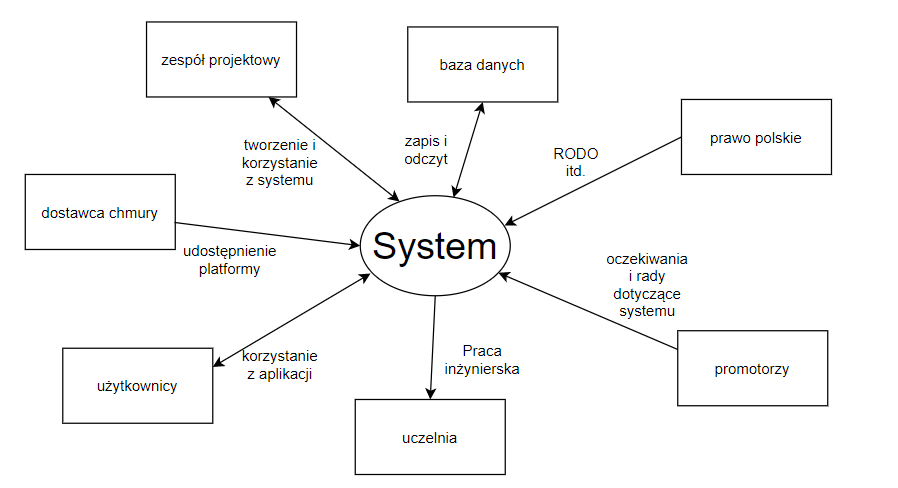
\includegraphics[width=\textwidth, height=9cm]{system}\\
	\caption{Diagram systemu}
	\label{fig:system}
\end{figure}
\section {Cele i odbiorcy systemu}
\subsection {Cele systemu}
Chcemy stworzyć nowe narzędzie do organizacji pracy z oryginalnym podejściem zaczerpniętym z systemów RPG,
 opartym na odkryciach w dziedzinie zarządzania energią\cite{Harward}.
 Chcemy, aby użytkownicy korzystający z naszego narzędzia nie zarządzali wyłącznie swoim czasem,
 ale także i energią, która jest równie ważna. Efektem będzie aplikacja internetowa.
 W przyszłości planujemy rozszerzyć system o aplikację mobilną oraz desktop'ową.
 Spodziewaną korzyścią będzie wzrost produktywności długoterminowej pośród użytkowników.
 Produktywność użytkowników moglibyśmy sprawdzać poprzez ankiety,
 porównujące czas poświęcony na zadania bez korzystania z systemu oraz z nim np. użytkownik skończył
 zaplanowane zadanie tydzień szybciej lub pracował przez 2 godziny dłużej niż bez korzystania z systemu.\\
\subsection {Udziałowcy}
\begin{tabular}{|p{3cm}|p{11cm}|}
	\hline
	\multicolumn{2}{|l|}{\textbf{Karta Udziałowca}}\\
	\hline
	Identyfikator&UOB01\\
	\hline
	Nazwa&Zespół projektowy\\
	\hline
	Opis&Zespół projektowy tworzy oraz opiekuje się systemem\\
	\hline
	Typ udziałowca&Ożywiony, bezpośredni\\
	\hline
	Punkt widzenia&Perspektywa twórców systemu\\
	\hline
	Ograniczenia&Brak\\
	\hline
	Wymagania&\\
	\hline
	\end{tabular}\\
	\begin{tabular}{|p{3cm}|p{11cm}|}
	\hline
	\multicolumn{2}{|l|}{\textbf{Karta Udziałowca}}\\
	\hline
	Identyfikator&UOB02\\
	\hline
	Nazwa&Użytkownik końcowy\\
	\hline
	Opis&Przeciętny, finalny użytkownik korzystający z aplikacji\\
	\hline
	Typ udziałowca&Ożywiony, bezpośredni\\
	\hline
	Punkt widzenia&Perspektywa użytkownika\\
	\hline
	Ograniczenia&Nie ma dostępu do warstwy technicznej — bazy danych, kodu itp.\\
	\hline
	Wymagania&\\
	\hline
	\end{tabular}\\
	\begin{tabular}{|p{3cm}|p{11cm}|}
	\hline
	\multicolumn{2}{|l|}{\textbf{Karta Udziałowca}}\\
	\hline
	Identyfikator&UOB03\\
	\hline
	Nazwa&Sponsorzy\\
	\hline
	Opis&Osoba, która finansuje projekt i egzekwuje wymagania\\
	\hline
	Typ udziałowca&Ożywiony, bezpośredni\\
	\hline
	Punkt widzenia&Perspektywa ekonomiczna\\
	\hline
	Ograniczenia&Nie powinien narzucać technologii przy tworzeniu projektu\\
	\hline
	Wymagania&\\
	\hline
	\end{tabular}\\
	\begin{tabular}{|p{3cm}|p{11cm}|}
	\hline
	\multicolumn{2}{|l|}{\textbf{Karta Udziałowca}}\\
	\hline
	Identyfikator&UOB04\\
	\hline
	Nazwa&Wydawca\\
	\hline
	Opis&Osoba, która jest odpowiedzialna za sfinalizowanie projektu i wypuszczenie go na rynek\\
	\hline
	Typ udziałowca&Ożywiony, bezpośredni\\
	\hline
	Punkt widzenia&Perspektywa ekonomiczna\\
	\hline
	Ograniczenia&Nie powinien narzucać technologii przy tworzeniu projektu\\
	\hline
	Wymagania&\\
	\hline
	\end{tabular}\\
	\begin{tabular}{|p{3cm}|p{11cm}|}
	\hline
	\multicolumn{2}{|l|}{\textbf{Karta Udziałowca}}\\
	\hline
	Identyfikator&UOB05\\
	\hline
	Nazwa&Promotorzy\\
	\hline
	Opis&Doradcy w sprawach dotyczących projektu\\
	\hline
	Typ udziałowca&Ożywiony, bezpośredni\\
	\hline
	Punkt widzenia&Perspektywa twórców projektu\\
	\hline
	Ograniczenia&Nie zawsze dostępni\\
	\hline
	Wymagania&\\
	\hline
	\end{tabular}\\
	\begin{tabular}{|p{3cm}|p{11cm}|}
	\hline
	\multicolumn{2}{|l|}{\textbf{Karta Udziałowca}}\\
	\hline
	Identyfikator&UNB01\\
	\hline
	Nazwa&Media\\
	\hline
	Opis&Strony internetowe, reklamy, artykuły, audycje itp.\\
	\hline
	Typ udziałowca&Nieożywiony, bezpośredni\\
	\hline
	Punkt widzenia&Perspektywa ekonomiczna\\
	\hline
	Ograniczenia&Zero wpływu na budowę projektu\\
	\hline
	Wymagania&\\
	\hline
	\end{tabular}\\
	\begin{tabular}{|p{3cm}|p{11cm}|}
	\hline
	\multicolumn{2}{|l|}{\textbf{Karta Udziałowca}}\\
	\hline
	Identyfikator&UNB02\\
	\hline
	Nazwa&Baza danych\\
	\hline
	Opis&Jedna, wspólna baza danych na cały system\\
	\hline
	Typ udziałowca&Nieożywiony, bezpośredni\\
	\hline
	Punkt widzenia&Perspektywa techniczna\\
	\hline
	Ograniczenia&Skończona ilość pamięci do przechowywania informacji\\
	\hline
	Wymagania&\\
	\hline
	\end{tabular}\\
	\begin{tabular}{|p{3cm}|p{11cm}|}
	\hline
	\multicolumn{2}{|l|}{\textbf{Karta Udziałowca}}\\
	\hline
	Identyfikator&UNB03\\
	\hline
	Nazwa&Prawo polskie\\
	\hline
	Opis&Zgodnie z RODO mamy obowiązek dbać o bezpieczeństwo danych osobowych wszystkich użytkowników\\
	\hline
	Typ udziałowca&Nieożywiony, bezpośredni\\
	\hline
	Punkt widzenia&Perspektywa prawna\\
	\hline
	Ograniczenia&Brak\\
	\hline
	Wymagania&\\
	\hline
	\end{tabular}\\
	\begin{tabular}{|p{3cm}|p{11cm}|}
	\hline
	\multicolumn{2}{|l|}{\textbf{Karta Udziałowca}}\\
	\hline
	Identyfikator&UNB04\\
	\hline
	Nazwa&Dostawca usług chmurowych\\
	\hline
	Opis&Serwer w chmurze odpowiedzialny za przetwarzanie wszystkich żądań pomiędzy serwisami i użytkownikami końcowymi\\
	\hline
	Typ udziałowca&Nieożywiony, bezpośredni\\
	\hline
	Punkt widzenia&Perspektywa techniczna\\
	\hline
	Ograniczenia& Sprzętowe, specyfikacja sprzętu (np. moc procesora serwerowego, przepustowość Internetu)\\
	\hline
	Wymagania&\\
	\hline
	\end{tabular}\\
\subsection {Grupa docelowa}
Z naszego rozwiązania, może skorzystać każdy.
Czy to osoba z etatem starającą się utrzymać swoją rodzinę, czy to student, który zasypany jest obowiązkami ze studiów.
Są jednak osoby, których higiena pracy wykańcza, co sprawia, że w pracy bardzo szybko tracą swoją efektywność oraz wzrasta zmęczenie.
Po pracy są oni wykończeni, nie mają czasu dla siebie ani dla rodziny.\\
Są też osoby, którym brakuje systematyczności, motywacji do pracy.\\
Do tych wszystkich osób kierujemy nasze rozwiązanie, ale chcemy, by każdy mógł znaleść w naszym systemie coś dla siebie.\\
\chapter {Analiza}
%Pozamieniać Sprint ... na odnośniki do sprintów oraz podsekcji z implementacji
\section {Wymagania}
\subsection {Wymagania ogólne i dziedzinowe}
		\begin{tabular}{|p{3cm}|p{2cm}|p{2cm}|p{6cm}|}
		\hline
		\multicolumn{4}{|p{12 cm}|}{Karta Wymagania}\\
		\hline
		Identyfikator: & W01 & Priorytet: & M — must\\
		\hline
		Nazwa & \multicolumn{3}{|p{10 cm}|}{Zwiększenie efektywności pracy użytkowników systemu}\\
		\hline
		Opis & \multicolumn{3}{|p{10 cm}|}{Końcowy produkt systemu ma za zadanie zwiększać produktywność jego użytkowników, weryfikowane jest to na podstawie prac z Harvardu i user feedbacku w postaci ankiet.}\\
		\hline
		Udziałowiec & \multicolumn{3}{|p{10 cm}|}{Wydawca, Użytkownik końcowy}\\
		\hline
		Wymagania powiązane & \multicolumn{3}{|p{10 cm}|}{Brak}\\
		\hline
		\end{tabular}\\
	\subsection {Wymagania funkcjonalne}
		\begin{tabular}{|p{3cm}|p{2cm}|p{2cm}|p{6cm}|}
		\hline
		\multicolumn{4}{|p{12 cm}|}{Karta Wymagania}\\
		\hline
		Identyfikator: & F01 & Priorytet: & M — must\\
		\hline
		Nazwa & \multicolumn{3}{|p{10 cm}|}{System Autoryzacji użytkownika}\\
		\hline
		Opis & \multicolumn{3}{|p{10 cm}|}{Jako użytkownik muszę mieć możliwość zarejestrowania się w serwisie i późniejszego logowania się}\\
		\hline
		Kryteria akceptacji & \multicolumn{3}{|p{10 cm}|}{Bezpieczny system autoryzacji zabezpieczony przed atakami na bazę danych, potwierdzenie maila po rejestracji,  jedno konta na 1 mail}\\
		\hline
		Dane wejściowe & \multicolumn{3}{|p{10 cm}|}{e-mail użytkownika, hasło użytkownika, nick}\\
		\hline
		Warunki początkowe & \multicolumn{3}{|p{10 cm}|}{Użytkownik nie posiada konta}\\
		\hline
		Warunki końcowe & \multicolumn{3}{|p{10 cm}|}{Użytkownik zarejestrował się i może się zalogować}\\
		\hline
		Sytuacje wyjątkowe & \multicolumn{3}{|p{10 cm}|}{Błędny e-mail, błędne hasło, użytkownik już posiada konto}\\
		\hline
		Szczegóły implementacji & \multicolumn{3}{|p{10 cm}|}{Historia Sprintów \ref{sec:system_autoryzacji_uzytkownika}}\\
		\hline
		Udziałowiec & \multicolumn{3}{|p{10 cm}|}{Użytkownik końcowy, Zespół projektowy}\\
		\hline
		Wymagania powiązane & \multicolumn{3}{|p{10 cm}|}{Brak}\\
		\hline
		\end{tabular}\\
		\newline
		\vspace*{0,2 cm}
		\newline
		\begin{tabular}{|p{3cm}|p{2cm}|p{2cm}|p{6cm}|}
		\hline
		\multicolumn{4}{|p{12 cm}|}{Karta Wymagania}\\
		\hline
		Identyfikator: & F02 & Priorytet: & M — must (musi być)\\
		\hline
		Nazwa & \multicolumn{3}{|p{10 cm}|}{System statystyk}\\
		\hline
		Opis & \multicolumn{3}{|p{10 cm}|}{Jako użytkownik podczas postępowania w używaniu aplikacji chciałbym widzieć swój postęp w pracy nad projektami w postaci statystyk}\\
		\hline
		Kryteria akceptacji & \multicolumn{3}{|p{10 cm}|}{Obliczanie statystyk użytkownika na podstawie wykonywanych projektów.}\\
		\hline
		Dane wejściowe & \multicolumn{3}{|p{10 cm}|}{czas poświęcony na zadanie, statystyki ulepszane przez zadanie, główna statystyka ulepszana przez zadanie}\\
		\hline
		Warunki początkowe & \multicolumn{3}{|p{10 cm}|}{Użytkownik jest zalogowany, zakończył sesję pracy}\\
		\hline
		Warunki końcowe & \multicolumn{3}{|p{10 cm}|}{Aktualizacja statystyk}\\
		\hline
		Sytuacje wyjątkowe & \multicolumn{3}{|p{10 cm}|}{Użytkownik nie wykonał żadnej sesji}\\
		\hline
		Szczegóły implementacji & \multicolumn{3}{|p{10 cm}|}{Historia Sprintów \ref{sec:system_statystyk}}\\
		\hline
		Udziałowiec & \multicolumn{3}{|p{10 cm}|}{Użytkownik końcowy, Zespół projektowy}\\
		\hline
		Wymagania powiązane & \multicolumn{3}{|p{10 cm}|}{F03, F05}\\
		\hline
		\end{tabular}\\
		\newline
		\vspace*{0,2 cm}
		\newline
		\begin{tabular}{|p{3cm}|p{2cm}|p{2cm}|p{6cm}|}
		\hline
		\multicolumn{4}{|p{12 cm}|}{Karta Wymagania}\\
		\hline
		Identyfikator: & F03 & Priorytet: & M — must (musi być)\\
		\hline
		Nazwa & \multicolumn{3}{|p{10 cm}|}{System zarządzania energią użytkownika}\\
		\hline
		Opis & \multicolumn{3}{|p{10 cm}|}{Jako użytkownik chcę, żeby aplikacja śledziła moje zasoby energetyczne, by widzieć swój stan energii.}\\
		\hline
		Kryteria akceptacji & \multicolumn{3}{|p{10 cm}|}{Zmiana zasobów energii użytkownika przy wykonywaniu konkretnych projektów lub przerw.}\\
		\hline
		Dane wejściowe & \multicolumn{3}{|p{10 cm}|}{Czas poświęcony na zadanie, statystyki ulepszane przez zadanie, główna statystyka ulepszana przez zadanie}\\
		\hline
		Warunki początkowe & \multicolumn{3}{|p{10 cm}|}{Użytkownik jest zalogowany, została wykonana sesja pracy.}\\
		\hline
		Warunki końcowe & \multicolumn{3}{|p{10 cm}|}{Zmniejszenie/zwiększenie statusu energii}\\
		\hline
		Sytuacje wyjątkowe & \multicolumn{3}{|p{10 cm}|}{Brak energii, nie wykonano żadnej sesji}\\
		\hline
		Szczegóły implementacji & \multicolumn{3}{|p{10 cm}|}{Historia Sprintów \ref{sec:system_zarzadzania_energia_uzytkownika}}\\
		\hline
		Udziałowiec & \multicolumn{3}{|p{10 cm}|}{Użytkownik końcowy, Zespół projektowy}\\
		\hline
		Wymagania powiązane & \multicolumn{3}{|p{10 cm}|}{F02, F05}\\
		\hline
		\end{tabular}\\
		\newline
		\vspace*{0,2 cm}
		\newline
		\begin{tabular}{|p{3cm}|p{2cm}|p{2cm}|p{6cm}|}
		\hline
		\multicolumn{4}{|p{12 cm}|}{Karta Wymagania}\\
		\hline
		Identyfikator: & F04 & Priorytet: & M — must (musi być)\\
		\hline
		Nazwa & \multicolumn{3}{|p{10 cm}|}{System zarządzania folderami użytkowników}\\
		\hline
		Opis & \multicolumn{3}{|p{10 cm}|}{Jako użytkownik chciałbym mieć możliwość dodawania, usuwania i edycji folderów dla projektów.}\\
		\hline
		Kryteria akceptacji & \multicolumn{3}{|p{10 cm}|}{Użytkownik ma możliwość dodawania, usuwania i edycji folderów.}\\
		\hline
		Dane wejściowe & \multicolumn{3}{|p{10 cm}|}{Ikona, nazwa folderu}\\
		\hline
		Warunki początkowe & \multicolumn{3}{|p{10 cm}|}{Użytkownik jest zalogowany.}\\
		\hline
		Warunki końcowe & \multicolumn{3}{|p{10 cm}|}{Stworzenie folderu, usunięcie folderu, edycja folderu}\\
		\hline
		Sytuacje wyjątkowe & \multicolumn{3}{|p{10 cm}|}{Nie podano danych}\\
		\hline
		Szczegóły implementacji & \multicolumn{3}{|p{10 cm}|}{Historia Sprintów \ref{sec:system_zarzadzania_energia_uzytkownika}}\\
		\hline
		Udziałowiec & \multicolumn{3}{|p{10 cm}|}{Użytkownik końcowy, Zespół projektowy}\\
		\hline
		Wymagania powiązane & \multicolumn{3}{|p{10 cm}|}{F05}\\
		\hline
		\end{tabular}\\
		\newline
		\vspace*{0,2 cm}
		\newline
		\begin{tabular}{|p{3cm}|p{2cm}|p{2cm}|p{6cm}|}
		\hline
		\multicolumn{4}{|p{12 cm}|}{Karta Wymagania}\\
		\hline
		Identyfikator: & F05 & Priorytet: & M — must (musi być)\\
		\hline
		Nazwa & \multicolumn{3}{|p{10 cm}|}{System zarządzania projektami użytkowników}\\
		\hline
		Opis & \multicolumn{3}{|p{10 cm}|}{Jako użytkownik chciałbym mieć możliwość dodawania, usuwania i śledzenia moich projektów}\\
		\hline
		Kryteria akceptacji & \multicolumn{3}{|p{10 cm}|}{Użytkownik ma możliwość dodawania, usuwania i śledzenia projektów.}\\
		\hline
		Dane wejściowe & \multicolumn{3}{|p{10 cm}|}{Nazwa projektu, statystyki ulepszane, dominująca statystyka, folder, metoda pracy}\\
		\hline
		Warunki początkowe & \multicolumn{3}{|p{10 cm}|}{Użytkownik jest zalogowany.}\\
		\hline
		Warunki końcowe & \multicolumn{3}{|p{10 cm}|}{Stworzenie projektu, usunięcie projektu, edycja projektu}\\
		\hline
		Sytuacje wyjątkowe & \multicolumn{3}{|p{10 cm}|}{Nie podano danych}\\
		\hline
		Szczegóły implementacji & \multicolumn{3}{|p{10 cm}|}{Historia Sprintów \ref{sec:system_zarzadzania_projektami_uzytkownikow}}\\
		\hline
		Udziałowiec & \multicolumn{3}{|p{10 cm}|}{Użytkownik końcowy, Zespół projektowy}\\
		\hline
		Wymagania powiązane & \multicolumn{3}{|p{10 cm}|}{F02,F04}\\
		\hline
		\end{tabular}\\
		\newline
		\vspace*{0,2 cm}
		\newline
		\begin{tabular}{|p{3cm}|p{2cm}|p{2cm}|p{6cm}|}
		\hline
		\multicolumn{4}{|p{12 cm}|}{Karta Wymagania}\\
		\hline
		Identyfikator: & F06 & Priorytet: & M — must (musi być)\\
		\hline
		Nazwa & \multicolumn{3}{|p{10 cm}|}{System zarządzania dziennikami}\\
		\hline
		Opis & \multicolumn{3}{|p{10 cm}|}{Jako użytkownik chcę mieć możliwość zarządzania dziennikami do planowania zadań.}\\
		\hline
		Kryteria akceptacji & \multicolumn{3}{|p{10 cm}|}{Użytkownik może dodawać, usuwać, edytować swoje dzienniki.}\\
		\hline
		Dane wejściowe & \multicolumn{3}{|p{10 cm}|}{Nazwa, ikona, połączony projekt}\\
		\hline
		Warunki początkowe & \multicolumn{3}{|p{10 cm}|}{Użytkownik jest zalogowany}\\
		\hline
		Warunki końcowe & \multicolumn{3}{|p{10 cm}|}{Dodano, usunięto, edytowano dziennik}\\
		\hline
		Sytuacje wyjątkowe & \multicolumn{3}{|p{10 cm}|}{Nie podano danych}\\
		\hline
		Szczegóły implementacji & \multicolumn{3}{|p{10 cm}|}{Historia Sprintów \ref{sec:system_zarzadzania_dziennikami}}\\
		\hline
		Udziałowiec & \multicolumn{3}{|p{10 cm}|}{Użytkownik końcowy, Zespół projektowy}\\
		\hline
		Wymagania powiązane & \multicolumn{3}{|p{10 cm}|}{Brak}\\
		\hline
		\end{tabular}\\
		\newline
		\vspace*{0,2 cm}
		\newline
		\begin{tabular}{|p{3cm}|p{2cm}|p{2cm}|p{6cm}|}
		\hline
		\multicolumn{4}{|p{12 cm}|}{Karta Wymagania}\\
		\hline
		Identyfikator: & F07 & Priorytet: & M — must (musi być)\\
		\hline
		Nazwa & \multicolumn{3}{|p{10 cm}|}{System zarządzania stronami dziennika}\\
		\hline
		Opis & \multicolumn{3}{|p{10 cm}|}{Jako użytkownik chcę mieć możliwość zarządzania stronami dziennika.}\\
		\hline
		Kryteria akceptacji & \multicolumn{3}{|p{10 cm}|}{Użytkownik może dodawać, usuwać, edytować swoje strony w dziennikach.}\\
		\hline
		Dane wejściowe & \multicolumn{3}{|p{10 cm}|}{Nazwa, ikona, dziennik, początek zakresu dni wyświetlany przez stronę w formie liczby, koniec zakresu}\\
		\hline
		Warunki początkowe & \multicolumn{3}{|p{10 cm}|}{Użytkownik jest zalogowany, użytkownik ma utworzony dziennik}\\
		\hline
		Warunki końcowe & \multicolumn{3}{|p{10 cm}|}{Dodano, usunięto, edytowano dziennik}\\
		\hline
		Sytuacje wyjątkowe & \multicolumn{3}{|p{10 cm}|}{Nie podano danych, podano niepoprawny zakres}\\
		\hline
		Szczegóły implementacji & \multicolumn{3}{|p{10 cm}|}{Historia Sprintów \ref{sec:system_zarzadzania_stronami_dziennika}}\\
		\hline
		Udziałowiec & \multicolumn{3}{|p{10 cm}|}{Użytkownik końcowy, Zespół projektowy}\\
		\hline
		Wymagania powiązane & \multicolumn{3}{|p{10 cm}|}{Brak}\\
		\hline
		\end{tabular}\\
		\newline
		\vspace*{0,2 cm}
		\newline
		\begin{tabular}{|p{3cm}|p{2cm}|p{2cm}|p{6cm}|}
		\hline
		\multicolumn{4}{|p{12 cm}|}{Karta Wymagania}\\
		\hline
		Identyfikator: & F08 & Priorytet: & M — must (musi być)\\
		\hline
		Nazwa & \multicolumn{3}{|p{10 cm}|}{System zarządzania zadaniami w dziennikach}\\
		\hline
		Opis & \multicolumn{3}{|p{10 cm}|}{Jako użytkownik chcę mieć możliwość zarządzania zadaniami w dziennikach.}\\
		\hline
		Kryteria akceptacji & \multicolumn{3}{|p{10 cm}|}{Użytkownik może dodawać, usuwać, edytować swoje zadania w dziennikach.}\\
		\hline
		Dane wejściowe & \multicolumn{3}{|p{10 cm}|}{Nazwa, opis, powiązany projekt, termin wykonania, tagi}\\
		\hline
		Warunki początkowe & \multicolumn{3}{|p{10 cm}|}{Użytkownik jest zalogowany, użytkownik ma utworzony dziennik z przynajmniej jedną stroną}\\
		\hline
		Warunki końcowe & \multicolumn{3}{|p{10 cm}|}{Dodano, usunięto, edytowano dziennik}\\
		\hline
		Sytuacje wyjątkowe & \multicolumn{3}{|p{10 cm}|}{Nie podano danych}\\
		\hline
		Szczegóły implementacji & \multicolumn{3}{|p{10 cm}|}{Historia Sprintów \ref{sec:system_zarzadzania_zadaniami_w_dziennikach}}\\
		\hline
		Udziałowiec & \multicolumn{3}{|p{10 cm}|}{Użytkownik końcowy, Zespół projektowy}\\
		\hline
		Wymagania powiązane & \multicolumn{3}{|p{10 cm}|}{Brak}\\
		\hline
		\end{tabular}\\
		\newline
		\vspace*{0,2 cm}
		\newline
		\begin{tabular}{|p{3cm}|p{2cm}|p{2cm}|p{6cm}|}
		\hline
		\multicolumn{4}{|p{12 cm}|}{Karta Wymagania}\\
		\hline
		Identyfikator: & F09 & Priorytet: & M — must (musi być)\\
		\hline
		Nazwa & \multicolumn{3}{|p{10 cm}|}{Zarządzanie czasomierzem}\\
		\hline
		Opis & \multicolumn{3}{|p{10 cm}|}{Jako użytkownik chcę mieć możliwość zarządzania czasomierzami.}\\
		\hline
		Kryteria akceptacji & \multicolumn{3}{|p{10 cm}|}{Użytkownik może dodawać, usuwać, edytować swoje czasomierze.}\\
		\hline
		Dane wejściowe & \multicolumn{3}{|p{10 cm}|}{Nazwa, skrót, czas sesji pracy, czas krótkiej przerwy, czas długiej przerwy, czas nadpracy, interwał przerw krótkich i długich}\\
		\hline
		Warunki początkowe & \multicolumn{3}{|p{10 cm}|}{Użytkownik jest zalogowany}\\
		\hline
		Warunki końcowe & \multicolumn{3}{|p{10 cm}|}{Dodano, usunięto, edytowano czasomierz}\\
		\hline
		Sytuacje wyjątkowe & \multicolumn{3}{|p{10 cm}|}{Nie podano danych}\\
		\hline
		Szczegóły implementacji & \multicolumn{3}{|p{10 cm}|}{Historia Sprintów \ref{sec:zarzadzanie_czasomierzem}}\\
		\hline
		Udziałowiec & \multicolumn{3}{|p{10 cm}|}{Użytkownik końcowy, Zespół projektowy}\\
		\hline
		Wymagania powiązane & \multicolumn{3}{|p{10 cm}|}{Brak}\\
		\hline
		\end{tabular}\\
		\newline
		\vspace*{0,2 cm}
		\newline
		\begin{tabular}{|p{3cm}|p{2cm}|p{2cm}|p{6cm}|}
		\hline
		\multicolumn{4}{|p{12 cm}|}{Karta Wymagania}\\
		\hline
		Identyfikator: & F10 & Priorytet: & M — must (musi być)\\
		\hline
		Nazwa & \multicolumn{3}{|p{10 cm}|}{system sesji pracy}\\
		\hline
		Opis & \multicolumn{3}{|p{10 cm}|}{Jako użytkownik chcę mieć możliwość uruchomiania czasomierza, by rozpocząć sesję pracy bądź przerwę.}\\
		\hline
		Kryteria akceptacji & \multicolumn{3}{|p{10 cm}|}{Użytkownik może uruchamiać, jak i zatrzymywać czasomierz sesji pracy oraz przerw.}\\
		\hline
		Dane wejściowe & \multicolumn{3}{|p{10 cm}|}{Wybrany projekt, wybrane zadanie, domyślny czasomierz}\\
		\hline
		Warunki początkowe & \multicolumn{3}{|p{10 cm}|}{Użytkownik jest zalogowany, został wybrany projekt bądź zadanie.}\\
		\hline
		Warunki końcowe & \multicolumn{3}{|p{10 cm}|}{Uruchomienie, jak i zatrzymanie sesji pracy bądź przerwy}\\
		\hline
		Sytuacje wyjątkowe & \multicolumn{3}{|p{10 cm}|}{Nie wybrano projektu, nie wybrano zadania}\\
		\hline
		Szczegóły implementacji & \multicolumn{3}{|p{10 cm}|}{Historia Sprintów \ref{sec:system_sesji_pracy}}\\
		\hline
		Udziałowiec & \multicolumn{3}{|p{10 cm}|}{Użytkownik końcowy, Zespół projektowy}\\
		\hline
		Wymagania powiązane & \multicolumn{3}{|p{10 cm}|}{Brak}\\
		\hline
		\end{tabular}\\
		\newline
		\vspace*{0,2 cm}
		\newline
		\begin{tabular}{|p{3cm}|p{2cm}|p{2cm}|p{6cm}|}
		\hline
		\multicolumn{4}{|p{12 cm}|}{Karta Wymagania}\\
		\hline
		Identyfikator: & F11 & Priorytet: & W – won't \\
		\hline
		Nazwa & \multicolumn{3}{|p{10 cm}|}{System osiągnięć użytkownika}\\
		\hline
		Opis & \multicolumn{3}{|p{10 cm}|}{Jako użytkownik chciałbym co jakiś czas być nagradzany za osiągnięcia przy dochodzeniu do kamieni milowych podczas korzystania z aplikacji}\\
		\hline
		Kryteria akceptacji & \multicolumn{3}{|p{10 cm}|}{Użytkownik otrzymuje osiągnięcia za przekroczenie pewnych kamieni milowych}\\
		\hline
		Udziałowiec & \multicolumn{3}{|p{10 cm}|}{Użytkownik końcowy, Zespół projektowy}\\
		\hline
		Wymagania powiązane & \multicolumn{3}{|p{10 cm}|}{Brak}\\
		\hline
		\end{tabular}\\
		\newline
		\vspace*{0,2 cm}
		\newline
		\begin{tabular}{|p{3cm}|p{2cm}|p{2cm}|p{6cm}|}
		\hline
		\multicolumn{4}{|p{12 cm}|}{Karta Wymagania}\\
		\hline
		Identyfikator: & F12 & Priorytet: & W – won't\\
		\hline
		Nazwa & \multicolumn{3}{|p{10 cm}|}{System rankingowy użytkowników}\\
		\hline
		Opis & \multicolumn{3}{|p{10 cm}|}{Jako użytkownik chciałbym mieć dostęp do tablic rankingowych, gdzie mógłbym porównywać swoje osiągnięcia z innymi użytkownikami.}\\
		\hline
		Kryteria akceptacji & \multicolumn{3}{|p{10 cm}|}{Użytkownik jest w stanie sprawdzić swoją pozycję w rankingu dotyczącą danego projektu}\\
		\hline
		Udziałowiec & \multicolumn{3}{|p{10 cm}|}{Użytkownik końcowy, Zespół projektowy}\\
		\hline
		Wymagania powiązane & \multicolumn{3}{|p{10 cm}|}{Brak}\\
		\hline
		\end{tabular}\\
		\newline
		\vspace*{0,2 cm}
		\newline
		\begin{tabular}{|p{3cm}|p{2cm}|p{2cm}|p{6cm}|}
		\hline
		\multicolumn{4}{|p{12 cm}|}{Karta Wymagania}\\
		\hline
		Identyfikator: & F13 & Priorytet: & W – won't \\
		\hline
		Nazwa & \multicolumn{3}{|p{10 cm}|}{System znajomych użytkowników}\\
		\hline
		Opis & \multicolumn{3}{|p{10 cm}|}{Jako użytkownik chciałbym móc dodawać innych użytkowników do swojej listy znajomych, żeby sprawdzać ich postępy}\\
		\hline
		Kryteria akceptacji & \multicolumn{3}{|p{10 cm}|}{Użytkownik może dodawaj znajomych, wyświetlanych w formie listy, u których może sprawdzać ich postępy}\\
		\hline
		Udziałowiec & \multicolumn{3}{|p{10 cm}|}{Użytkownik końcowy, Zespół projektowy}\\
		\hline
		Wymagania powiązane & \multicolumn{3}{|p{10 cm}|}{Brak}\\
		\hline
		\end{tabular}\\
		\newline
		\vspace*{0,2 cm}
		\newline
		\begin{tabular}{|p{3cm}|p{2cm}|p{2cm}|p{6cm}|}
		\hline
		\multicolumn{4}{|p{12 cm}|}{Karta Wymagania}\\
		\hline
		Identyfikator: & F14 & Priorytet: & W – won't\\
		\hline
		Nazwa & \multicolumn{3}{|p{10 cm}|}{Energy Assistant}\\
		\hline
		Opis & \multicolumn{3}{|p{10 cm}|}{Jako użytkownik chciałbym, żeby moje rzeczywiste poziomy energii były lepiej rozpoznawane.}\\
		\hline
		Kryteria akceptacji & \multicolumn{3}{|p{10 cm}|}{Użytkownik zależnie jaki prowadzi tryb życia bądź w zależności od jego warunków fizycznych, jak i psychicznych miałby dostosowywaną ilość energii na dany dzień}\\
		\hline
		Udziałowiec & \multicolumn{3}{|p{10 cm}|}{Użytkownik końcowy, Zespół projektowy}\\
		\hline
		Wymagania powiązane & \multicolumn{3}{|p{10 cm}|}{Brak}\\
		\hline
		\end{tabular}\\
		\newline
		\vspace*{0,2 cm}
		\newline
		\begin{tabular}{|p{3cm}|p{2cm}|p{2cm}|p{6cm}|}
		\hline
		\multicolumn{4}{|p{12 cm}|}{Karta Wymagania}\\
		\hline
		Identyfikator: & F15 & Priorytet: & W – won't\\
		\hline
		Nazwa & \multicolumn{3}{|p{10 cm}|}{Elastic Habits}\\
		\hline
		Opis & \multicolumn{3}{|p{10 cm}|}{Jako użytkownik chciałbym móc podzielić swoje zadanie na różne poziomy trudności.}\\
		\hline
		Kryteria akceptacji & \multicolumn{3}{|p{10 cm}|}{Użytkownik może wybrać z dany poziom trudności zadania, by wyrobić sobie nawyk wykonywania go.}\\
		\hline
		Udziałowiec & \multicolumn{3}{|p{10 cm}|}{Użytkownik końcowy, Zespół projektowy}\\
		\hline
		Wymagania powiązane & \multicolumn{3}{|p{10 cm}|}{Brak}\\
		\hline
		\end{tabular}\\
	\subsection {Wymagania poza funkcjonalne}
	\begin{tabular}{|p{3cm}|p{2cm}|p{2cm}|p{6cm}|}
		\hline
		\multicolumn{4}{|p{12 cm}|}{Karta Wymagania}\\
		\hline
		Identyfikator: & NF01 & Priorytet: & M – must (musi być)\\
		\hline
		Nazwa & \multicolumn{3}{|p{10 cm}|}{C\#}\\
		\hline
		Opis & \multicolumn{3}{|p{10 cm}|}{Backend powinien być napisany w C\#}\\
		\hline
		Udziałowiec & \multicolumn{3}{|p{10 cm}|}{Zespół projektowy, Wydawca}\\
		\hline
		Wymagania powiązane & \multicolumn{3}{|p{10 cm}|}{Brak}\\
		\hline
		\end{tabular}\\
		\newline
		\vspace*{0,2 cm}
		\newline
		\begin{tabular}{|p{3cm}|p{2cm}|p{2cm}|p{6cm}|}
		\hline
		\multicolumn{4}{|p{12 cm}|}{Karta Wymagania}\\
		\hline
		Identyfikator: & NF02 & Priorytet: & M – must (musi być)\\
		\hline
		Nazwa & \multicolumn{3}{|p{10 cm}|}{React}\\
		\hline
		Opis & \multicolumn{3}{|p{10 cm}|}{Frontend powinien być napisany, korzystając z biblioteki React.}\\
		\hline
		Udziałowiec & \multicolumn{3}{|p{10 cm}|}{Zespół projektowy, Wydawca}\\
		\hline
		Wymagania powiązane & \multicolumn{3}{|p{10 cm}|}{Brak}\\
		\hline
		\end{tabular}\\
		\newline
		\vspace*{0,2 cm}
		\newline
		\begin{tabular}{|p{3cm}|p{2cm}|p{2cm}|p{6cm}|}
		\hline
		\multicolumn{4}{|p{12 cm}|}{Karta Wymagania}\\
		\hline
		Identyfikator: & NF03 & Priorytet: & M – must (musi być)\\
		\hline
		Nazwa & \multicolumn{3}{|p{10 cm}|}{Czas wdrożenia}\\
		\hline
		Opis & \multicolumn{3}{|p{10 cm}|}{System należy wdrożyć do końca semestru zimowego 2020/2021}\\
		\hline
		Udziałowiec & \multicolumn{3}{|p{10 cm}|}{Zespół projektowy, Promotorzy, Uczelnia, Wydawca}\\
		\hline
		Wymagania powiązane & \multicolumn{3}{|p{10 cm}|}{Brak}\\
		\hline
		\end{tabular}\\
		\newline
		\vspace*{0,2 cm}
		\newline
		\begin{tabular}{|p{3cm}|p{2cm}|p{2cm}|p{6cm}|}
		\hline
		\multicolumn{4}{|p{12 cm}|}{Karta Wymagania}\\
		\hline
		Identyfikator: & NF04 & Priorytet: & M – must (musi być)\\
		\hline
		Nazwa & \multicolumn{3}{|p{10 cm}|}{System powinien być dostępny 24 godziny na dobę, 7 dni w tygodniu}\\
		\hline
		Opis & \multicolumn{3}{|p{10 cm}|}{Dostęp do systemu powinien być umożliwiony w dowolnej chwili danego dnia}\\
		\hline
		Udziałowiec & \multicolumn{3}{|p{10 cm}|}{Zespół projektowy, Użytkownik końcowy, Wydawca}\\
		\hline
		Wymagania powiązane & \multicolumn{3}{|p{10 cm}|}{Brak}\\
		\hline
		\end{tabular}\\
	\subsection {Wymagania na środowisko docelowe}
	\begin{tabular}{|p{3cm}|p{2cm}|p{2cm}|p{6cm}|}
		\hline
		\multicolumn{4}{|p{12 cm}|}{Karta Wymagania}\\
		\hline
		Identyfikator: & ŚD01 & Priorytet: & M – must (musi być)\\
		\hline
		Nazwa & \multicolumn{3}{|p{10 cm}|}{Kompatybilność z komputerami}\\
		\hline
		Opis & \multicolumn{3}{|p{10 cm}|}{Produkt końcowy musi być przystosowany do korzystania w przeglądarce na komputerach.}\\
		\hline
		Kryteria akceptacji & \multicolumn{3}{|p{10 cm}|}{System responsywny testowany na przeglądarkach Google Chrome i Mozilla Firefox}\\
		\hline
		Udziałowiec & \multicolumn{3}{|p{10 cm}|}{Zespół projektowy, Użytkownik końcowy, Wydawca}\\
		\hline
		Wymagania powiązane & \multicolumn{3}{|p{10 cm}|}{Brak}\\
		\hline
		\end{tabular}\\
	\section {Wymagania jakościowe i inne}
	\begin{itemize}
		\item System szyfrowania danych użytkowników: szyfrowanie haseł użytkowników
		\item Responsywny system przystosowany dla przeglądarek Google Chrome i Mozilla Firefox
		\item System dostępny 24 godziny na dobę z wyłączeniem prac technicznych
		\item System ma być łatwy w obsłudze – średnio 5 kliknięć na wykonanie dowolnej akcji.
	\end{itemize}
\section{Przypadki użycia oraz diagramy (w trakcie przerabiania i tworzenia nowych)}
\begin{figure}[h]
	\centering
	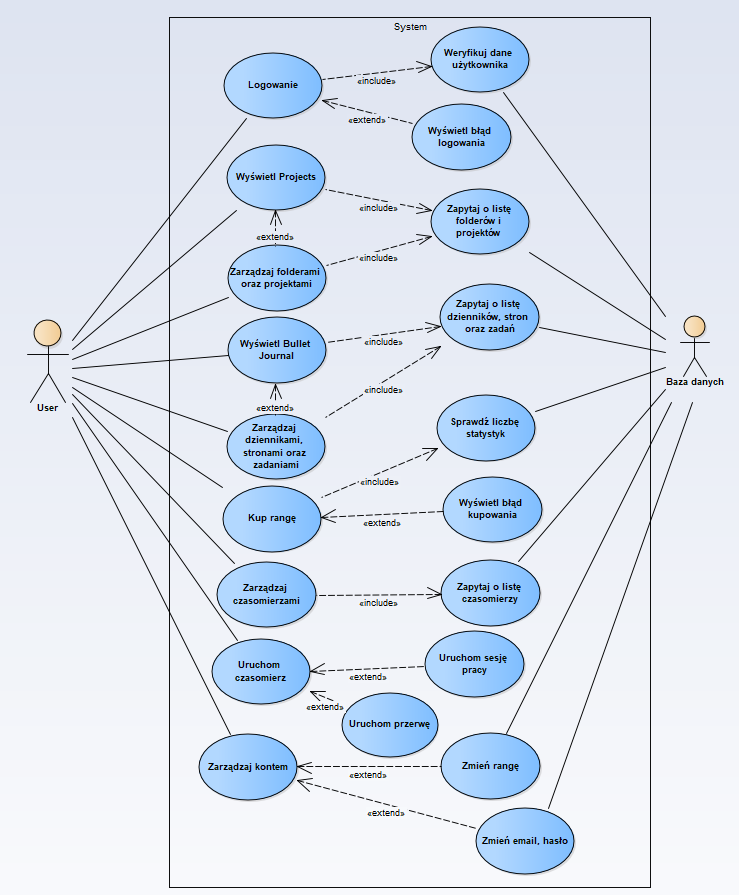
\includegraphics[width=\textwidth, height=14cm]{systemusecase}\\
	\caption{Use case dla całego systemu}
	\label{fig:usecase}
\end{figure}
\begin{figure}[h]
	\centering
	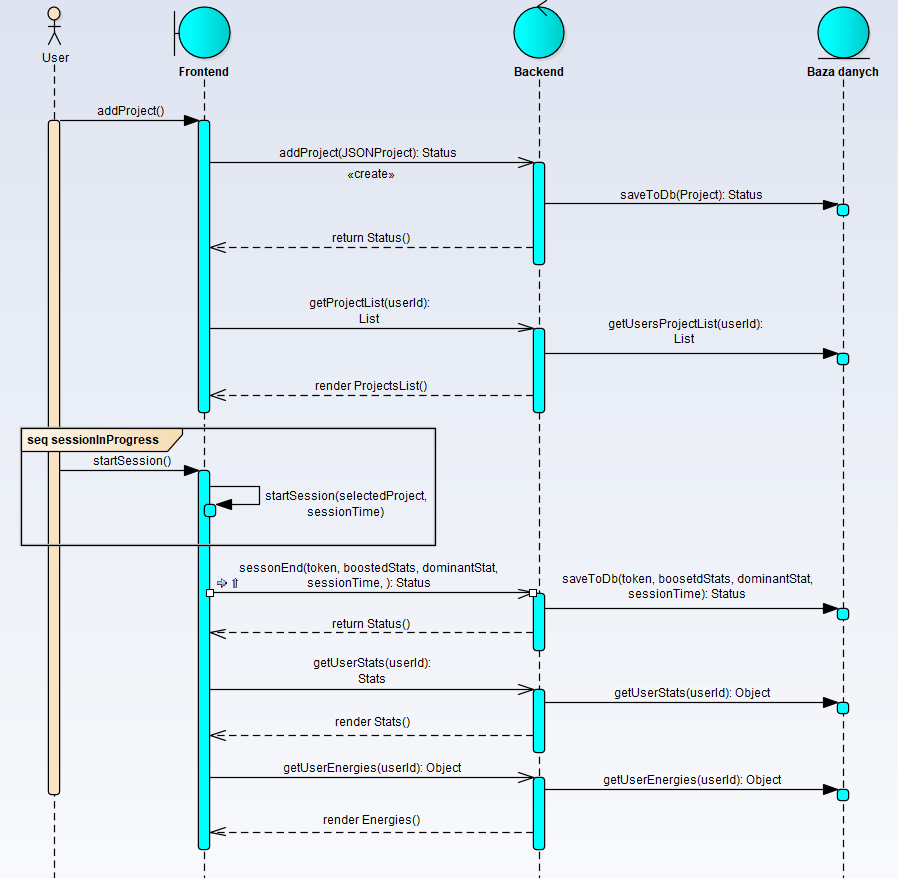
\includegraphics[width=\textwidth, height=9cm]{sekwencji}\\
	\caption{Diagram sekwencji dla dodawania projektu oraz włączania sesji}
	\label{fig:seq1}
\end{figure}
\begin{figure}[h]
	\centering
	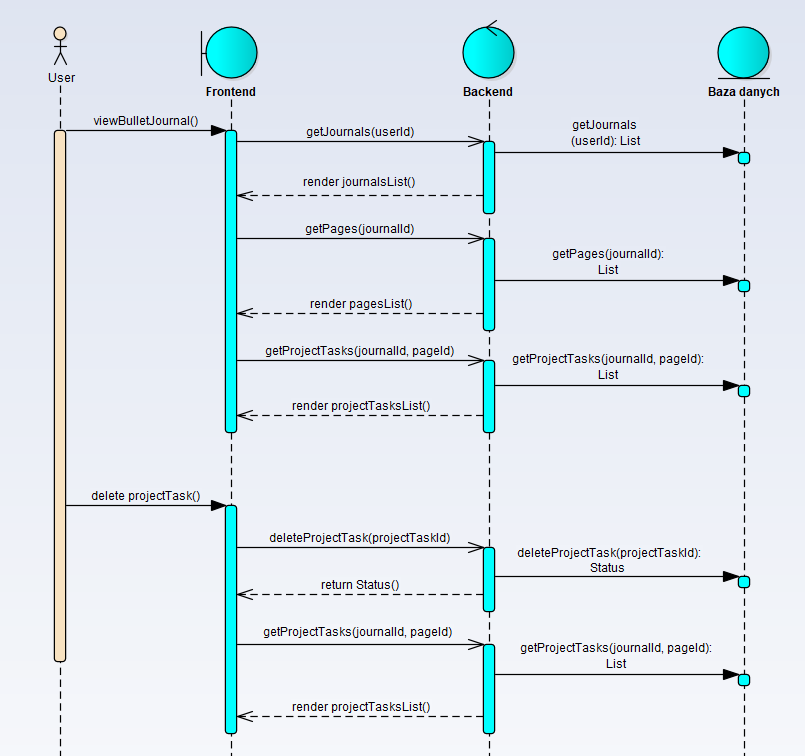
\includegraphics[width=\textwidth, height=9cm]{sekwencji1}\\
	\caption{Diagram sekwencji dla załadowania strony Bullet Journal’a oraz usuwania zadania}
	\label{fig:seq2}
\end{figure}
\chapter {Planowanie}
\section{Metodyka pracy}
Tradycyjne podejście do tworzenia oprogramowania nie było możliwe do zastosowania z uwagi na nasze płynne, dośc ogólne plany.
 Dlatego zadecydowaliśmy, że dobrym dla nas rozwiązaniem jest Scrumban, który łączy podążanie sprintami z metodologii Scrum
 oraz posiadanie tablicy zadań z metodologii Kanban\cite{agile}.
 Sprinty wymuszają na nas ciągłą, stałą pracę, by co tydzień wypuszczać nowe wersje naszego systemu.
 Zapewnia to stałą motywację do pracy, by nie osiągnąć punktu długotrwałej stagnacji w projekcie.
 Tablica zadań z metodologii Kanban pozwala nam na jasne podzielenie zadań w zespole projektowym
 oraz ułatwia określenie, w jakim stopniu dane zadanie jest wykonane.
 Wybraliśmy tę metodykę ze względu na fakt, że nasz system jest dość nowatorski w swojej kategorii,
 przez co wymaga stałej weryfikacji przez użytkowników.
 
 
\section{Narzędzia}
\subsection {Komunikacja}
Do komunikacji w zespole użyliśmy darmowej wersji Slack`a. Jedyną wadą był brak rozmów wideo.\\
Aby zapełnić tę lukę, stworzyliśmy sobie darmowy pokój na stronie Whereby, gdzie w zespole nieprzekraczającym 4
osób mogliśmy się swobodnie porozumiewać.\\
Wybór padł na Slack`a ze względu na możliwość zintegrowania go z narzędziami do CI/CD oraz repozytoriów.\\
Pozwala to na posiadanie informacji o wszystkich aktualnych działaniach całego zespołu w jednym miejscu.\\
Tablice z zadaniami posiadamy na platformie Azure DevOps, która również pozwala na tworzenie sprintów.\\
\subsection{Repozytorium oraz CI \textbackslash CD}
Repozytorium naszego projektu powstało na Github'ie. Zintegrowaliśmy go z platformą Azure DevOps, 
która pozwala nam na zbudowanie każdego komponentu projektu od razu po aktualizacji naszego kodu w repozytorium.\\
Jeżeli projekt udało się zbudować na głównej gałęzi, nasze świeżo zbudowane kontenery wysyłane są do chmury.\\
\subsection{Cloud}
W chmurze postawiliśmy na konteneryzacje naszych projektów, która pozwala na łatwe
skalowanie oraz pozostanie niezależnym od maszyny hostującej. Google Cloud został wybrany na dostawce rozwiązań chmurowych.\\
Postanowiliśmy wykorzystać technologie Kubernetes do skalowania oraz zarządzania naszymi kontenerami. Pozwala ona pozostać w miarę możliwości
niezależnym od dostawcy chmurowego (decyzja ta też została podjęta ze względu na wcześniejszą architekturę mikro serwisową).
\section{Technologie}
Sczegółowo omówione w \ref{subsec:bib_front} oraz \ref{subsec:bib_back}.
		\begin{itemize}
			\item React — wybrany ze wględu na popularność, chęć zdobycia kompetencji w zawodowo opłacalnej technologii.
			\item Redux — użyty z uwagi na liczne komponenty wymieniające miedzy sobą informacje.
			\item MUI — wykorzystany z uwagi na dobrze działające oraz wyglądające komponenty. 
			\item TypeScript — dodany w projekcie później, aby rozwiązać problemy utrzymania integracji na linii frontend-backend.
			\item C\# — wybrany z uwagi na doświadczenie z technologią.
			\item .NET Core — brak poważnych alternatyw dla framework'ów dla C\#.
			\item MongoDB — wybrany ponad inne rozwiązania NoSQL'owe z uwagi na łatwość integracji w C\#.
			\item Docker/Kubernetes — wybrany z uwagi na uniezalżnienie od środowiska produkcyjnego.
		\end{itemize}

\chapter {Projektowanie}

\section {Architektura projektu}
Aplikacja webowa Gamitude została wykonana w architekturze wielowarstwowej typu klient-serwer.
Interfejs użytkownika został wykonany w technologi SPA (single page application).
Naturalnym więc było podzielenie całej aplikacji na 2 repozytoria Frontend'u i Backend'u.
Komunikacja pomiędzy nimi opiera się na protokole HTTP/HTTPS.\\
\begin{figure}[H]
	\centering
	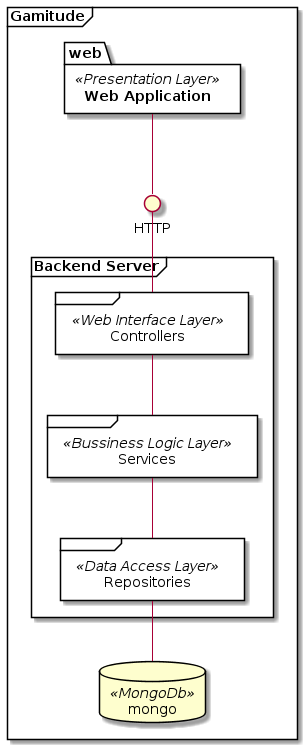
\includegraphics[scale=0.5]{gamitude_overview}\\
	\caption{Uproszczona architektura}
	\label{fig:overwiewarch}
\end{figure}


\subsection{Frontend}
Aplikacja web'owa została podzielona na komponenty z zachowaniem większości zasad atomic designu.\\
Atomic design\cite{atomicdesign} to strategia tworzenia komponentów w sposób zapewniający jak największe użycie wtórne kodu.\\
Zamiast tradycyjnego podejścia podziału na komponenty i strony, mamy tutaj rozbicie na atomy, molekuły, organizmy, szablony oraz strony.\\
Atomy to najmniejsze komponenty, otrzymują one swój stan z zewnątrz.\\
Molekuły grupują atomy i przekazują im stan.\\
Organizmy grupują atomy z molekułami oraz pilnują interakcji między nimi.\\
Szablony odpowiadają za rozmieszczenie elementów na stronie.\\
Strony wyświetlają pozostałe elementy oraz odpowiadają na nawigacje.\\
W naszym projekcie nie stosujemy szablonów z uwagi na wykorzystanie elementów Grid z Material-UI a stany i interakcje przenieśliśmy do Redux'a.\\
\subsection{Backend}
Aplikacja serwerowa została podzielona na warstwy, przedstawione na obrazku \ref{fig:overwiewarch}.
W warstwie dostępu do bazy danych został wykorzystany wzorzec projektowy repozytorium lub repozytorium serwis.
Pozwala on na zamknięcie logiki potrzebnej do pozyskania danych z bazy danych.
Dzięki temu nasza logika biznesowa jest oddzielona od infrastruktury.
Każdy obiekt w bazie danych posiada swoje repozytorium.
Każdy serwis może korzystać z wielu repozytoriów, co pozwala na tworzenie bardziej złożonych struktur.
Wykorzystany został także wzorzec projektowy wstrzykiwania zależności.
Dzięki temu w każdym miejscu projektu możemy łatwo uzyskać dostęp do potrzebnych nam elementów np. Konfiguracji.
Także pozwala nam on na łatwą podmianę danego komponentu aplikacji poprzez zarejestrowanie innej implementacji danego interfejsu.\\
\subsection{Baza Danych}
Ze względu na zwinne podejście zespołu do wytwarzania oprogramowania, głównym czynnikiem, którym zespół kierował się przy wyborze bazy danych, jest jej łatwa skalowalność.
System w trakcie prac ewoluował, przez co dodatkowym czynnikiem przy wybieraniu bazy jest jej łatwa edycja, by dostosować ją do potrzeb wymagań. 
Wybraliśmy bazę danych MongoDB, która jest bazą NoSQL do naszego projektu, przez wzgląd na oba powyższe czynniki. Bonusem przy wyborze MongoDB są niskie koszty finansowe oraz łatwiejsza skalowalność kosztem braku transakcji.
\subsection{Chmura}
Wdrożyliśmy nasza aplikacje do chmury za pośrednictwem aplikacji Kubernetes, pozwoliło to nam pozostać w miarę możliwości
niezależnym od dostawcy chmurowego. Dziś korzystamy z chmury Google'a.
Wdrożyliśmy technikę CI/CD, która pozwala na zbudowanie oraz aktualizacje rozwiązania przy każdej aktualizacji głównej gałęzi naszych repozytoriów.
\begin{figure}[h]
	\centering
	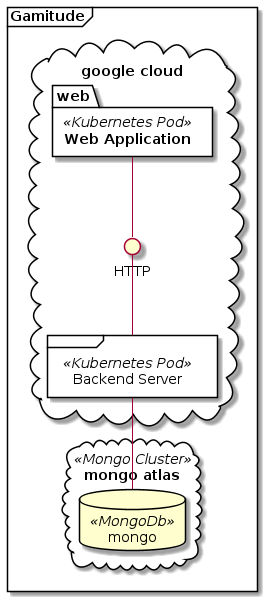
\includegraphics[scale=0.5]{gamitude_cloud_overview}\\
	\caption{Architektura chmury}
	\label{fig:db}
\end{figure}
\chapter {Implementacja rozwiązania}
\section{Frontend}
\subsection{Wykorzystane biblioteki}
\label{subsec:bib_front}
\subsubsection{Material-UI}
\label{subsec:mui}
Material-UI\cite{material-ui} składa się z 3 części:
\begin{itemize}
	\item Core — komponenty z dostosowywalną funkcjonalnością oraz wyglądem,
		duże możliwości dostosowywania za pomocą make styles opisanych w podrozdziale nr \ref{subsec:style}.
	\item Icons — biblioteka ikonek.
	\item Lab — eksperymentalne komponenty.
\end{itemize}
Zmodyfikowane wersje komponentów z Core'a tworzą praktycznie całą naszą aplikację.

\subsubsection{React}
\label{subsec:react}
React\cite{react} to deklaratywna biblioteka dla języka JavaScript ułatwiająca tworzenie interaktywnych UI.\\
 Wykorzystuje stany, aby ułatwiać renderowanie oraz re-renderowanie odpowiednych komponentów.\\
 Sam React tylko opisuje co zrobić, faktycznym renderowanie elementów zajmuje się biblioteka react-dom\cite{react-dom}.\\
 React-dom'a można używać jako pure albo z JSX-em.\\
 W wersji pure tworzymy elementy za pomocą React.createElement(nazwaTagu, tekst, dzieci) co jest dość niewygodne.\\
 Aby poprawić intuicyjnośc kodu oraz ułatwić pisanie elementów strony stworzono JSX-a.\\
 JSX to specjalny język imitujący HTML-a, który jest tłumaczony przez Babel'a do wersji pure.\\
 \begin{figure}[H]
	\centering
	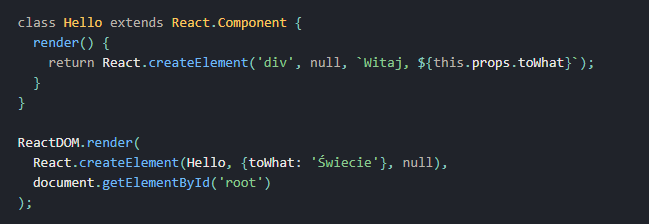
\includegraphics[scale=0.5]{implementacja/frontend/react_no_jsx}\\
	\caption{Przykład kodu w Reactie bez użycia JSX-a}
	\label{fig:react_no_jsx}
\end{figure}
 \begin{figure}[H]
	\centering
	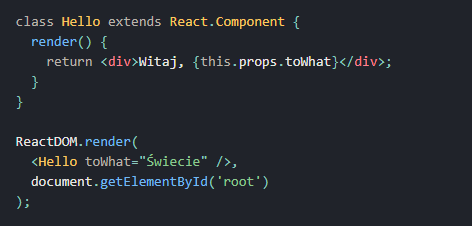
\includegraphics[scale=0.5]{implementacja/frontend/react_jsx}\\
	\caption{Ten sam kod z użyciem jsx'a}
	\label{fig:react_jsx}
\end{figure}
Babel nie jest obecny w naszych dependencjach, ponieważ używamy biblioteki Typescript\cite{typescript}, który i tak jest wewnętrznie kompilowany przez Babel'a.\\
 Do uruchamiania aplikacji Reactowej używamy react-scripts\cite{react-scripts}, które przepuszczają aplikacje przez WebPack'a.\\
 Cały ten skomplikowany setup jest automatycznie konfigurowany przy tworzeniu projektu za pomocą create-react-app.\\
\subsubsection{Redux}
\label{subsec:redux}
Redux\cite{redux} jest przewidywalnym, opiniowanym kontenerem globalnego stanu dla aplikacji JavaScript'owych\\
Konkretna implementacja dla React'a znajduje się w bibliotece react-redux\cite{react-redux},
 a sam redux definiuje tylko, podobnie jak React, strukture.
W skład tej struktury wchodzą:
\begin{itemize}
	\item Store — niemodyfikowalny objekt javascript'owy zawierający cały stan aplikacji.
	\item Root reducer — funkcja przyjmująca reducery i zwracająca nowy obiekt store'a.
	\item Reducer — fukcja przyjmująca stan obecny oraz akcje i zwracająca nowy stan obiektu.
	\item Akcja — fukcje dispatch'ujące akcje do reducer'ów, jako jedyne mogą zmieniać stan store'a.
\end{itemize}
Dodatkowo występuje też pojęcie selectora, czyli zmemoizowanej funkcji zwracającej część store'a w celu uniknięcia zbędnych re-renderów.\\
Do tworzenia tych funkcji używamy biblioteki reselect\cite{reselect}.\\
W projekcie wykorzystujemy Redux'a do łatwego współdzielenia stanu między komponentami oraz stronami naszej aplikacji.\\
Jest to dla nas świetne rozwiązanie ze względu na wykorzystanie czasomierza na różnych stronach w różnych kontekstach.\\
W projekcie odwzorowaliśmy naszą strukture folderów dla trzymania stanu pod Redux'a.
\begin{figure}[H]
	\centering
	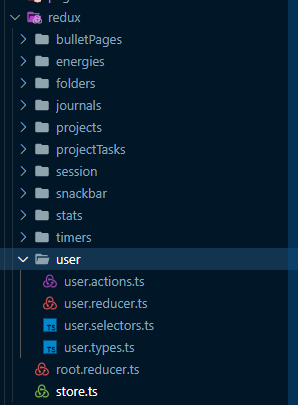
\includegraphics[scale=0.5]{implementacja/frontend/struktura_redux}\\
	\caption{Struktura folderów dla trzymania stanu naszej aplikacji w Redux'ie}
	\label{fig:struktura_redux}
\end{figure}
Dla monitorowania zmian tego globalnego stanu wykorzystujemy redux-logger'a\cite{redux-logger}.
\begin{figure}[H]
	\centering
	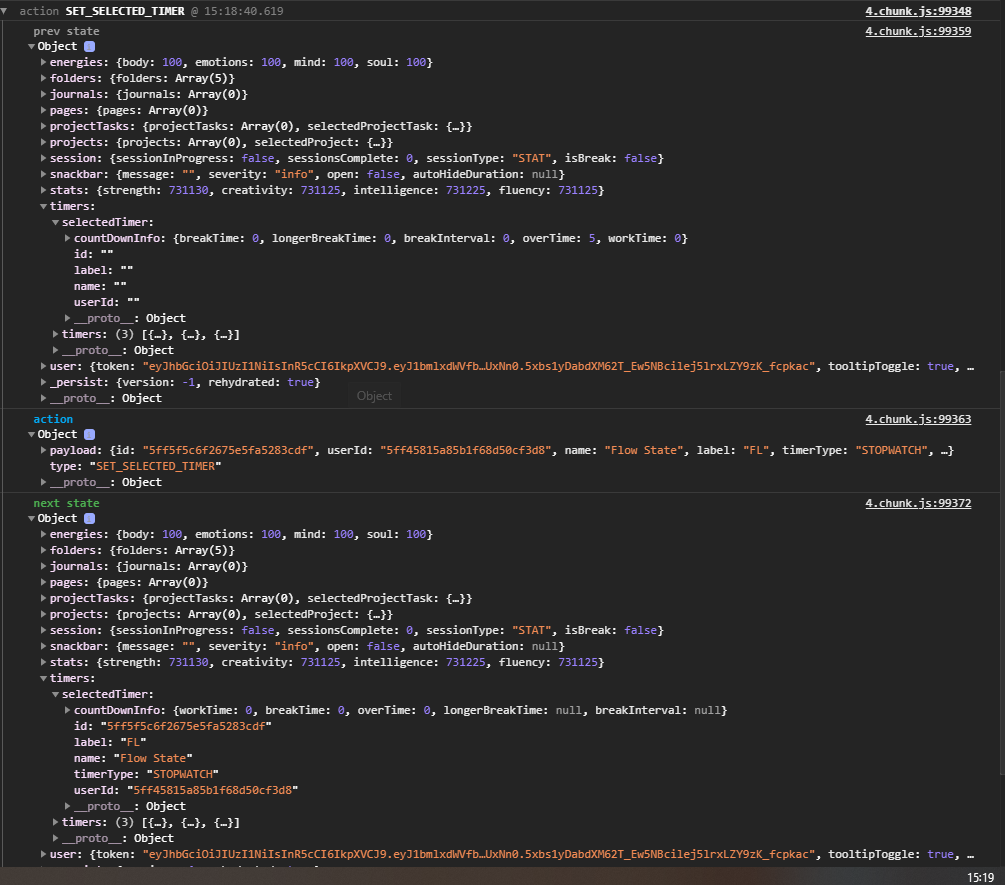
\includegraphics[scale=0.55]{implementacja/frontend/redux_logger}\\
	\caption{Przykład działania redux-logger'a w konsoli przeglądarki Brave}
	\label{fig:redux_logger}
\end{figure}
Żeby nasz store'a aktualizował się w odpowiedzi na asynchroniczne akcje z api, używamy redux-thunk'a\cite{redux-thunk}.
W celu zminimalizowania liczby żadań do API zachowujemy store'a w pamięci podręcznej przeglądarki z pomocą redux-persist\cite{redux-persist}.

\subsubsection{Axios}
Axios'a\cite{axios} używamy do wykonywania zapytań do naszego API.
 Jest to po prostu wygodniejsza i czytelniejsza metoda od korzystania z Fetch API czy XMLHttpRequest.
\subsubsection{Clsx}
Clsx'a\cite{clsx} używamy do warunkowego dodawania CSS'owych klas do komponentów.

\subsubsection{React-helmet}
React-helmet\cite{react-helmet} to prosty komponent aktualizujący element title naszej strony.
 Używamy go do wyświetlania postępu / postałego czasu sesji oraz zmian tytułu po przejściu na inną podstronę.
 Niestety przez niedawne aktualizaje Google Chrome'a wyświetlanie postępu hamuje przy przejściu na inną kartę.

\subsubsection{React-page-scroller}
React-page-scroller\cite{react-page-scroller} to prosty komponent react'owy,
 pozwalający na scrollowanie na stronach zawierających pełno-ekranowe elementy po jednej stronie.
 Wykorzystujemy go na stronie głownej naszej aplikacji.\\

\subsubsection{React-router-dom}
React-router-dom\cite{react-router-dom} to paczka imitująca routing znany z klasycznych stron renderowanych po stronie serwera.\\
W SPA tak naprawdę podmieniamy cały czas zawartość tego samego pustego na początku div'a,
 przez co tracimy możliwość korzystania z elementów przeglądarki takich jak guzik powrotu.
React-roter-dom przywraca te możliwości sprawiająć, że interakcja SPA nie różni się od interakcji z tradycyjnymi stronami.

\subsubsection{React-use}
React-use\cite{react-use} jest to biblioteka react'owych hooków.
 Są one gotowymi hookami dzielącymi się na: Sensors, UI, Side-effects,
 Animations, Lifecycles, Miscellaneous i State. 
 W projekcie głównie została wykorzystana do obsługi funkcji asynchronicznych wowoływanach za pomocą hooków stanu. \\  

\subsubsection{Use-sound}
Use-sound\cite{use-sound} to biblioteka zawierająca react'owego hooka,
 dodająca możliwość odtwarzania dzwięków na stronach razem z React-dom.
 Wykorzystujemy ja do odtwarzania dzwięków, będącymi powiadomieniami zbliżającego się końca sesji.\\ 

\subsubsection{Formik}
Formik\cite{formik} jest biblioteką do łatwego tworzenia formualarzy w Reactie.\\
 Normalnie trzebabyło tworzyć hooka — specjalną zmienną dla lokalnego stanu komponentów oraz handler akcji dla każdego pola formularza.\\
 Bardzo redukuje to przejżystość kodu, utrudnia utrzymanie, jak i samo pisanie w takim stylu zajmuje dużo czasu.\\
 Aby uniknąć tych problemów, stosujemy Formika spinającego stan formularza i monitorujego go za pomocą jednego przekazywanego obiektu.

\subsubsection{Yup}
Yup\cite{yup} jest biblioteką do walidowania formularzy za pomocą zdefiniowanych przez nas obiektów oraz zasad.

\subsubsection{Eslint}
Eslint\cite{eslint} to linter sprawdzający składnię napisanego kodu w razie wystąpienia błędów.\\  

\subsubsection{Prettier}
Prettier\cite{prettier} jest formaterem, który otrzymuje zasady, jak ma formatować kod.
 Można go rozszerzyć pluginami np. o sortowanie importów.
 Używamy go dla stosowania dobrych praktyk programowania w naszym projekcie oraz do sortowania importów w komponentach.\\

\subsubsection{Typescript}
\label{subsec:typescript}
Typescript\cite{typescript} rozszerza JavaScripta o dodawanie typów do języka. 
Przyspiesza on pracę nad kodem przez wychwytywanie problemów z typami oraz proponuje ich naprawę, zanim uruchomi się kod.
Dzieki dodaniu typów, o wiele łatwiej jest wychwytywać niespójności dotyczących danych przesyłanych w aplikacji.\\

\subsubsection{Testing-library}
Testing-library\cite{testing-library} jest to zbiór narzędzi do testowania oprogramowania.\\

\subsection{Struktura folderów}
\begin{figure}[H]
	\centering
	\includegraphics[scale=0.5]{implementacja/frontend/struktura_folderów}\\
	\caption{Struktura folderów na Frontendzie}
	\label{fig:struktura_folderów_front}
\end{figure}

\subsection{Formularze}
\label{subsec:forms}
Wszystkie formularze w naszej aplikacji są tworzone za pomocą Formika z wyglądem pól formularzy z Material-UI'a oraz walidacją z Yup'a.\\
W aplikacji stworzyliśmy specjalnie komponenty formik-form oraz formik-field, aby tworzenie formularzy było możliwe poprzez proste podanie:
\begin{itemize}
	\item Validation Schema pokazane na obrazku \ref{fig:validation_schema} — schemat walidacji pól formularza w formie obiektu.
	\item Initial Values pokazane na obrazku \ref{fig:initial_values} — wartości początkowe pól.
	\item Fields pokazane na obrazku \ref{fig:fields} — informacje o polu takie jak jego etykieta, nazwa czy typ.
\end{itemize}
\begin{figure}[H]
	\centering
	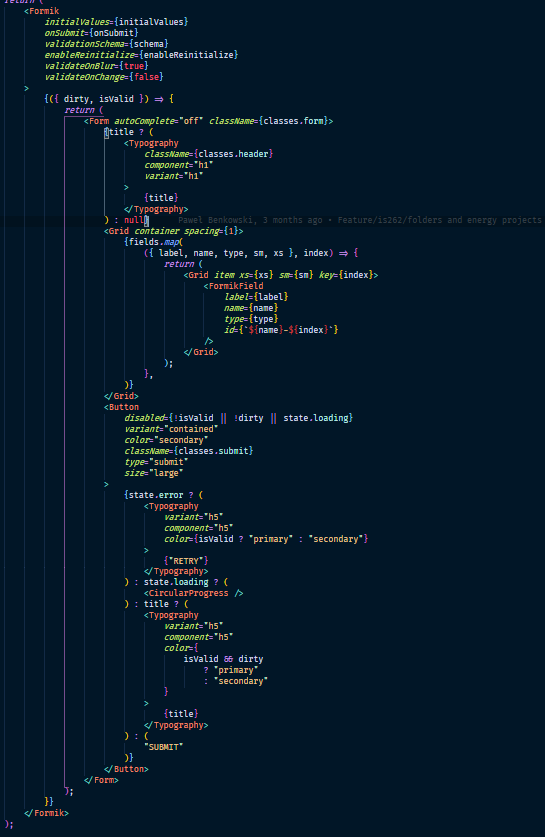
\includegraphics[scale=0.5]{implementacja/frontend/formik_form}\\
	\caption{Formik form}
	\label{fig:formik_form}
\end{figure}
\begin{figure}[H]
	\centering
	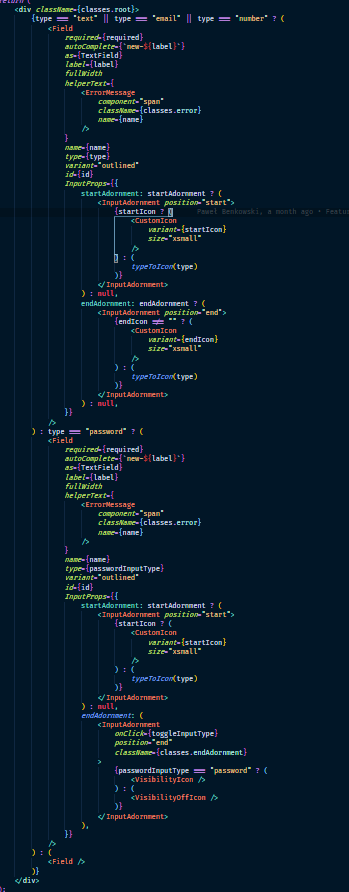
\includegraphics[scale=0.5]{implementacja/frontend/formik_field}\\
	\caption{Formik field}
	\label{fig:formik_field}
\end{figure}
\begin{figure}[H]
	\centering
	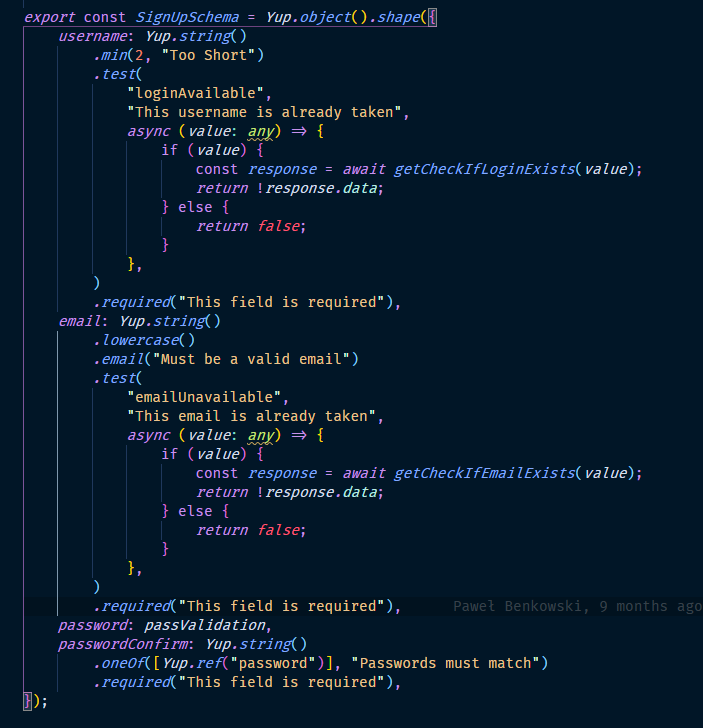
\includegraphics[scale=0.5]{implementacja/frontend/validation_schema}\\
	\caption{Przykład validation schema}
	\label{fig:validation_schema}
\end{figure}
\begin{figure}[H]
	\centering
	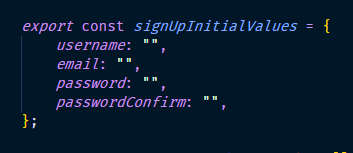
\includegraphics[scale=0.5]{implementacja/frontend/initial_values}\\
	\caption{Przykład initial values}
	\label{fig:initial_values}
\end{figure}
\begin{figure}[H]
	\centering
	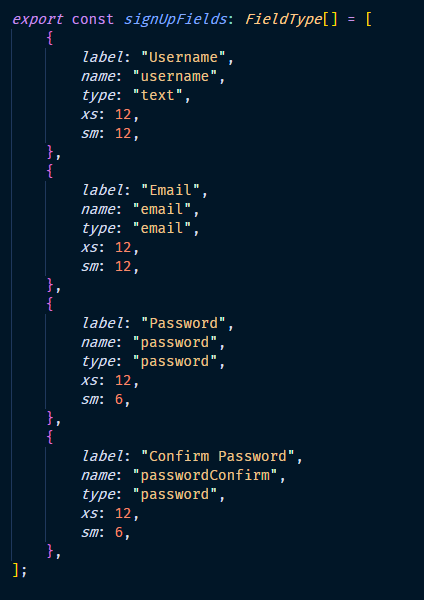
\includegraphics[scale=0.5]{implementacja/frontend/fields}\\
	\caption{Przykład fields}
	\label{fig:fields}
\end{figure}

\subsection{Tabs z Tabpanel'ami}
\label{subsec:tabs}
W aplikacji wielokrotnie korzystamy z połączenia komponentów Tabs i TabPanel — zakładek i ich zawartości.\\
Po kliknięciu danej zakładki przełączamy się na nią i wyświetlamy jej zawartość.
\begin{figure}[H]
	\centering
	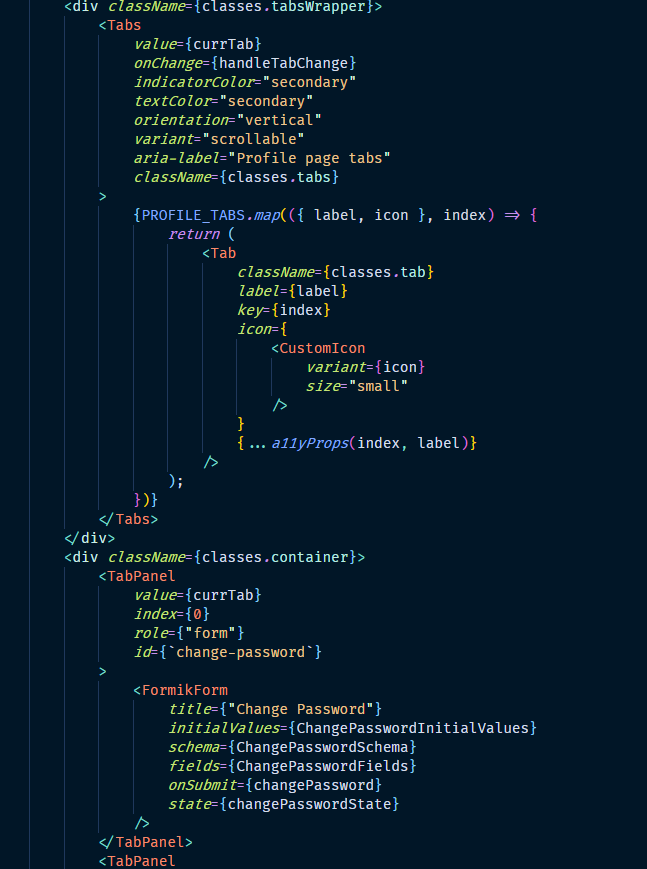
\includegraphics[scale=0.5]{implementacja/frontend/tabs}\\
	\caption{Przykład połączenia tabsów z tabpanelami}
	\label{fig:tabs}
\end{figure}

\subsection{Dialog}
\label{subsec:dialog}
Dialog to element zawierający tytuł, zawartość oraz akcje wyświetlający się nad innymi
 elementami strony przesłaniając je półprzeźroczystym czarnym tłem.
Informacje kontrolujące czy jest otwarty, czy zamknięty otrzymuje z zewnątrz tak samo, jak funkcje wywoływane na akcjach.
\begin{figure}[H]
	\centering
	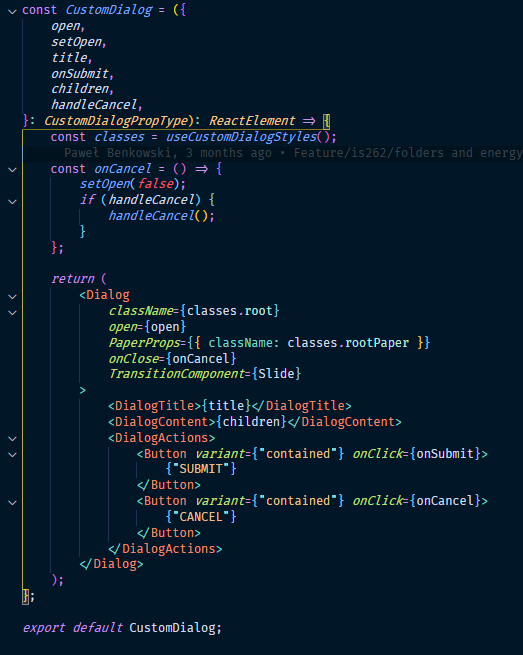
\includegraphics[scale=0.5]{implementacja/frontend/dialog}\\
	\caption{Implementacja dialogu}
	\label{fig:dialog}
\end{figure}

\subsection{Akordeon}
\label{subsec:accordion}
Akordeon to element zawierający nagłówek oraz ciało, który po kliknięciu otwiera się bądź zamyka.\\
Można również nadpisać jego akcje, umieszczając w tekście nagłówka guzik typu radio.
\begin{figure}[H]
	\centering
	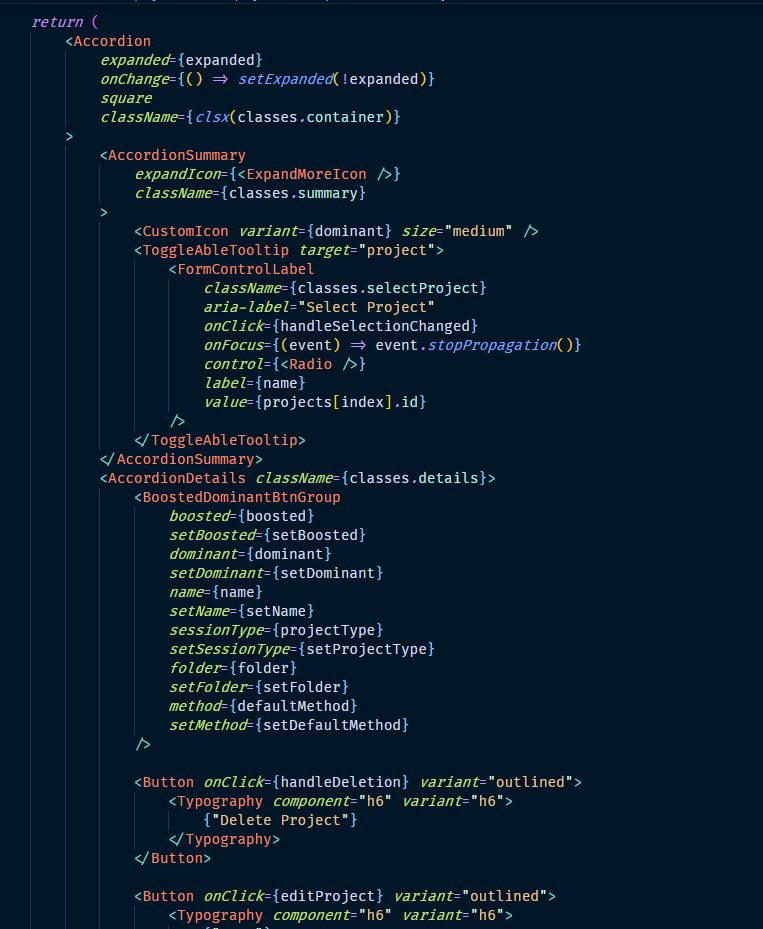
\includegraphics[scale=0.5]{implementacja/frontend/accordion}\\
	\caption{Implementacja akordeonu}
	\label{fig:accordion}
\end{figure}

\subsection{Style}
\label{subsec:style}
Zamiast tradycyjnych plików css korzystamy z CSS-in-JS - JSS gdzie style są tworzone z objektów JavaScript'owych.\\
Konkretnie wykorzystujemy implementacje tego podejścia z Material-UI i tworzymy nasze style od razu z dostępem do obiektu theme z biblioteki.
\begin{figure}[H]
	\centering
	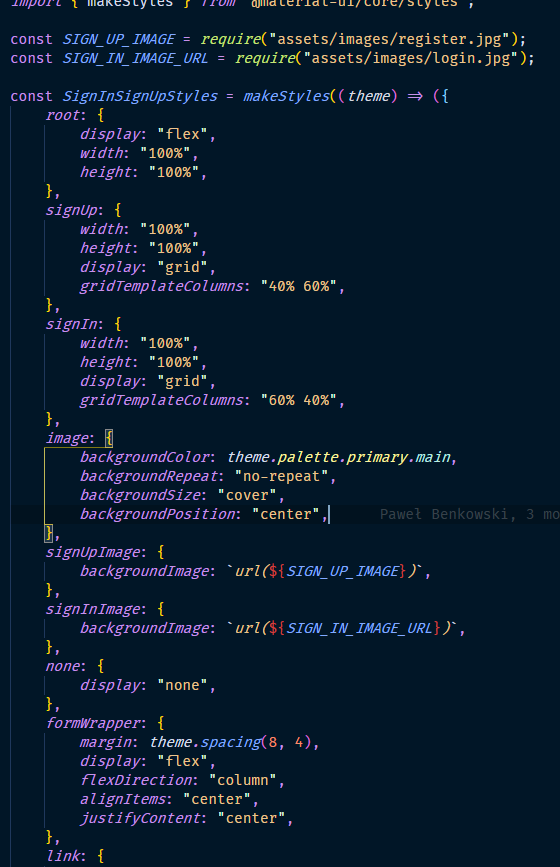
\includegraphics[scale=0.5]{implementacja/frontend/jss_styles}\\
	\caption{Przykład użycia makeStyles — implementacji JSS z Material-UI}
	\label{fig:jss_styles}
\end{figure}
\begin{figure}[H]
	\centering
	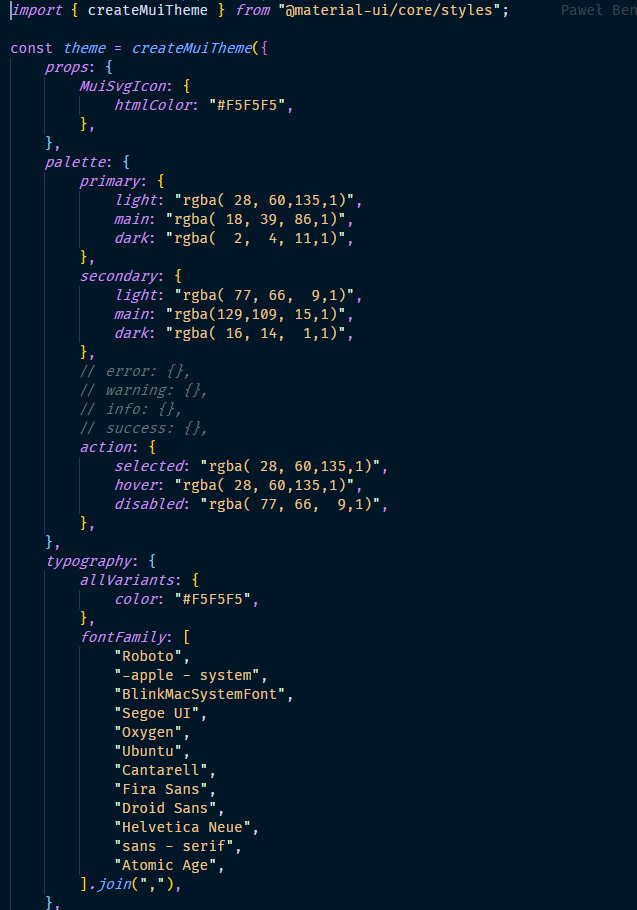
\includegraphics[scale=0.5]{implementacja/frontend/custom_theme}\\
	\caption{Obiekt theme z Material-UI}
	\label{fig:custom_theme}
\end{figure}

\subsection{Autoryzacja}
Wyświetla formularz \ref{subsec:forms} rejestracji lub logowania w zależności od kliknięcia „Already have an account?”, lub „Don't have and account?”.
Rejestracja zawiera pola:
\begin{itemize}
	\item Username na nazwe użytkownika.
	\item Email na mail, na który zostanie wysłany email potwierdzający konto.
	\item Password oraz Confirm password na hasło, oraz jego potwierdzenie.
\end{itemize}
Logowanie zawiera pola:
\begin{itemize}
	\item Username na nazwe użytkownika.
	\item Password na hasło danego konta.
\end{itemize}
Oraz przycisk do ponownego wysłania maila do weryfikacji.

\subsection{Gamitude Projects}
Zawiera komponent tabs przestawiony na rysunku nr \ref{subsec:tabs} wyświetlające foldery użytkownika, po kliknięciu pokazuje projekty w danym folderze z formie akordeonu \ref{subsec:accordion}.
W ciele akordeonu znajduje się formularz \ref{subsec:forms} do edycji projektu oraz guzik do jego usunięcia.\\
W nagłówku znajduje się guzik typu radio to zaznaczenia projektu dla czasomierza znajdującego się w panelu kontrolnym.

\subsection{Bullet Journal}
Komponent Bullet Journal Page został rozbity na kilka pomniejszych kompotentów.\\
 Komponenty Journal, Page oraz BulletTask odpowiadają za renderowanie odpowiedznio dzienników, stron oraz zadań z dziennika.
 BulletTask zawiera w sobie komponent TaskTile, będący przedstawiony w formie akordeonu, przedstawionym w podpunkcie nr \ref{subsec:accordion},
 którego zadaniem jest wyrenderowanie zawartości każdego zadania tj. możliwość zaznaczenia zadania, możliwość edycji zadania, możliwość usunięcia zadania i możliwość jego zakończenia.\\
 Journal oraz Page składają się z komponentu Tabs i TabPanel pokazanych w podpunkcie \ref{subsec:tabs}, które otrzymują dane na temat listy dzienników oraz stron z API.\\
 Komponenty AddJournalDialog i AddPageDialog są to komponenty typu dialog opisane w podrozdziale nr \ref{subsec:dialog},
 które suża do dodawania, edycji oraz usuwania dzienników, jak i stron z dzienników użytkownika.
 AddProjectTaskDialog służy jedynie do dodawania zadań.\\
\begin{figure}[H]
	\centering
	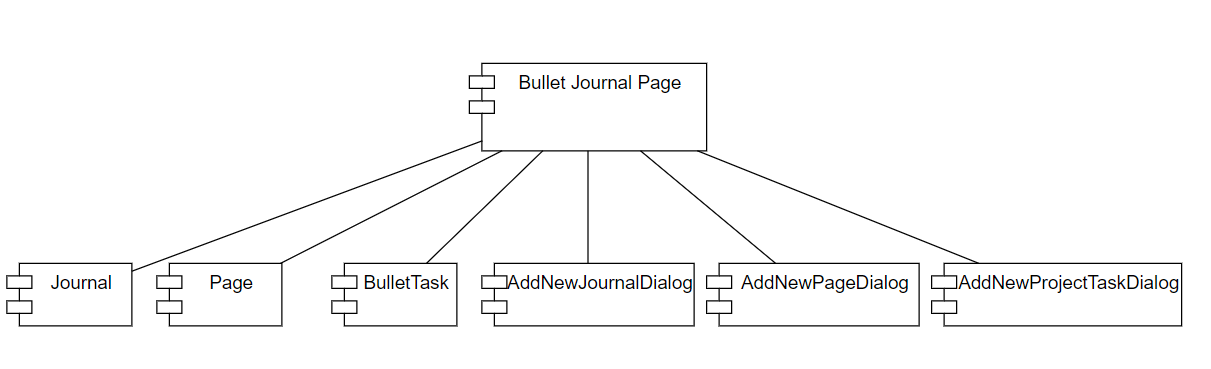
\includegraphics[scale=0.5]{implementacja/frontend/bullet_journal_diagram}\\
	\caption{Diagram komponentów zawartych w Bullet Journal}
	\label{fig:bullet_diagram}
\end{figure}
\begin{figure}[H]
	\centering
	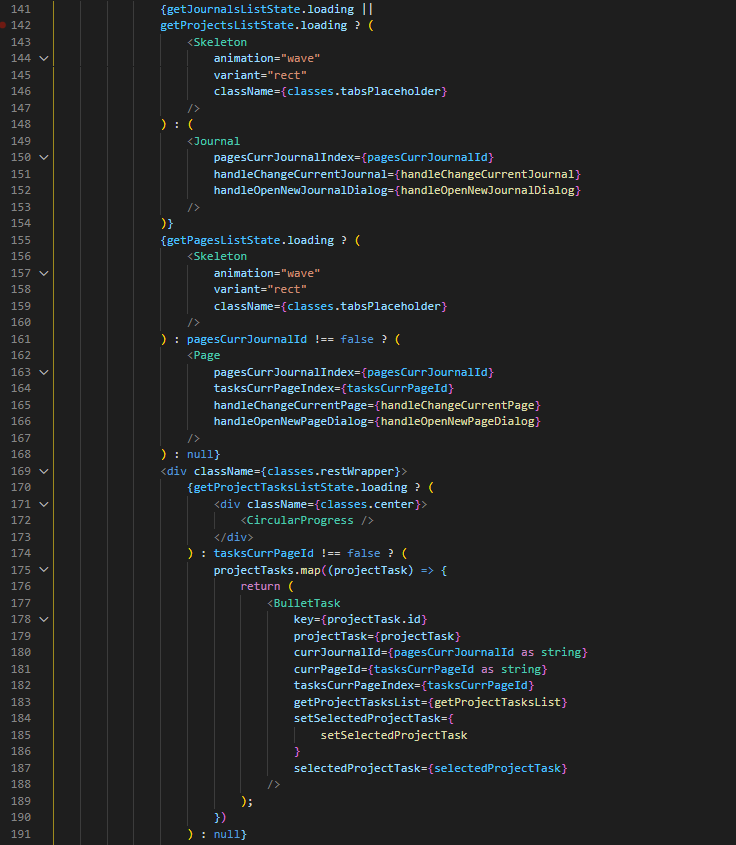
\includegraphics[scale=0.7]{implementacja/frontend/bullet_journal_division}\\
	\caption{Podział Bullet Journal Page na komponenty Journal, Page oraz Bullet Task}
	\label{fig:bullet_division}
\end{figure}

\subsection{Gamitude Themes}
Wyświetla dostępne rangi w formie kart po lewej natomiast mamy serie checkbox'ów do filtrowania wyników oraz paginacje.

\subsection{User Settings}
Składa się z tabsów \ref{subsec:tabs} zawierających formularze \ref{subsec:forms}:
\begin{itemize}
	\item Change Password z polami na potwierdzenie starego hasła, wprowadzenie nowego i potwierdzenie go.
	\item Change Email z polem na nowy email.
	\item Danger Zone z guzikiem do usunięcia konta — pojawi się modal z potwierdzeniem.
\end{itemize}

\section{Backend}
\label{subsec:bib_back}
\subsection{Struktura katalogów w projekcie}
\begin{figure}[H]
	\centering
	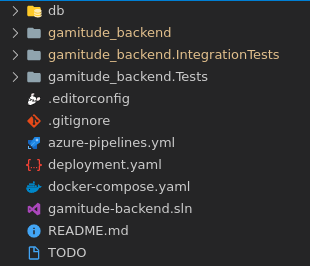
\includegraphics[scale=0.6]{implementacja/backend/struktura_folderow}\\
	\caption{Struktura całego projektu}
	\label{fig:folders}
\end{figure}
Projekt został podzielony na 3 podprojekty. Projekt gamitude\_backend zawiera główną implementację systemu.
Pozostałe 2 zostały stowrzone na potrzeby testowania.
\begin{figure}[H]
	\centering
	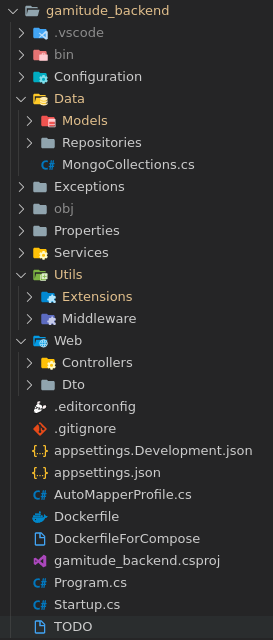
\includegraphics[scale=0.5]{implementacja/backend/struktura_folderow_gamitude_backend}\\
	\caption{Struktura głównego projektu}
	\label{fig:gamitude_struct}
\end{figure}
Główna implementacja systemu została podzielona na 3 warstwy tj. warstwa Web zawierająca kontrolery oraz ich kontrakty do komunikacji z warstwą prezentacji.
Warstwe serwisów zawierającą logike biznesową oraz warstwa Data, która przechowuje modele oraz ich repozytoria (klasy odpowiedzialne za komunikację z bazą danych).
Projekt zawiera również folder Utils, w którym przechowywane są funkcje pomocnicze. Autoryzacja w systemie została rozwiązana przy pomocy tokenów JWT.
Są one podpisane, dzięki temu można zweryfikować czy nie zostały zmodyfikowane. Można w nich przechowywać dane użytkownika np. jego unikalne Id.
\subsection{Skrócony diagram klas}
Rzut na całą implementację systemu z pominięciem klas pomocniczych i konfiguracyjnych.
\begin{figure}[H]
	\centering
	\rotatebox[origin=c]{270}{
	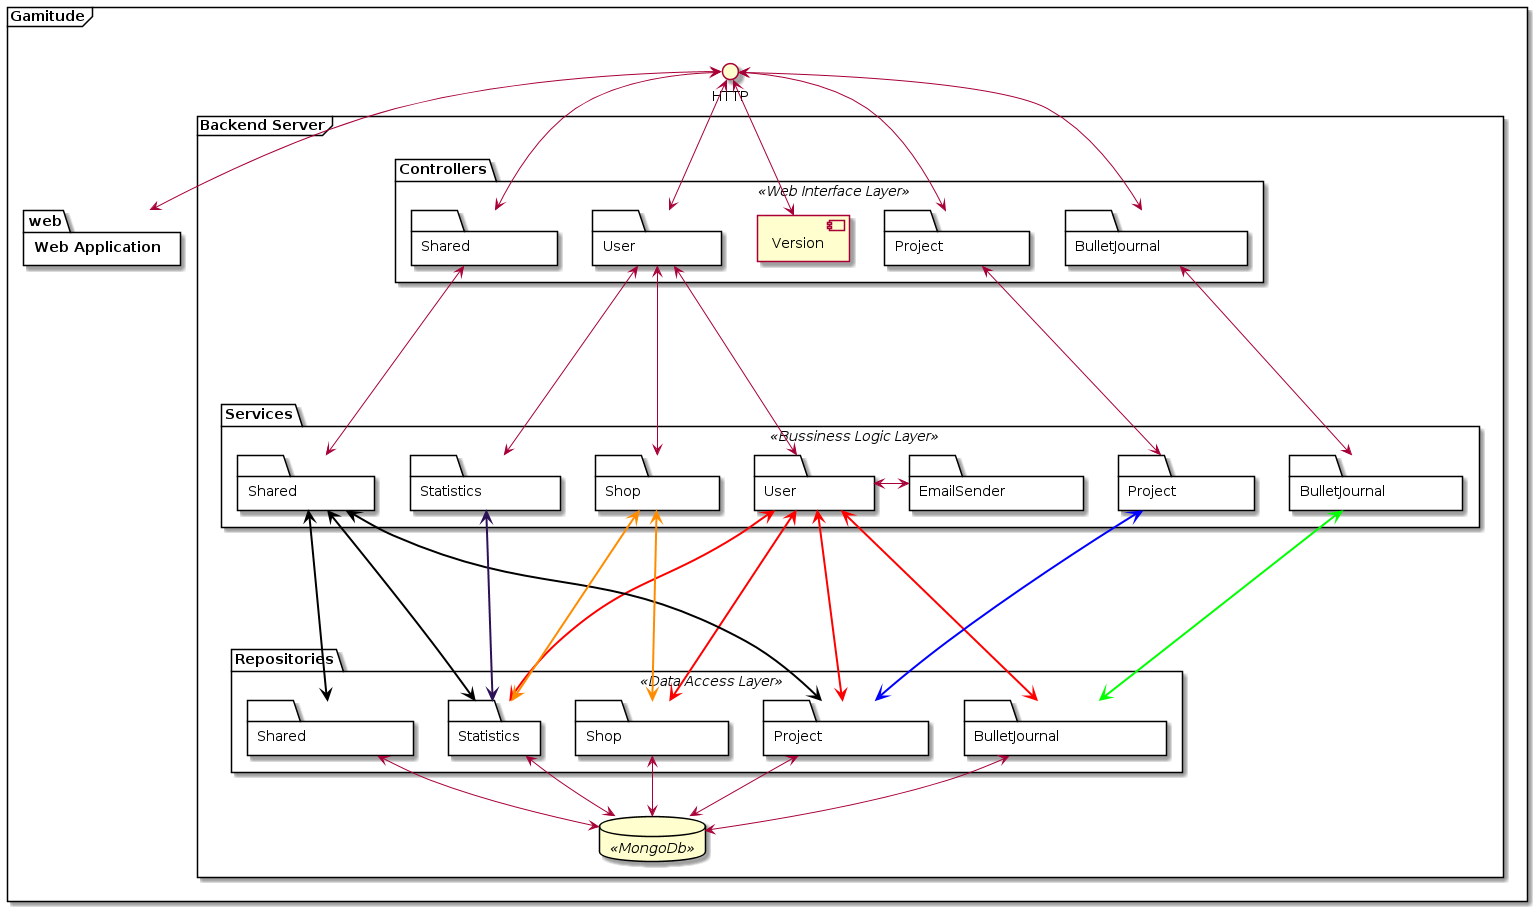
\includegraphics[scale=0.24]{implementacja/backend/gamitude_backend}}\\
	\caption{Skrócony diagram klas}
	\label{fig:gamitude_backend}
\end{figure}
\subsection{Endpointy API}
Wszystkie enpointy interfejsu Web API wraz z krótkim komentarzem przy każdym endpoincie.
Wygenerowane przy pomocy narzędza do dokumentowania API o nazwie swagger \cite{swagger}.
Pozwala ono na łatwe przedstawienie endpointów w formie graficznej przy minimalnej konfiguracji \cite{swagger-dotnet}.
Możliwe jest też szczegółowe udokumentowanie endpointów w kodzie.
Narzędzie jest bardzo przydatne, pozwala nawet na zaprojektownie wszystkich endpointów i poźniejsze wygenerowanie kodu.
Możliwe jest też wygenerowanie sobie klienta do konsumowaniu jakiegoś API.
\begin{figure}[H]
	\centering
	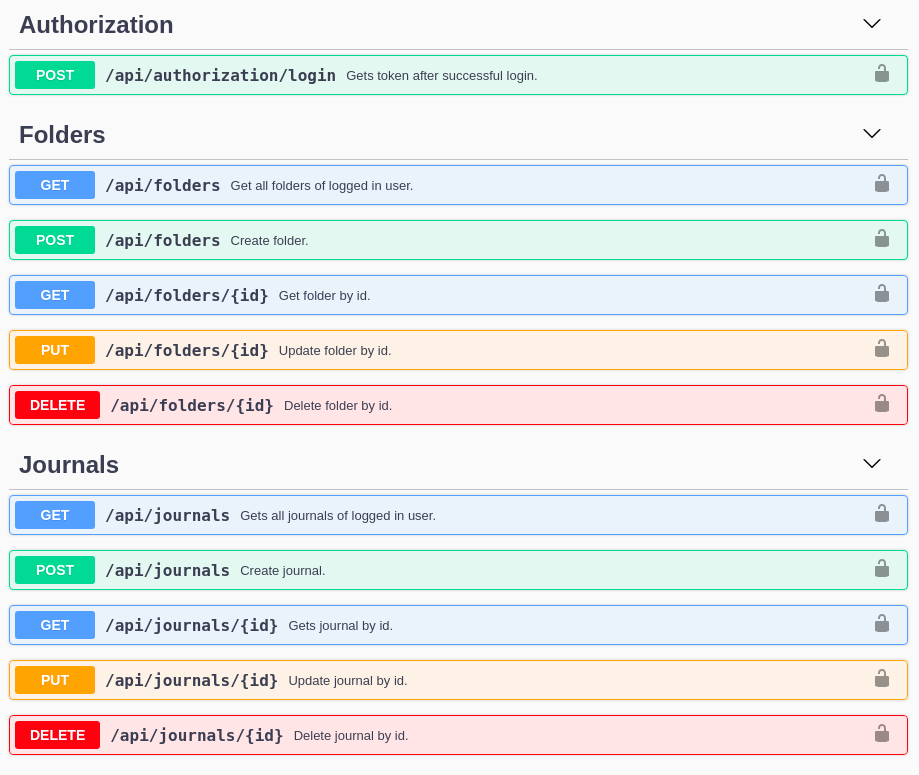
\includegraphics[scale=0.5]{implementacja/backend/auth_folders_journals_api}\\
	\caption{Enpointy Api}
	\label{fig:auth_folders_journals_api}
\end{figure}
\begin{figure}[H]
	\centering
	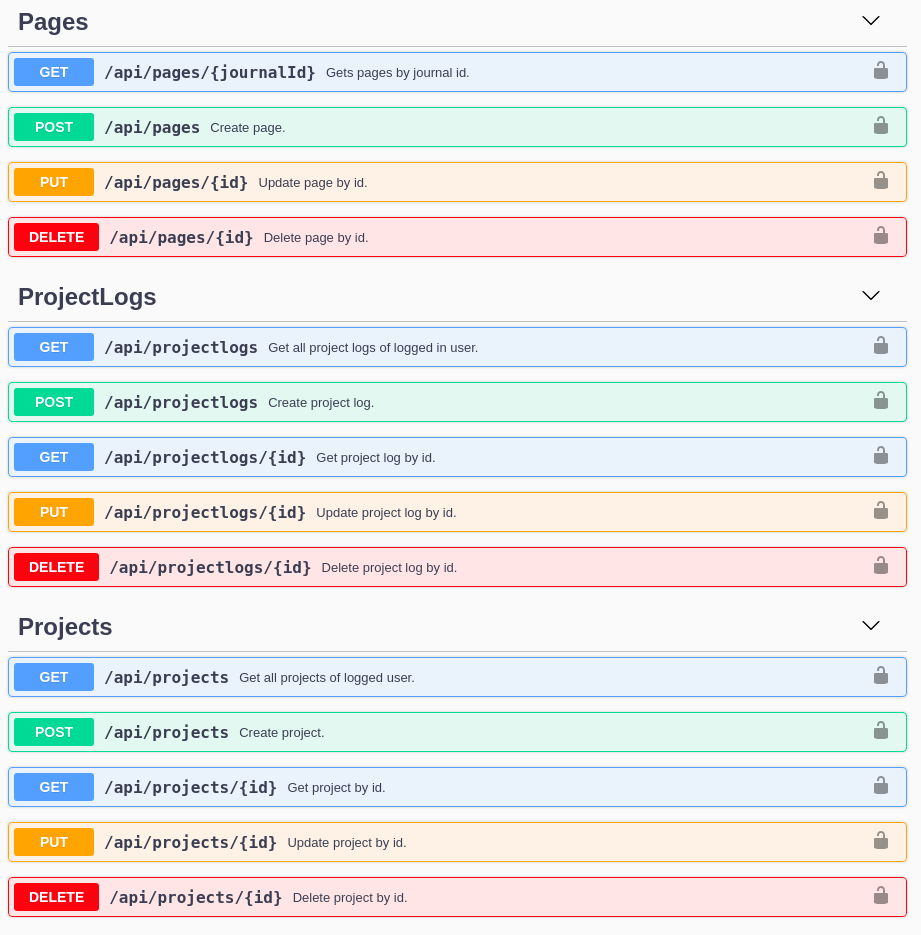
\includegraphics[scale=0.5]{implementacja/backend/pages_projectLogs_projects_api}\\
	\caption{Enpointy Api}
	\label{fig:pages_projectLogs_projects_api}
\end{figure}
\begin{figure}[H]
	\centering
	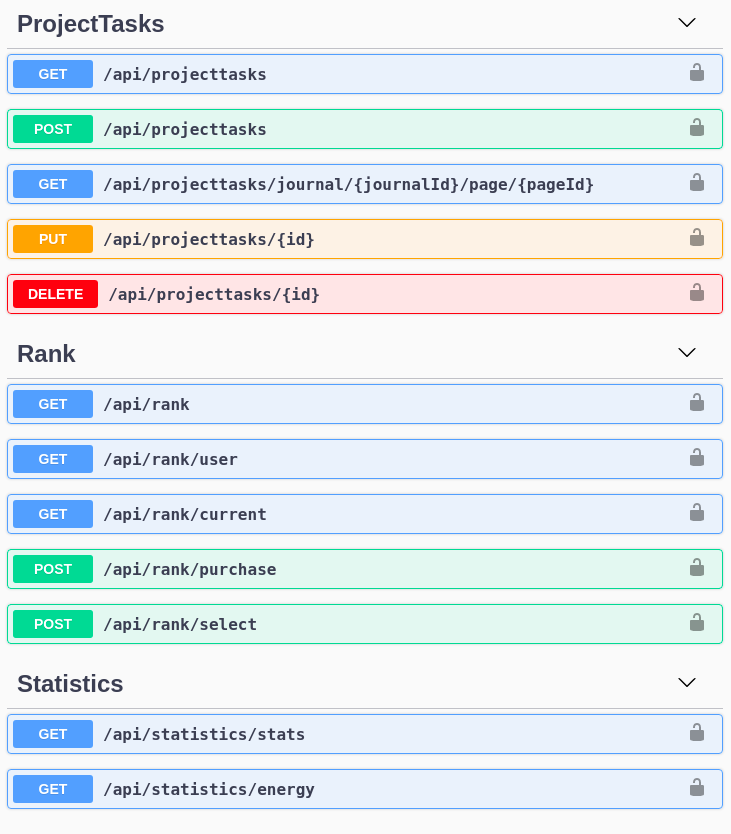
\includegraphics[scale=0.5]{implementacja/backend/projectTasks_rank_statistics_api}\\
	\caption{Enpointy Api}
	\label{fig:projectTasks_rank_statistics_api}
\end{figure}
\begin{figure}[H]
	\centering
	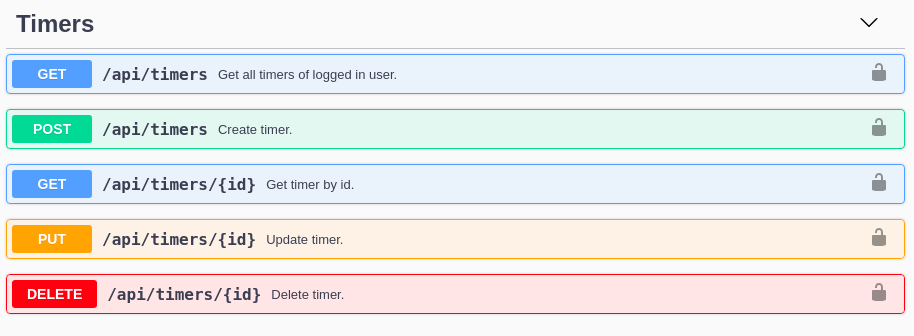
\includegraphics[scale=0.5]{implementacja/backend/timers_api}\\
	\caption{Enpointy Api}
	\label{fig:timers_api}
\end{figure}
\begin{figure}[H]
	\centering
	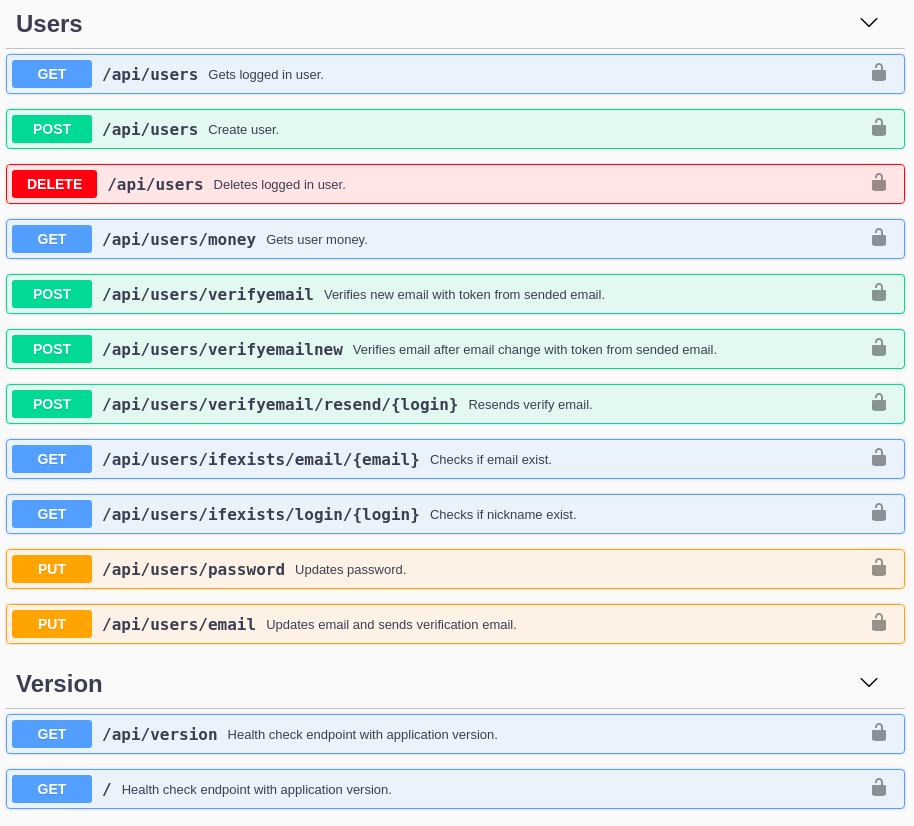
\includegraphics[scale=0.5]{implementacja/backend/users_api}\\
	\caption{Enpointy Api}
	\label{fig:users_api}
\end{figure}
\subsection{Baza danych}
Wykorzystana baza mongo dzięki swojej elastyczności pozwoliła na łatwą edycję struktury bazy szczególnie w rozwijającej się aplikacji.
Wystarczyło zmienić model w klasie odpowiedzialnej za dany model i podczas dodawania nowego obiektu do bazy był on tworzony automatycznie.
Baza Mongo nie posiada silnie wiążących relacji. 
Nie przeszkadza to w tworzeniu własnych, szczególnie w przypadku kiedy ilośc danych przekraczałaby wielkość maksymalną dokumentu tzn. 13 MB.
Takie relacje zostały stworzone w przypadku tokenów, statystyk, dziennych energi, czasomierzy (timer), projektów i ich logów. Relacja też została zastosowana do przetrzymywania identyikatorów zakupionych rang, gdyż są one takie same dla wszystkich i niepotrzebne jest przechowywanie ich kopii.
W logu projektu przechowujemy kopie projektu, aby był on dokładnych odzwierciedleniem projektu w momencie kończenia sesji. W naszej finalnej wersji modelu bazy danych zauważyliśmy pare błędów, które zaplanowane są do poprawy w nastepnej wersji projektu.
Przeniesienie statystyk do obiektu użytkownika (wynika to z faktu, że kiedyś statystyki były per dzień). Przeniesienie czasomierzy (timer) do obiektu użytkownika. Ponowne przemyślenie struktury folders, projects, aby skomasować je w jeden obiekt.
Finalne modele bazy danych.
\begin{figure}[h]
	\centering
	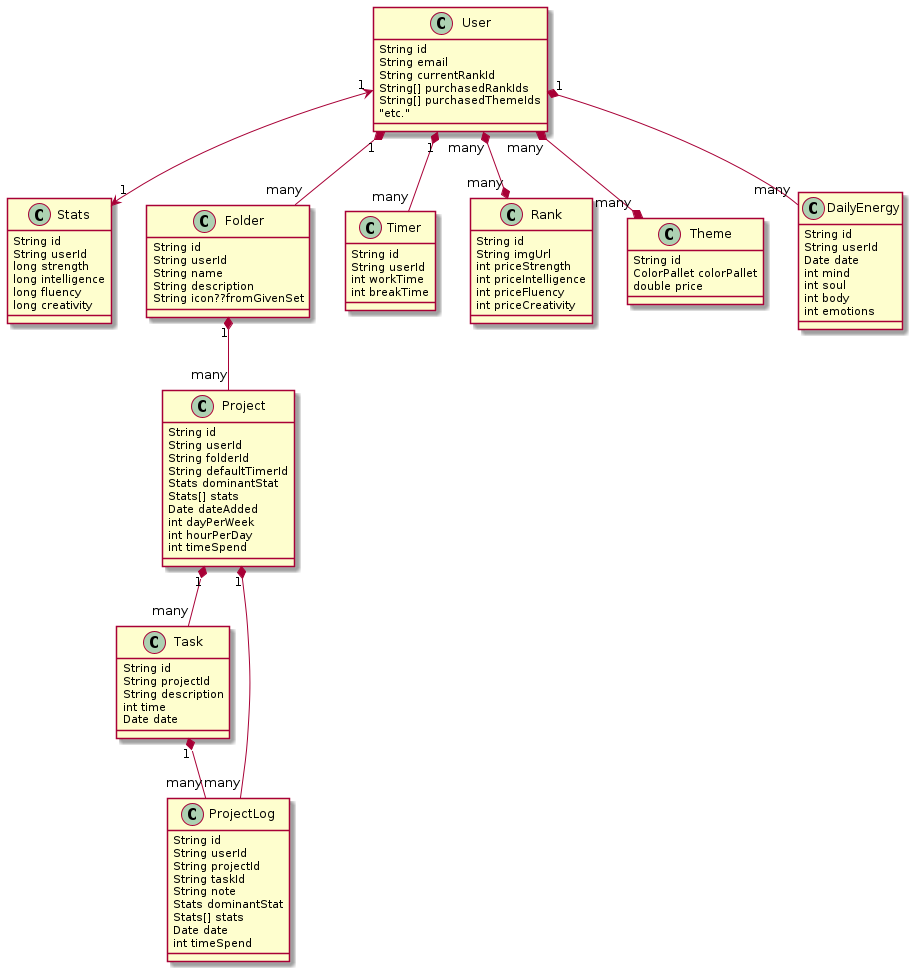
\includegraphics[width=\textwidth, height=10cm]{gamitude_database_model}\\
	\caption{Schemat bazy danych}
	\label{fig:db}
\end{figure}
\subsection{Utills}
Przykład klasy extension rysunek nr \ref{fig:gamitude_extension} oraz  middleware rysunek nr \ref{fig:gamitude_middleware}.
Używane one są do konfiguracji całej aplikacji w bardziej przejrzysty sposób rysunek nr \ref{fig:gamitude_services_startup} oraz nr \ref{fig:gamitude_pipeline_startup}.
\begin{figure}[H]
	\centering
	\includegraphics[scale=0.35]{implementacja/backend/przykład_extension}\\
	\caption{Przykład extension}
	\label{fig:gamitude_extension}
\end{figure}
\begin{figure}[H]
	\centering
	\includegraphics[scale=0.35]{implementacja/backend/przykład_middleware}\\
	\caption{Przykład middleware}
	\label{fig:gamitude_middleware}
\end{figure}
\begin{figure}[H]
	\centering
	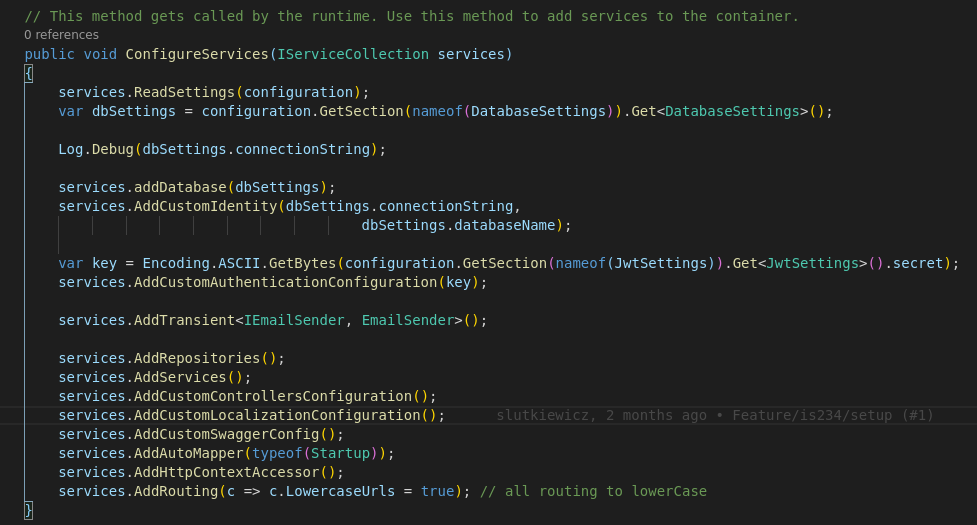
\includegraphics[scale=0.3]{implementacja/backend/register_services_startup}\\
	\caption{Rejestracja serwisów w startup.cs}
	\label{fig:gamitude_services_startup}
\end{figure}
\begin{figure}[H]
	\centering
	\includegraphics[scale=0.3]{implementacja/backend/przykład_pipeline_startup}\\
	\caption{Konfiguracja http pipeline w startup.cs}
	\label{fig:gamitude_pipeline_startup}
\end{figure}
\subsection{Kontrolery}
Klasy odpowiedzialne za:
\begin{itemize}
	\item Komunikacje z warstwą prezentacji protokołem HTTP.
	\item Przetworzenie kontraktu na model, jeżeli konieczne.
	\item Zainicjalizowania wykonania logiki biznesowej.
	\item Zwrócenia odpowiedniego kontraktu, jeżeli to konieczne.
\end{itemize}
Przykładowe metody kontrolerów.
\begin{figure}[H]
	\centering
	\includegraphics[scale=0.3]{implementacja/backend/przykład_get}\\
	\caption{Metoda GET w kontrolerze}
	\label{fig:przykład_get}
\end{figure}
\begin{figure}[H]
	\centering
	\includegraphics[scale=0.3]{implementacja/backend/przykład_post}\\
	\caption{Metoda POST w kontrolerze}
	\label{fig:przykład_post}
\end{figure}
\begin{figure}[H]
	\centering
	\includegraphics[scale=0.3]{implementacja/backend/przykład_put}\\
	\caption{Metoda PUT w kontrolerze}
	\label{fig:przykład_put}
\end{figure}
\begin{figure}[H]
	\centering
	\includegraphics[scale=0.3]{implementacja/backend/przykład_delete}\\
	\caption{Metoda DELETE w kontrolerze}
	\label{fig:przykład_delete}
\end{figure}
Przykładowe kontrakty.
\begin{figure}[H]
	\centering
	\includegraphics[scale=0.5]{implementacja/backend/przykład_timer_dto_get}\\
	\caption{Kontrakt zwracanego timera}
	\label{fig:przykład_timer_dto_get}
\end{figure}
\begin{figure}[H]
	\centering
	\includegraphics[scale=0.5]{implementacja/backend/przykład_timer_dto_create}\\
	\caption{Kontrakt do tworzenia timera}
	\label{fig:przykład_timer_dto_create}
\end{figure}
\begin{figure}[H]
	\centering
	\includegraphics[scale=0.5]{implementacja/backend/przykład_timer_dto_update}\\
	\caption{Kontrakt do edycji timera}
	\label{fig:przykład_timer_dto_update}
\end{figure}
Konfiguracja mappera do przetwarzania obiektów pomiędzy kontraktami.
\begin{figure}[H]
	\centering
	\includegraphics[scale=0.5]{implementacja/backend/przykład_mappera}\\
	\caption{Konfiguracja mappera obiektów timera}
	\label{fig:przykład_mappera}
\end{figure}


\subsection{Serwisy}
Klasy odpowiedzialne przechowanie logiki biznesowej np. dodatkową obróbkę danych bądź bardziej skomplikowane operacje na wielu repozytoriach.
Pozwala to na odzielenie logi od bazy danych w przypadku późniejszej jej zmiany, wystarczy podmienić repozytorium, które implementuje dany interfejs.
Przykład serwisu
\begin{figure}[H]
	\centering
	\includegraphics[scale=0.4]{implementacja/backend/przykład_timer_service}\\
	\caption{Serwis timera}
	\label{fig:przykład_timer_service}
\end{figure}
\subsection{Repozytoria}
Klasa odpowiedzialna za komunikację z bazą danych przechowuje ona logike odczytu zapisu. 
Przykład repozytorium oraz jego interfejsu
\begin{figure}[H]
	\centering
	\includegraphics[scale=0.4]{implementacja/backend/przykład_timer_irepo}\\
	\caption{Interfejs repozytorium timera}
	\label{fig:przykład_timer_irepo}
\end{figure}
\begin{figure}[H]
	\centering
	\includegraphics[scale=0.4]{implementacja/backend/przykład_timer_repo}\\
	\caption{Repozytorium timera}
	\label{fig:przykład_timer_repo}
\end{figure}
\subsection{Modele}
Klasy odpowiedzialne za przechowywanie struktury modeli, które są odpowiednikami znajdującymi się w bazie danych.
\begin{figure}[H]
	\centering
	\includegraphics[scale=0.5]{implementacja/backend/przykład_timer_model}\\
	\caption{Model timera}
	\label{fig:przykład_timer_model}
\end{figure}
\begin{figure}[H]
	\centering
	\includegraphics[scale=0.5]{implementacja/backend/przykład_timer_model_count}\\
	\caption{Model CountDownInfo osadzonego w klasie Timer}
	\label{fig:przykład_timer_model_count}
\end{figure}

\subsection{Wykorzystane biblioteki}
\begin{itemize}
	\item AutoMapper – mapowanie obiektów pomiędzy klasami.
	\item Microsoft AspNetCore Authentication JwtBearer – weryfikowanie JWT pipelin'a autentykowania i autoryzacji użytkownika.
	\item System IdentityModel Tokens Jwt – manipulacja tokenami JWT.
	\item SendGrid – wysyłanie maili.
	\item Swashbuckle AspNetCore – generowanie dokumentacji API.
	\item AspNetCore Identity Mongo AspNetCore – Zarządzanie użytkownikami.
	\item MongoDB Driver – Sterownik bazy danych Mongo.
	\item Serilog AspNetCore – Logger.
	\item NWebsec AspNetCore Middleware – Security HTTP headers.
\end{itemize}

\chapter {Historia sprintów}
\section {Rozpoznanie dziedzinowe}
\subsection {Założenia sprintu}
Każdy członek zespołu wybrał sobie pewien sposób na zarządzanie swoimi zadaniami w ciągu dnia w celu zbadania dziedziny problemu.
\subsection {Wykonane zadania}
Paweł: Używanie metodologi Pomodoro i Ultradian rhythm do codziennych zadań. Przerabianie kursu React.\\
Robert: Rozplanowywanie zadań za pomocą GTD (Getting Things Done)\\
Stanisław: Zapoznanie się i zastosowanie Bullet Journal'a oraz szukanie alternatyw dla narzędzi do dokumentowania projektu (Enterprise Architect, Github).\\
\subsection {Napotkane problemy}
Brak zastępcy dla programu Enterprise Architect. Spór dotyczący wyboru Azure Repos a Github'em.

\section {Wstępna dokumentacja}
\subsection {Założenia sprintu}
Podczas sprintu, zespół miał za zadanie wytworzyć wstępne dokumenty DZW i SWS oraz znalezienie sposobu na kontrolę wersji w EA.
\subsection {Wykonane zadania}
Paweł: Wytworzenie wstępnej wersji dokumentu DZW. Przerabianie kursu React.\\
Robert: Wytworzenie wstępnej wersji dokumentu SWS.\\
Stanisław: Rozpoznanie dotyczące kontroli wersji w EA. Rozpoznanie architektury mikro serwisów oraz projektowania jej.\\
\subsection {Napotkane problemy} 
Kontrola wersji w EA dostępne tylko po wykupieniu licencji.

\section {Use Case + WPP}
\subsection {Założenia sprintu}
Przygotowanie pierwszych diagramów Use Case. Wytworzenie dokumentu WPP.
\subsection {Wykonane zadania}
Paweł: Wytworzenie paru Use Case'ów w programie EA. Przerabianie kursu React.\\
Robert: Stworzenie dokumentu WPP oraz jednego z Use Case'ów.\\
Stanisław: Wytworzenie paru Use Case'ów w programie EA.\\
\subsection {Napotkane problemy}
Brak napotkanych problemów.

\section {Dalsza praca przy SWS}
\subsection {Założenia sprintu}
Doprecyzowanie wymagań systemowych oraz niefunkcjonalnych w dokumencie SWS. Podjąć decyzję odnośnie do wyboru architektury systemu.
\subsection {Wykonane zadania}
Zespół: Wspólna praca nad SWS oraz wybranie architektury mikroserwisowej dla systemu.\\
Paweł: Przerabianie kursu React.\\
\subsection {Napotkane problemy}
Brak napotkanych problemów.

\section {Przygotowanie narzędzi do tworzenia systemu}
\subsection {Założenia sprintu}
Znalezienie i skonfigurowanie platformy do komunikacji zespołu, stworzenie repozytoriów dla każdego mikro serwisu oraz przygotowanie wstępnego mockup'u UI dla systemu.
\subsection {Wykonane zadania}
Paweł: Stworzenie pierwszego mockup'u UI dla systemu. Przerabianie kursu React. \\
Stanisław: Stworzenie repozytoriów dla wszystkich mikro serwisów oraz przygotowanie platformy Slack do komunikacji zespołu.\\
\subsection {Napotkane problemy}
Rozmowy grupowe na platformie Slack były płatne, więc musieliśmy znaleźć alternatywę dla domyślnych rozmów.

\section {Diagramy funkcjonalności, wymagania bazy danych oraz responsywne rozłożenie strony}
\subsection {Założenia sprintu}
Każdy z członków zespołu stworzy diagram funkcjonalności dla swojego mikro serwisu, który pomoże w określeniu wymagań funkcjonalnych. Utworzony zostanie diagram wymagań dla bazy danych oraz wykres Gantt’a i wstępne ułożenie poszczególnych komponentów na stronie.
\subsection {Wykonane zadania}
Zespół: Tworzenie wykresu Gantt'a.\\
Paweł: Utworzenie responsywnego rozłożenia strony. \\
Robert: Stworzenie diagramu funkcjonalności. \\
Stanisław: Stworzenie diagramu funkcjonalności oraz bazy danych.\\
\subsection {Napotkane problemy}
Znalezienie darmowego narzędzia dla wykresu Gantt'a.

\section {Diagramy klas i nawigacja strony}
\subsection {Założenia sprintu}
Członkowie zespołu odpowiedzialni za backend projektu wykonają diagramy klas dla swoich serwisów, utworzą struktury plików dla poszczególnych mikro serwisów, przygotują routing dla nich. Zostanie stworzona nawigacja strony.
\subsection {Wykonane zadania}
Robert i Stanisław: Utworzenie diagramu klas dla mikro serwisów oraz struktury plików dla nich.\\
Paweł: Implementacja nawigacji strony. \\
Stanisław: Stworzenie routingu dla mikro serwisu projektów.\\
\subsection {Napotkane problemy}
Robert nie przygotował routingu.

\section {Diagram sekwencji oraz statystyki i energie na stronie}
\label{sec:system_statystyk}
\subsection {Założenia sprintu}
Zostanie utworzony diagram sekwencji pozwalający zobrazować przepływ danych w projekcie. Utworzone zostaną widoki statystyk i energii na stronie.
\subsection {Wykonane zadania}
Robert i Stanisław: Utworzenie diagramu sekwencji.\\
Paweł: Implementacja widoków statystyk i energii. \\
Robert: Utworzono routing w mikro serwisie rang.\\
Stanisław: Modyfikacja modelu projektów w bazie danych.\\
\subsection {Napotkane problemy}
Brak napotkanych problemów.

\section {Algorytmy oraz rangi na stronie}
\label{sec:system_zarzadzania_energia_uzytkownika}
\subsection {Założenia sprintu}
Stworzenie algorytmów odpowiedzialnych za przyznawanie rangi oraz za wzrost lub spadek energii. Zaimplementowanie struktury bazy danych zgodnej z dokumentacją oraz utworzenie rang na frontend'ie.
\subsection {Wykonane zadania}
Paweł: Implementacja widoków rang. \\
Robert: Algorytm przyznawania rang i statystyk.\\
Stanisław: Algorytm wzrostu i spadku energii. Implementacja struktury bazy danych.\\
\subsection {Napotkane problemy}
Brak napotkanych problemów.

\section {Firebase, Heroku, projekty}
\label{sec:system_zarzadzania_projektami_uzytkownikow}
\subsection {Założenia sprintu}
Utworzenie konta firebase dla projektu, schematów modeli bazy danych dla mikro serwisów, przeniesienie bazy danych na platformę Heroku, utworzenie wyglądu projektów na frontendzie.
\subsection {Wykonane zadania}
Robert i Stanisław: Stworzenie schematów modeli bazy danych dla mikro serwisów.\\
Paweł: Implementacja widoków projektów. Refaktoryzacja dotychczasowego kodu. \\
Stanisław: Przeniesienie bazy danych na platformę Heroku. Utworzenie konta firebase dla projektu.\\
\subsection {Napotkane problemy}
Modele rang i workflow niezgodne z założeniami, do poprawy w następnym sprincie.

\section {Firebase autoryzacja, API refactor}
\subsection {Założenia sprintu}
Dodanie rang do bazy danych, serwisu firebase do projektu, funkcji tworzenia użytkownika przez firebase, refaktoryzajca serwisów workflow i projektów, utworzenie strony logowania i rejestracji na frontendzie oraz poprawienie wyglądu projektów.
\subsection {Wykonane zadania}
Robert i Stanisław: Poprawa modeli rang i workflow.\\
Paweł: Utworzenie strony logowania i rejestracji na frontendzie oraz poprawienie wyglądu projektów, dodanie serwisu firebase do projektu oraz funkcji tworzenia użytkownika przez firebase.\\
Robert: Dodanie rang do bazy danych.\\
Stanisław: Refaktoryzajca serwisów workflow i projektów. Dodanie API do przyjmowania poświęconego czasu.\\
\subsection {Napotkane problemy}
Algorytmy niedostosowane do działania w czasie. Poprawa na następny tydzień.

\section {Integracja}
\subsection {Założenia sprintu}
Ukończono prace nad algorytmami związanymi z przyznawaniem rang oraz zmianą energii, dodanie wszystkich działających endpoint’ów do serwisu frontend'owego.
\subsection {Wykonane zadania}
Robert i Stanisław: Dostosowanie algorytmów do wymagań. \\
Paweł: Integracja z API.\\
Stanisław: Dodanie obsługi błędów związanych z bazą danych. \\
\subsection {Napotkane problemy}
Problem z integracją frontend'u z API.

\section {Prezentacja i demo}
\subsection {Założenia sprintu}
Utworzenie prezentacji projektu oraz pokazowego dema działania aplikacji.
\subsection {Wykonane zadania}
Robert: Wykonanie pokazowego dema. \\
Paweł: Stworzenie prezentacji.\\
\subsection {Napotkane problemy}
Przez problemy z integracją frontend'u z API, część projektu musiała zostać postawiona na mockup'ach.

\section {Zmiana technologii na backendzie, retrospekcja}
\subsection {Założenia sprintu}
Przyjrzenie się powstałemu już systemowi i wyznaczenie kierunku dalszych prac.
\subsection {Wykonane zadania}
Zespół: Ustalenie zmiany technologi backend'owej na C\#, zaakceptowanie pomysłu na utworzenie sklepu z motywami dla aplikacji, wspólna decyzja o zrezygnowaniu z firebase'a.\\
Paweł: Utworzenie nowego formularza logowania i rejestracji bez firebase'a.\\
Stanisław: Rozpoczęcie prac nad przerabianiem serwisów z NodeJs na C\#, praca nad serwisem autoryzacji użytkownika, przystosowanie chmury do pracy z technologią .NET, wyeksportowanie obecną bazę danych do pliku lokalnego w razie zmiany bazy.\\
\subsection {Napotkane problemy}
Brak napotkanych problemów.

\section {Festiwal pomysłów i mockup'y}
\subsection {Założenia sprintu}
Szukanie nowych pomysłów na funkcjonalności. Stworzenie mockup'ów dla strony głównej oraz Bullet Journal'a. 
\subsection {Wykonane zadania}
Paweł: Elastic habits, Just 5, flow state, Energy asistant, system osiągnięć czy system rankingu między graczami.\\
Robert: Stworzenie mockup'u strony głównej oraz Bullet Journal'a.\\
Stanisław: Przeniesienie bazy danych z Heroku do chmury mongo atlas. Pomysł na zbieranie informacji o użytkownikach dla późniejszej sprzedaży.\\
\subsection {Napotkane problemy}
Brak napotkanych problemów.

\section {Festiwal pomysłów ciąg dalszy}
\subsection {Założenia sprintu}
Zakończenie prac nad serwisem projektów oraz zaczęcie prac nad serwisem rang. Dalsze szukanie pomysłów.
\subsection {Wykonane zadania}
Paweł: skills, wybieranie innego zadania jako przerwy, tworzenie statystyk użytkownika z danych zadań.\\
Stanisław: Zakończono pracę nad serwisem projektów oraz zaczęto nad serwisem rang.\\
\subsection {Napotkane problemy}
Brak napotkanych problemów.

\section {Autoryzacja i budowanie bibliografii}
\label{sec:system_autoryzacji_uzytkownika}
\subsection {Założenia sprintu}
Połączenie frontend'u z serwisem logowania i rejestracji. Zbudowanie podstawowej bibliografii.
\subsection {Wykonane zadania}
Paweł i Stanisław: Połączenie frontend'u z przepisanym serwisem.\\
Robert: Zebranie danych dotyczących źródeł informacji do bibliografii.\\
Stanisław: Początek przenoszenia projektów z Heroku do chmury Google.\\
\subsection {Napotkane problemy}
Brak napotkanych problemów.

\section {Smartwatch'e i MBTI}
\subsection {Założenia sprintu}
Szukanie informacji na temat wykorzystania smartwatch'y w aplikacji. Rozpoznanie w zakresie różnych typów użytkowników systemu. 
\subsection {Wykonane zadania}
Paweł i Robert: Wykonanie badania MBTI.\\
Stanisław: Przenoszenie kolejnych mikro serwisów do chmury Google'a. Stworzenie mikro serwisu od autoryzacji. Pomysł na integracje aplikacji z Google Calendar.\\
\subsection {Napotkane problemy}
Brak napotkanych problemów.

\section {Odnowienie dokumentacji i bezpieczeństwo}
\subsection {Założenia sprintu}
Zebranie całej starej dokumentacji w jedno miejsce. Zapewnienie bezpieczeństwa aplikacji.  
\subsection {Wykonane zadania}
Zespół: Modyfikacja dokumentu DZW.\\
Robert: Zebranie całej dokumentacji i wstawienie jej na platformę Github, napisanie streszczenia projektu.\\
Stanisław: Szukanie informacji na temat certyfikatu SSL oraz równoważenia obciążenia\\
\subsection {Napotkane problemy}
Koszt load balancer'a w chmurze Google'a przewyższa koszt jednej maszyny wirtualnej.


\section {Autoryzacja, dokumentacja}
\subsection {Założenia sprintu}
Poprawa bibliografii, zebranie historii sprintów, poprawa wyglądu systemu autoryzacji użytkownika po stronie frontend'u.
\subsection {Wykonane zadania}
Robert: Stworzenie bibliografii zgodnie z zaleceniami dziekana, skończenie spisywanie historii sprintów do obecnego stanu, wstępne poprawki do dokumentu SWS.\\
Paweł: Implementacja poprawek systemu autoryzacji użytkownika po stronie frontend'u.\\
Stanisław: Research na temat architektury systemu.\\
\subsection {Napotkane problemy}
Brak napotkanych problemów.

\section {Końcowe prace nad przepisanymi serwisami}
\subsection {Założenia sprintu}
Zintegrowanie serwisu projektów, uaktualnienie dokumentów o uwagi promotora, kończenie prac nad serwisem statystyk i energii.
\subsection {Wykonane zadania}
Paweł: Integracja serwisu projektów, walidacja wprowadzonych danych na frontend.\\
Robert: Uzupełnienie DZW o nowe funkcjonalności, stworzenie dokumentu SWS oraz ulepszenie o uwagi promotora.\\
Stanisław: Końcowe prace nad serwisem statystyk i energii, naprawianie błędów w stworzonych serwisach.\\
\subsection {Napotkane problemy}
Brak napotkanych problemów.

\section {Integracja i LaTeX}
\subsection {Założenia sprintu}
Integracja zakończonych mikro serwisów, przygotowania do przepisania dokumentacji na latex.
\subsection {Wykonane zadania}
Robert: Wstępna wersja widoku Gamitude Themes, zbieranie informacji na temat języka do tworzenia dokumentacji LaTeX.\\
Paweł: Obsługa błędów dla projektów, integracja serwisu statystyk i energii.\\
Stanisław: skończenie serwisu statystyk, czytanie o mikro serwisach, prace nad cron'em.\\
\subsection {Napotkane problemy}
Brak napotkanych problemów.

\section {Przepisywanie dokumentacji}
\subsection {Założenia sprintu}
Stworzenie domyślnego dokumentu dla pracy oraz rozpoczęcie prac nad przepisywaniem pozostałych dokumentów.
\subsection {Wykonane zadania}
Robert: przerabianie dokumentów na latex.\\
Paweł: zbieranie informacji na temat połączenia kalendarza i Bullet Journal'a.\\
Stanisław: przerabianie kursu o identity serwer 4.\\
\subsection {Napotkane problemy}
Brak napotkanych problemów.


\section {Podpowiedzi i naprawa błędów}
\subsection {Założenia sprintu}
Dodanie podpowiedzi dla użytkownika, by ułatwić zapoznawanie się z systemem. Naprawa błędów w przeliczaniu statystyk
\subsection {Wykonane zadania}
Robert: dodanie karty projektów w latex.\\
Paweł: Stworzenie podpowiedzi dla użytkowników na stronie. \\
Stanisław: Poprawa błędów w obliczaniu statystyk.  \\
\subsection {Napotkane problemy}
Brak napotkanych problemów.

\section {DZW i integracja rang}
\subsection {Założenia sprintu}
Zintegrowanie przepisanego systemu rang, przepisanie dokumentu DZW na LaTeX.
\subsection {Wykonane zadania}
Robert: Dodanie DZW do latex dokumentu, przerobienie bibliografii.\\ 
Paweł: Dodanie więcej podpowiedzi do strony, dodawanie projektu przeniesione do modal'a, połączenie API rang z frontend'em.\\
Stanisław: Naprawiony system rang, dodanie load balancer'a do projektu jako swój własny serwis w Kubernetes'ie. Brak idealnego rozwiązania. \\
\subsection {Napotkane problemy}
Brak napotkanych problemów.

\section {SWS i nowe minutniki}
\label{sec:zarzadzanie_czasomierzem}
\subsection {Założenia sprintu}
Wstępna implementacja nowych minutników, zastosowanie certyfikatu SSL na stronie, przepisanie SWS do LaTeX.
\subsection {Wykonane zadania}
Robert: SWS przepisany do latex.\\
Paweł: Implementacja minutników flow state, just 5 i custom time. \\ 
Stanisław: Dodanie certyfikatu SSL.  \\
\subsection {Napotkane problemy}
Brak napotkanych problemów.

\section {Strona główna i przerwy}
\subsection {Założenia sprintu}
Wstępna implementacja przerw, stworzenie pierwszej wersji strony głównej z użyciem parallax.
\subsection {Wykonane zadania}
Robert: Pierwsza wersja strony głównej w parallax.\\
Paweł: Rozpoczęcie implementacji przerw.\\
Stanisław: Dodanie opcji spadku dziennych statystyk.\\
\subsection {Napotkane problemy}
Brak napotkanych problemów.

\section {Retrospekcja, ulepszanie parallax'a}
\subsection {Założenia sprintu}
Stworzenie repopozytorium dla serwisu użytkownika.
\subsection {Wykonane zadania}
Robert: Ulepszanie strony głównej z parallax'em.\\
Paweł: Przygotowanie teoretyczne do dodania TypeScript'u do projektu.\\
Stanisław: Rozważania ba temat zmiany bazy danych, stworzenie repopozytorium dla serwisu użytkownika.\\
\subsection {Napotkane problemy}
Brak napotkanych problemów.

\section {Zbieranie informacji}
\subsection {Założenia sprintu}
Poprawa strony głównej, znaleźć informacje dotyczące mikro serwisów do potencjalnej decyzji o zmianie architektury.
\subsection {Wykonane zadania}
Robert: Przystosowanie strony głównej do szukania więcej informacji, zmiana grafik na stronie głównej.\\ 
Paweł: Przygotowanie teoretyczne do dodania TypeScript'u do projektu. \\
Stanisław: Czytanie artykułów na temat mikro serwisów.\\
\subsection {Napotkane problemy}
Brak napotkanych problemów.

\section {Eksperymenty z Azure, podpowiedzi i końcowe prace nad Gamitude 1.0}
\subsection {Założenia sprintu}
Zakończenie pracy nad Gamitude 1.0, możliwość wyłączenia podpowiedzi, sprawdzenie działania bazy MS SQL na Azure.
\subsection {Wykonane zadania}
Paweł: Dodanie możliwości wyłączania podpowiedzi dla użytkownika.\\ 
Robert: Wstawienie strony głównej i przerobienie minutników na wersję 1.0. \\
Stanisław: Stworzenie bazy MS SQL na Azure. Zmiana architektury na Monolit \\
\subsection {Napotkane problemy}
Błąd z opóźniającym się minutnikiem, dźwiękami niegrającymi w przypadku gdy użytkownik jest na innej karcie przeglądarki. Naprawienie na przyszły sprint.

\section {Koniec pracy nad Gamitude 1.0, dodanie folderów dla projektów, zmiany w bazie danych}
\subsection {Założenia sprintu}
Dodanie folderów dla projektów, Zakończenie pracy nad Gamitude 1.0, utworzenie API dla folderów, przygotowania do połączenia wszystkich serwisów.
\subsection {Wykonane zadania}
Paweł: projekty wybieralne, dodawanie folderów, refactor component'ów.\\ 
Robert: Zakończenie pracy nad 1.0, problem z dźwiękami i timerem rozwiązany.\\
Stanisław: Utworzono API dla folderów, zaimplementowano bazę przy użyciu nowego modelu, refactor kodu dla połączenia repozytoriów, statystyki dostosowane do nowych wymagań, przygotowania dla Gamitude Themes, dostęp do bazy dla nowych obiektów. \\
\subsection {Napotkane problemy}
Brak napotkanych problemów.

\section {Obsługa folderów}
\label{sec:system_zarzadzania_folderami_uzytkownikow}
\subsection {Założenia sprintu}
Dostosowanie projektów do pracy w folderach, strona główna do wersji 2.0, dostosowanie API folderów do potrzeb frontend'u.
\subsection {Wykonane zadania}
Paweł: Obsługa dodawania folderów, łączenie pierwszych nowych API, dostosowanie projektów do pracy w folderach.\\ 
Robert: Dostosowanie strony głównej do wersji 2.0, napisanie sortowania importów na potrzeby tworzenia przejrzystego kodu.\\
Stanisław: Ujednolicono API do folderów z potrzebami frontend'u, utworzono API dla minutników, stworzono swagger'a, wykonano testy endpoint'ów, przygotowanie wyciągania danych o projektach do statystyk konta użytkownika.\\  
\subsection {Napotkane problemy}
Uwagi do działania strony głównej. Poprawki do następnego sprintu.

\section {Pełne połączenie frontend'u i backend'u, docker i poprawki strony głównej w wersji 2.0}
\subsection {Założenia sprintu}
Połączenie wszystkich API z frontend'em, poprawa routingu w systemie, gromadzenie nowych pomysłów.
\subsection {Wykonane zadania}
Paweł: Połączenie wszystkich API z frontend'em.\\
Robert:  Dostosowanie sortowania importów do potrzeb zespołu, naniesiono poprawki na stronę główną, naprawiono routing w projekcie.\\ 
Stanisław: Gromadzenie pomysłów i informacji potrzebnych do stworzenia Bullet Journal'a, stworzenie docker compose, znaleziono pomysły, by zapobiec oszustwom, zainicjalizowana baza danych.\\ 
\subsection {Napotkane problemy}
Nie obsługiwane projekty energii, nie poprawnie zwracane ikony folderów, brak etykiet przy minutnikach. Naprawa do następnego sprintu.

\section {Minutniki w 2.0, uspójnienie wizji}
\subsection {Założenia sprintu}
Dostosować minutniki do wersji 2.0, ustalić wspólną wizję działania Bullet Journal'a, dostosować spis treści i jego zawartość do uwag promotora i konsultanta.
\subsection {Wykonane zadania}
Paweł + Robert: dostosowanie spisu treści i jego zawartości do uwag promotora i konsultanta.\\
Paweł: Dostosowanie minutników do wersji 2.0, dodanie obsługi błędów na stronie, podłączanie poprawionych API.\\
Robert:  Wrzucenie dostosowanej wersji stroni głównej na repozytorium.\\
Stanisław: Naprawione API dla projektów energii, folderów oraz minutników.\\
\subsection {Napotkane problemy}
Duplikowanie się importów.

\section {Pierwsze wersje Bullet Journal'a i Gamitude Themes}
\label{sec:system_zarzadzania_dziennikami}
\subsection {Założenia sprintu}
Stworzenie widoku Bullet Journal'a na nowym repozytorium, skończenie integracji z API na produkcji, stworzenie modeli i przykładowych kontrolerów dla Bullet Journal'a, wstępna wersja Gamitude Themes. Omówienie konkurencji do dokumentacji.
\subsection {Wykonane zadania}
Paweł + Robert: Dostosowanie spisu treści w kontekście projektu do zaleceń konsultanta.\\
Paweł: Dostosowanie wyglądu ikon oraz kolorystyk na stronie, dodanie nowej strony na Gamitude Themes, zaprezentowanie drużynie pomysłu na Gamitude Themes, ujednolicenie fontów by były widoczne.\\
Robert: Mockup na froncie Bullet Journal'a\\
Stanisław: Szkic kontrolerów i modeli dla Bullet Journal'a, skończona integracja API na produkcji.\\
\subsection {Napotkane problemy}
Przesunięto implementację wstępnej wersji Gamitude Themes na następny sprint.

\section {Gamitude Themes dla rang, Bullet Journal API}
\label{sec:system_zarzadzania_stronami_dziennika}
\subsection {Założenia sprintu}
Przygotowanie wstępnej wersji Gamitude Themes, dodanie możliwości tworzenia task'ów, stron oraz dzienników do Bullet Journal, dodanie repozytoriów i serwisów do Bullet Journal'a, rozmowa na temat zgodności szkiców modeli i kontrolerów.
\subsection {Wykonane zadania}
Paweł: Utworzenie wstępnej wersji Gamitude Themes z zakupem rang.\\
Robert: Możliwość dodawania Journal'i oraz page'y.\\
Stanisław: Utworzenie repozytoriów i serwisów dla Bullet Journal'a, uaktualnienie historii sprintów o brakujący DevOps, skończenie podstawowego API dla Bullet Journal'a.\\
\subsection {Napotkane problemy}
Problemy z Redux'em, dokończenie tworzenia task'ów w następnym sprincie. Źle ustalony priorytet zadania (Gamitude Themes).

\section {Stoper, kontrola ciągłości sesji, kupowanie rang}
\subsection {Założenia sprintu}
Dokończenie pracy nad tworzeniem zadań w Bullet Journal, możliwość skończenia zadań oraz łączenie zadań, oraz dzienników z projektem. Dostosowanie czasomierza, możliwość zakupu rang oraz ich filtrowania. Podpięcie API do Gamitude Themes, ulepszenie czasomierza, mniejsza wersja panelu kontrolnego.
\subsection {Wykonane zadania}
Paweł: Dodanie stopera, powiadomienia przy przedwczesnym przerwaniu sesji, dodatkowe informacje dotyczące czasomierza w postaci długości krótkiej przerwy, długiej przerwy, automatyczne blokowanie interakcji z aplikacją podczas przerwy, automatyczna zmiana czasomierza na przerwę. Drobne poprawki do projektów, czasomierza oraz wyglądu aplikacji. Zmieniony formularz tworzenia czasomierza.\\
Robert: Utworzenie Rich Picture, skończone prace nad tworzeniem zadań do Bullet Journal'a.\\
Stanisław: dodanie możliwości kupowania rang wraz z transakcjami, dostosowanie czasomierza, dostosowanie Bullet Journal'a.\\
\subsection {Napotkane problemy}
Łączenie zadań oraz dzienników z projektem wraz z ujednolicaniem dodawania i edycji zadań przeniesiona na następny sprint. Złe oszacowanie ilości czasu poświęconego na mniejszą wersję panelu kontrolnego.

\section {Nowa strona główna, ustawienia użytkownika, weryfikacja maili}
\subsection {Założenia sprintu}
Dodanie do dokumentacji architektury systemu, dodanie wysyłanie e-mail'i przy rejestracji konta,
 zakończenie pracy nad Bullet Journal'em, aktualizacja wymagań w dokumentacji, odnowienie strony głównej,
 podstawowe ustawienia użytkownika.
\subsection {Wykonane zadania}
Paweł: Nowa wersja strony głównej, edycja hasła oraz szczegółów konta,
 naprawa stopera, zapytania przy próbie opuszczenia strony podczas sesji,
 optymalizacje dostępnościowe oraz wydajnościowe, przełączanie widoczności hasła.\\
Robert: Refaktoryzacja całego Bullet Journal’a, możliwość przypisywania zadań oraz dzienników do projektów\\
Stanisław: Weryfikacja maili w stanie zaawansowanym — konfiguracja Send Grid,
 stworzenie template'u maila, naprawienie stronicowania dla rang.
 logowanie dostosowane do systemu potwierdzania, poprawki do Bullet Journal'a.\\
\subsection {Napotkane problemy}
Problem z kodem z GitHub Education w Send Grid.\\
Niewykonanie 4.1, 4.2, 4.3 - planowanie oraz niedodanie architektury do prezentacji.\\
Problem z przełączaniem się po Bullet Journal'u oraz niewykonanie możliwości wybierania zadań dla czasomierza.\\
Niewykonanie 3.1, 3.2, 3.3 - uaktualnienie wymagań, diagramów oraz przypadków użycia.\\
Niewykonanie Dialog z tutorial'em — nagranie dema działania aplikacji.\\
Niewykonanie Rich Picture — nie wstawiono nowych wersji Rich Picture do dokumentacji.\\


\section {Edycja i usuwanie folderów oraz czasomierzy, dokumentacja — planowanie, implementacja, wymagania oraz diagramy}
\label{sec:system_sesji_pracy}
\subsection {Założenia sprintu}
Dokończenie weryfikacji maili wraz z integracją z frontend'em.\\
Wykonanie dokumentacji 4.1, 4.2, 4.3 - planowanie oraz dodanie architektury do prezentacji.\\
Dodanie domyślnych folderów oraz projektów dla zapoznania użytkownika z systemem.\\
Pełna integracja czasomierzy, folderów oraz rang — możliwość edycji, ustawiania oraz usuwania.\\
Mini wariant dla panelu kontrolnego.\\
Wykonanie dokumentacji 3.1, 3.2, 3.3 - uaktualnienie wymagań, diagramów oraz przypadków użycia.\\
Nagranie dema działania aplikacji.\\
Wstawienie nowych wersji Rich Picture do dokumentacji.\\
Rozwiązanie problemu z przełączaniem się po Bullet Journal'u oraz dodanie możliwości wybierania zadań dla czasomierza.\\
\subsection {Wykonane zadania}
Paweł + Stanisław: Weryfikacji maili, bez możliwości zmiany maila. Dodano na stronę Google Analytics.\\
Robert: Wykonanie dokumentacji 3.1, 3.2, 3.3 - uaktualnienie wymagań, diagramów oraz przypadków użycia. Wstawienie nowych wersji Rich Picture do dokumentacji.\\
Stanisław: Wykonanie dokumentacji 4.1, 4.2, 4.3 - planowanie oraz dodanie architektury do prezentacji.\\
\subsection {Napotkane problemy}
Niewykonanie Pełna integracja czasomierzy, folderów oraz rang — możliwość edycji, ustawiania oraz usuwania.\\
Niewykonanie Nagranie dema działania aplikacji.\\
Niewykonanie Mini wariant dla panelu kontrolnego.\\
Niewykonanie Rozwiązanie problemu z przełączaniem się po Bullet Journal'u oraz dodanie możliwości wybierania zadań dla czasomierza.\\

\section {Integracja, demo, włączanie sesji z poziomu Bullet Journal’a}
\subsection {Założenia sprintu}
Pełna integracja czasomierzy, folderów oraz rang — możliwość edycji, ustawiania oraz usuwania.\\
Nagranie dema działania aplikacji.\\
Dorobić więcej diagramów sekwencji.\\
Rozwiązanie problemu z przełączaniem się po Bullet Journal'u oraz dodanie możliwości wybierania zadań dla czasomierza.\\
Dokumentacja 5.1.2, 5.1.3, 5.1.4 - Projektowanie i architektura systemu.\\
Wzór dla maila wysyłanego przy rejestracji.\\
Zmiana ProjectLogs, by zapewnić spójność.\\
\subsection {Wykonane zadania}
Paweł: Pełna integracja czasomierzy, folderów oraz rang — możliwość edycji, ustawiania oraz usuwania, integracja weryfikacji maili.\\
Robert: Dorobiono więcej diagramów sekwencji, Rozwiązanie problemu z przełączaniem się po Bullet Journal'u.\\
Stanisław: Wzór dla maila wysyłanego przy rejestracji, zmiana ProjectLogs, by zapewnić spójność, naprawa błędów w Gamitude Themes, API do sprawdzania integralności danych użytkownika.\\
\subsection {Napotkane problemy}
Niewykonanie Nagranie dema działania aplikacji.\\
Problem z wybieraniem zadania/projektu dla czasomierza.\\ 
Niewykonanie Dokumentacja 5.1.2, 5.1.3, 5.1.4 - Projektowanie i architektura systemu.\\


\section {Integracja Bullet Journal’a, Architektura systemu w dokumentacji}
\label{sec:system_zarzadzania_zadaniami_w_dziennikach}
\subsection {Założenia sprintu}
Dodanie możliwości wybierania zadań dla czasomierza.\\
Integracja Bullet Journal’a z pozostałą częścią aplikacji.\\
Nagranie dema działania aplikacji.\\
Dokumentacja 5.1.2, 5.1.3, 5.1.4 - Projektowanie i architektura systemu.\\
Tworzenie testów API.\\
Dostosowanie aplikację pod nowe ProjectLogs API.\\
\subsection {Wykonane zadania}
Paweł: Dostosowanie aplikację pod nowe ProjectLogs API, Dokumentacja 5.1.1 - Projektowanie i architektura systemu.\\
Robert: Dodanie możliwości wybierania zadań dla czasomierza, Integracja Bullet Journal’a z pozostałą częścią aplikacji, dodawanie blokad do edycji zadań podczas sesji. \\
Stanisław: Dokumentacja 5.1.2, 5.1.3, 5.1.4 - Projektowanie i architektura systemu.\\
\subsection {Napotkane problemy}
Nie wykonane Nagranie dema działania aplikacji.\\
Nie wykonane Tworzenie testów API.\\

\section {Końcowe prace nad dokumentacją, testy API}
\subsection {Założenia sprintu}
Nagranie dema działania aplikacji.\\
Tworzenie testów API.\\
Tworzenie domyślnych stron dla nowych dzienników.\\
Uzupełnienie punktów 6, 8, 9, 10, 11, 12 w dokumentacji.\\
\subsection {Wykonane zadania}
Paweł + Robert + Stanisław: Uzupełnienie punktów 6, 8, 9, 10, 11, 12 w dokumentacji, wysłano pracę do konsultacji promotorowi.\\
Robert: Nagranie dema działania aplikacji.\\
Stanisław: Tworzenie testów API.\\
\subsection {Napotkane problemy}
Porzucono zadanie tworzenie domyślnych stron dla nowych dzienników.\\

\chapter {Testy systemu}
\section{Testy Manualne}
Każdy z członków zespołów, na warstwie frontendu, podczas pracy nad komponentami, sprawdzał działanie każdego komponentu,
 by zweryfikować czy funkcje w komponencie pracują poprawnie i czy zwracają oczekiwane dane.
Na warstwie backendu działanie funkcji sprawdzane było poprzez wysyłane zapytań ze Swagger UI.
\begin{figure}[H]
	\centering
	\includegraphics[scale=0.35]{testy/timer_postman}\\
	\caption{Przykład testu dla funkcji czasomierza na warstwie backendu}
	\label{fig:timer_postman}
\end{figure}
\section{Testy walidacyjne}
\begin{table}[H]
	\centering
	\begin{tabular}{|p{2cm}|p{6cm}|p{6cm}|}
	\hline
	\multicolumn{3}{|c|}{\textbf{Rejestracja}}\\
	\hline
	Warunki początkowe & \multicolumn{2}{|p{12cm}|}{Użytkownik posiada aktywne konto w aplikacji Gamitude}\\
	\hline
	Warunki końcowe & \multicolumn{2}{|p{12cm}|}{Wyświetlenie strony Gamitude Projects z danymi użytkownika.}\\
	\hline
	Oczekiwany wynik & \multicolumn{2}{|p{12cm}|}{Użytkownik zalogowany do aplikacji Gamitude.}\\
	\hline
	\textbf{Numer kroku} & \textbf{czynność wykonywana przez użytkownika} & \textbf{odpowiedź aplikacji.} \\
	\hline
	1. & wejść na stronę główną & Wyświetlono stronę główną. \\
	\hline
	2. & kliknąć przycisk „get started” & wyświetlono podstronę sign up. \\
	\hline
	3. & Przejść do strony logowania poprzez przycisk „already have an account” & wyświetlono podstronę sign in. \\
	\hline
	4. & Wypełnienie formularza logowania & uaktywnienie przycisku login. \\
	\hline
	5. & kliknąć przycisk login & Przejście do strony gamitude Projects ze stanem konta użytkownika LUB komunikat „Incorrect login or password”. \\
	\hline
	5.1 & podać inne hasło lub email przejdź do kroku 5. & \\
	\hline
	Kryteria akceptacji: & \multicolumn{2}{|c|}{Wyświetlenie strony Gamitude Projects ze stanem konta użytkownika.} \\
	\hline
	\end{tabular}
\end{table}
\begin{table}[H]
	\centering
	\begin{tabular}{|p{2cm}|p{6cm}|p{6cm}|}
	\hline
	\multicolumn{3}{|c|}{\textbf{Logowanie}}\\
	\hline
	Warunki początkowe & \multicolumn{2}{|p{12cm}|}{Brak}\\
	\hline
	Warunki końcowe & \multicolumn{2}{|p{12cm}|}{Zarejestrowany użytkownik windieje w bazie danych jako użytkownik z potrwierdzonym kontem.}\\
	\hline
	Oczekiwany wynik & \multicolumn{2}{|p{12cm}|}{Utworzono konto użytkownika w aplikacji Gamitude.}\\
	\hline
	\textbf{Numer kroku} & \textbf{czynność wykonywana przez użytkownika} & \textbf{odpowiedź aplikacji.} \\
	\hline
	1. & wejść na stronę główną & Wyświetlono stronę główną \\
	\hline
	2. & kliknąć przycisk „get started” & wyświetlono podstronę sign up \\
	\hline
	3. & wypełnić formularz rejestracyjny & uaktywniony przycisk Register LUB komunikat o błędnie wypełnionych danych LUB komunikat o zajętym emailu i nazwie użytkownika \\
	\hline
	3.1. & podać inny email, nazwę użytkownika & uaktywniony przycisk Register \\
	\hline
	4. & kliknąć przycisk „register” & Przejście do strony logowania oraz komunikat „Go to your email to confirm your account” \\
	\hline
	5. & potwierdzenie emaila & przejście do podstrony z komunikatem „succesfully verified email. You can login now” \\
	\hline
	Kryteria akceptacji: & \multicolumn{2}{|c|}{Użytkownik utworzył konto oraz potwierdził rejestrację.} \\
	\hline
	\end{tabular}
\end{table}
\begin{table}[H]
	\centering
	\begin{tabular}{|p{2cm}|p{6cm}|p{6cm}|}
	\hline
	\multicolumn{3}{|c|}{\textbf{Dodanie projektu}}\\
	\hline
	Warunki początkowe & \multicolumn{2}{|p{12cm}|}{Użytkownik znajduje się na stronie Gamitude Projects oraz jest zalogowany}\\
	\hline
	Warunki końcowe & \multicolumn{2}{|p{12cm}|}{Odświerzenie listy projektów z nowyo dodanym projektem.}\\
	\hline
	Oczekiwany wynik & \multicolumn{2}{|p{12cm}|}{Dodano nowy projekt.}\\
	\hline
	\textbf{Numer kroku} & \textbf{czynność wykonywana przez użytkownika} & \textbf{odpowiedź aplikacji.} \\
	\hline
	1. & udać się do gamitude projects & wyświetlono podstronę gamitude projects \\
	\hline
	2. & wcisnąć żółty przycisk „+” & Wyświetlono formularz dodawania projektu \\
	\hline
	3. & wypełnić formularz dodawania projektu oraz wciśnięcie przycisku submit & zamknięcie formularza, komunikat „succesfully created project” i odświerzenie listy projektów LUB komunikat „Incorrect data” \\
	\hline
	3.1 & poprawienie danych i ponowne kliknięcie przycisku submit & zamknięcie formularza, komunikat „succesfully created project” i odświerzenie listy projektów \\
	\hline
	Kryteria akceptacji: & \multicolumn{2}{|c|}{Dodanie nowego projektu z ustawionymi parametrami.} \\
	\hline
	\end{tabular}
\end{table}
\begin{table}[H]
	\centering
	\begin{tabular}{|p{2cm}|p{6cm}|p{6cm}|}
	\hline
	\multicolumn{3}{|c|}{\textbf{Dodanie katalogu}}\\
	\hline
	Warunki początkowe & \multicolumn{2}{|p{12cm}|}{Użytkownik znajduje się na stronie Gamitude Projects oraz jest zalogowany}\\
	\hline
	Warunki końcowe & \multicolumn{2}{|p{12cm}|}{Odświerzenie listy folderów z nowyo dodanym folderem.}\\
	\hline
	Oczekiwany wynik & \multicolumn{2}{|p{12cm}|}{Dodano nowy folder.}\\
	\hline
	\textbf{Numer kroku} & \textbf{czynność wykonywana przez użytkownika} & \textbf{odpowiedź aplikacji.} \\
	\hline
	1. & udać się do gamitude projects & wyświetlono podstronę gamitude projects \\
	\hline
	2. & wcisnąć koło zębate pod katalogami & Wyświetlono formularz dodawania folderu \\
	\hline
	3. & wypełnić formularz dodawania folderu oraz wciśnięcie przycisku submit & zamknięcie formularza, komunikat „succesfully created folder” i odświerzenie listy folderów LUB komunikat „Incorrect data” \\
	\hline
	3.1 & poprawienie danych i ponowne kliknięcie przycisku submit & zamknięcie formularza, komunikat „succesfully created folder” i odświerzenie listy folderów \\
	\hline
	Kryteria akceptacji: & \multicolumn{2}{|c|}{Dodanie nowego katalogu z ustawionymi parametrami.} \\
	\hline
	\end{tabular}
\end{table}
\begin{table}[H]
	\centering
	\begin{tabular}{|p{2cm}|p{6cm}|p{6cm}|}
	\hline
	\multicolumn{3}{|c|}{\textbf{Dodanie dziennika}}\\
	\hline
	Warunki początkowe & \multicolumn{2}{|p{12cm}|}{Użytkownik znajduje się na stronie Bullet Journal oraz jest zalogowany}\\
	\hline
	Warunki końcowe & \multicolumn{2}{|p{12cm}|}{Odświerzenie listy dzienników z nowyo dodanym dziennikiem.}\\
	\hline
	Oczekiwany wynik & \multicolumn{2}{|p{12cm}|}{Dodano nowy dziennik.}\\
	\hline
	\textbf{Numer kroku} & \textbf{czynność wykonywana przez użytkownika} & \textbf{odpowiedź aplikacji.} \\
	\hline
	1. & udać się do Bullet Journal & wyświetlono podstronę Bullet Journal \\
	\hline
	2. & wcisnąć przycisk + pod dziennikami & Wyświetlono formularz dodawania dzienników \\
	\hline
	3. & wypełnić formularz dodawania dzienników oraz wciśnięcie przycisku submit & zamknięcie formularza i odświerzenie listy dzienników LUB komunikat „Failed to create new journal” \\
	\hline
	3.1 & poprawienie danych i ponowne kliknięcie przycisku submit & zamknięcie formularza i odświerzenie listy dzienników \\
	\hline
	Kryteria akceptacji: & \multicolumn{2}{|c|}{Dodanie nowego dziennika z ustawionymi parametrami.} \\
	\hline
	\end{tabular}
\end{table}
\begin{table}[H]
	\centering
	\begin{tabular}{|p{2cm}|p{6cm}|p{6cm}|}
	\hline
	\multicolumn{3}{|c|}{\textbf{Dodanie strony}}\\
	\hline
	Warunki początkowe & \multicolumn{2}{|p{12cm}|}{Użytkownik znajduje się na stronie Bullet Journal oraz jest zalogowany}\\
	\hline
	Warunki końcowe & \multicolumn{2}{|p{12cm}|}{Odświerzenie listy stron z nowyo dodaną stroną.}\\
	\hline
	Oczekiwany wynik & \multicolumn{2}{|p{12cm}|}{Dodano nową stronę.}\\
	\hline
	\textbf{Numer kroku} & \textbf{czynność wykonywana przez użytkownika} & \textbf{odpowiedź aplikacji.} \\
	\hline
	1. & udać się do Bullet Journal & wyświetlono podstronę Bullet Journal \\
	\hline
	2. & zaznaczenie dziennika & wyświetlenie stron w dzienniku \\
	\hline
	3. & wcisnąć przycisk „+” pod stronami & Wyświetlono formularz dodawania stron \\
	\hline
	4. & wypełnić formularz dodawania stron oraz wciśnięcie przycisku submit & zamknięcie formularza i odświerzenie listy stron LUB komunikat „Failed to create new page” \\
	\hline
	4.1 & poprawienie danych i ponowne kliknięcie przycisku submit & zamknięcie stron i odświerzenie listy stron \\
	\hline
	Kryteria akceptacji: & \multicolumn{2}{|c|}{Dodanie nowej strony z ustawionymi parametrami.} \\
	\hline
	\end{tabular}
\end{table}
\begin{table}[H]
	\centering
	\begin{tabular}{|p{2cm}|p{6cm}|p{6cm}|}
	\hline
	\multicolumn{3}{|c|}{\textbf{Dodanie zadania}}\\
	\hline
	Warunki początkowe & \multicolumn{2}{|p{12cm}|}{Użytkownik znajduje się na stronie Bullet Journal oraz jest zalogowany}\\
	\hline
	Warunki końcowe & \multicolumn{2}{|p{12cm}|}{Odświerzenie listy zadań z nowyo dodanym zadaniem.}\\
	\hline
	Oczekiwany wynik & \multicolumn{2}{|p{12cm}|}{Dodano nowe zadanie.}\\
	\hline
	\textbf{Numer kroku} & \textbf{czynność wykonywana przez użytkownika} & \textbf{odpowiedź aplikacji.} \\
	\hline
	1. & udać się do Bullet Journal & wyświetlono podstronę Bullet Journal \\
	\hline
	2. & zaznaczenie dziennika & wyświetlenie stron w dzienniku \\
	\hline
	3. & zaznaczenie strony & wyświetlenie zadań znajdujących się na stronie \\
	\hline
	4. & wcisnąć żółty przycisk „+” & Wyświetlono formularz dodawania zadania \\
	\hline
	5. & wypełnić formularz dodawania dzienników oraz wciśnięcie przycisku submit & zamknięcie formularza i odświerzenie listy zadań LUB komunikat „Failed to create new task” \\
	\hline
	5.1 & poprawienie danych i ponowne kliknięcie przycisku submit & zamknięcie formularza i odświerzenie listy zadań \\
	\hline
	Kryteria akceptacji: & \multicolumn{2}{|c|}{Dodanie nowego zadania z ustawionymi parametrami.} \\
	\hline
	\end{tabular}
\end{table}
\begin{table}[H]
	\centering
	\begin{tabular}{|p{2cm}|p{6cm}|p{6cm}|}
	\hline
	\multicolumn{3}{|c|}{\textbf{Zakup Rangi}}\\
	\hline
	Warunki początkowe & \multicolumn{2}{|p{12cm}|}{Użytkownik znajduje się na stronie Gamitude Themes oraz jest zalogowany}\\
	\hline
	Warunki końcowe & \multicolumn{2}{|p{12cm}|}{Zredukowanie statystyk oraz otrzymanie rangi LUB komunikat powiadamiający o nie możliwości kupienia rangi}\\
	\hline
	Oczekiwany wynik & \multicolumn{2}{|p{12cm}|}{Zakupienie rangi LUB brak możliwości zakupu.}\\
	\hline
	\textbf{Numer kroku} & \textbf{czynność wykonywana przez użytkownika} & \textbf{odpowiedź aplikacji.} \\
	\hline
	1. & Wejść na stronę themes & Wyświetlono themes \\
	\hline
	2. & Kliknąć buy przy randze, którą chcemy kupić & Wyświetlono komunikat o pomyślnym kupnie rangi
	LUB Wyświetlono komunikat o niewystarczających środkach
	LUB Wyświetlono komunikat powiadamiający, że ranga zostałą już wcześniej kupiona \\	
	\hline
	Kryteria akceptacji: & \multicolumn{2}{|p{12cm}|}{Pojawienie się rangi w zbiorze kupionych rang LUB komunikat, dlaczego nie można kupić rangi.} \\
	\hline
	\end{tabular}
\end{table}
\begin{table}[H]
	\centering
	\begin{tabular}{|p{2cm}|p{6cm}|p{6cm}|}
	\hline
	\multicolumn{3}{|c|}{\textbf{Zmiana Hasła}}\\
	\hline
	Warunki początkowe & \multicolumn{2}{|p{12cm}|}{Użytkownik jest zalogowany}\\
	\hline
	Warunki końcowe & \multicolumn{2}{|p{12cm}|}{Zmiana starego hasła w bazie danych na nowe}\\
	\hline
	Oczekiwany wynik & \multicolumn{2}{|p{12cm}|}{Zmiana starego hasła na nowe}\\
	\hline
	\textbf{Numer kroku} & \textbf{czynność wykonywana przez użytkownika} & \textbf{odpowiedź aplikacji.} \\
	\hline
	1. & Wejść na stronę ustawień użytkownika, & Wyświetlono stronę ustawień użytkownika \\
	\hline
	2. & Zaznaczyć tab'a change password & Wyświetlono formularz zmiany hasła \\
	\hline
	3. & Wypełnić formularz zmiany hasła & Wyświetlono komunikat o zmianie hasła
	LUB Wyświetlono komunikaty o błedach walidacji pól
	LUB Wyświetlono błąd przy zmianie hasła \\	
	\hline
	Kryteria akceptacji: & \multicolumn{2}{|c|}{Zmiana hasła.} \\
	\hline
	\end{tabular}
\end{table}
\begin{table}[H]
	\centering
	\begin{tabular}{|p{2cm}|p{6cm}|p{6cm}|}
	\hline
	\multicolumn{3}{|c|}{\textbf{Zmiana Emaila}}\\
	\hline
	Warunki początkowe & \multicolumn{2}{|p{12cm}|}{Użytkownik jest zalogowany}\\
	\hline
	Warunki końcowe & \multicolumn{2}{|p{12cm}|}{Zmiana starego email'a w bazie danych na nowego}\\
	\hline
	Oczekiwany wynik & \multicolumn{2}{|p{12cm}|}{Zmiana starego email'a na nowego}\\
	\hline
	\textbf{Numer kroku} & \textbf{czynność wykonywana przez użytkownika} & \textbf{odpowiedź aplikacji.} \\
	\hline
	1. & Wejść na stronę ustawień użytkownika & Wyświetlono stronę ustawień użytkownika \\
	\hline
	2. & Zaznaczyć tab'a change email & Wyświetlono formularz zmiany email'a \\
	\hline
	3. & Wypełnić formularz zmiany emaila & Odblokowano przycisk submit
	LUB Wyświetlono błędy walidacji
	LUB Wyświetlono komunikat niepowodzeniu zmiany maila \\
	\hline
	4. & Zatwierdzenie formularza & Wyświetlono komunikat o wysłaniu potwierdzenia na podanego maila \\
	\hline
	5. & Kliknięto potwierdzenie w mailu & Przeniesiono na stronę wyświetlającą komunikat o poprawnej zmianie maila \\
	\hline
	Kryteria akceptacji: & \multicolumn{2}{|c|}{Zmieniony został email.} \\
	\hline
	\end{tabular}
\end{table}
\begin{table}[H]
	\centering
	\begin{tabular}{|p{2cm}|p{6cm}|p{6cm}|}
	\hline
	\multicolumn{3}{|c|}{\textbf{Usuń Projekt}}\\
	\hline
	Warunki początkowe & \multicolumn{2}{|p{12cm}|}{Użytkownik znajduje się na stronie Gamitude Projects i jest zalogowany}\\
	\hline
	Warunki końcowe & \multicolumn{2}{|p{12cm}|}{Usunięcie projektu z bazy danych}\\
	\hline
	Oczekiwany wynik & \multicolumn{2}{|p{12cm}|}{Usunięcie wybranego projektu}\\
	\hline
	\textbf{Numer kroku} & \textbf{czynność wykonywana przez użytkownika} & \textbf{odpowiedź aplikacji.} \\
	\hline
	1. & Wejść na stronę projektów & Wyświetlono stronę projektów \\
	\hline
	2. & Kliknąc na wybrany projekt w miejscu innym niż nazwa i radio & Projekt rozwinął się, ukazując formularz edycji \\
	\hline
	3. & Kliknąć przycisk „Delete Project” & Wyświetlono dialog potwierdzający \\
	\hline
	4. & Kliknąć przyciść submit w celu potwierdzenia & Usunięto projekt oraz zamknięto dialog \\
	\hline
	Kryteria akceptacji: & \multicolumn{2}{|c|}{Usunięto projekt.} \\
	\hline
	\end{tabular}
\end{table}
\begin{table}[H]
	\centering
	\begin{tabular}{|p{2cm}|p{6cm}|p{6cm}|}
	\hline
	\multicolumn{3}{|c|}{\textbf{Usuń Zadanie}}\\
	\hline
	Warunki początkowe & \multicolumn{2}{|p{12cm}|}{Użytkownik znajduje się na stronie Bullet Journal i jest zalogowany}\\
	\hline
	Warunki końcowe & \multicolumn{2}{|p{12cm}|}{Usunięcie zadania z bazy danych}\\
	\hline
	Oczekiwany wynik & \multicolumn{2}{|p{12cm}|}{Usunięcie wybranego zadania}\\
	\hline
	\textbf{Numer kroku} & \textbf{czynność wykonywana przez użytkownika} & \textbf{odpowiedź aplikacji.} \\
	\hline
	1. & Wejść na stronę Bullet Journal & Wyświetlono stronę Bullet Journal\\
	\hline
	2. & wybranie dziennika & załadowanie stron w dzienniku \\
	\hline
	3. & wybranie strony & załadowanie zadań na stronie \\
	\hline
	4. & Kliknąć wybrane zadanie w miejscu innym niż nazwa i radio & zadanie rozwinęło się, ukazując formularz edycji \\
	\hline
	5. & Kliknąć przycisk „Delete Task” & usunięto zadanie oraz odświerzono listę zadań na stronie \\
	\hline
	Kryteria akceptacji: & \multicolumn{2}{|c|}{Usunięto zadanie.} \\
	\hline
	\end{tabular}
\end{table}

\section{Testy integracyjne i jednostkowe}
Podczas prac polegaliśmy głównie na testowaniu manualnym ze względu na częste zmiany w projekcie.
Testami integracyjnymi została objęta jedynie główna funkcjonalność systemu, czyli Gamitude Projects.
Była ona, najbardziej dojrzała ze wszystkich funkcjonalności.
\begin{figure}[H]
	\centering
	\includegraphics[scale=0.35]{testy/integracyjne}\\
	\caption{Raport z testów integracyjnych}
	\label{fig:integracyjne}
\end{figure}
\begin{figure}[H]
	\centering
	\includegraphics[scale=0.35]{testy/przykład_integracyjne}\\
	\caption{Przykładowy test integracyjny}
	\label{fig:przykład_integracyjne}
\end{figure}
Testami jednostkowymi została objęta tylko metoda przeliczania statystyk.
Po analizie naszego zespołu doszliśmy do wniosku, że będzie ona zmieniana na bardziej wyrafinowaną, dlatego też przetestowany został tyklo podstawowy element.
\begin{figure}[H]
	\centering
	\includegraphics[scale=0.35]{testy/jednostkowe}\\
	\caption{Raport z testów jednostkowych}
	\label{fig:jednostkowe}
\end{figure}
\begin{figure}[H]
	\centering
	\includegraphics[scale=0.35]{testy/przykład_jednostkowe}\\
	\caption{Przykładowy test jednostkowy}
	\label{fig:przykład_jednostkowe}
\end{figure}
\chapter {Testy w grupach docelowych}
W trakcie pisania rozwiązania, po konsultacji z promotorem oraz dr. Markiem Bednarczykiem,
 zapropono nam przetestowanie naszego systemu na zajęciach u Pani mgr Marty Czerwonki.\\
Testy te zostały wykonywane przez studentów studiów dziennych, jak i zaocznych, niższego roku.
W poniższych sekcjach chcemy odnieść się do wyników przeprowadzonych testów.\\
\section{Strona powitalna}
Pierwszym zadaniem było zapoznanie się ze stroną główną, gdzie zamieszczone były informacje dotyczące naszego rozwiązania.\\
Niemalże wszyscy testerzy, którzy przeczytali informację na stronie głównej, wiedzieli, o co chodzi w naszym projekcie.
Jednak otrzymaliśmy duży odzew o za dużej ilości informacji znajdującej się na stronie głownej, co nastawiało negatywnie do korzystania z aplikacji.\\
Po poźniejszym zastanowieniu faktycznie strona główna powinna zostać uproszczona, by przyciągać nie tylko wyglądem,
 ale także przystępną treścią, co będzie naszym celem, gdy będziemy rozwijać nasz projekt wprzyszłości.
\section{Problemy z wykonywaniem zadań}
Zadaliśmy pytanie dotyczące problemów napotkanych w trakcie wykonywania zadań. Praktycznie wszyscy wydali opinię, że nie mieli problemów,
 ale pojedyńcze osoby zaznaczyły, że miały problem z tworzeniem projektów.\\
Problem ten wynika z tego, że użytkownikowi nie wyskakiwało powiadomienie, że statystyki nie zostały wybrane.\\
Znamy dziedzinę problemu, ponieważ natkęliśmy się na niego już w trakcie testów manualnych,
 aczkolwiek przez fakt, że formularz dodawania projektu nie posiada standardowej formy formularza,
 bardzo ciężko jest walidować podane dane i na ten moment nie znaleźliśmy odpowiedniego rozwiązania.
\section{Interfejs potrzebny do wykonania zadań}
Użytkownikcy wykazali problemy ze znalezieniem elementów interfejsu do wykonania zadań.
Głownym problemem było ikona zębatki do dodawania folderów oraz brak ikonki startu czy stopu czasomierza.\\
Ikonę czasomierza mamy zamiar dodać takowe ikony wraz z kontynuacją pracy nad projektem. 
Ikona dodawania folderów jest dla nas problematyczna, ponieważ w obecnej wersji rozwiązania,
 dodawanie oraz edycja folderów znajdują się w jednym miejscu, przez co nie mogliśmy się zdecydować, którą użyć.\\
\section{Problemy znalezione podczas testów}
Dostaliśmy opinię, gdzie na adres mailowy nie przyszedł email z potwierdzeniem konta.\\
Problem ten wynika, z tego, że na niektóre poczty, otrzymują maile z potwierdzeniem rejestracji bardzo późno. 
Niestety jest to niezależne od nas.
\section{Opinie na temat podpowiedzi}
Wszystkie opinie wykazywały, że podpowiedzi umieszczone na stronie były pomocne i zapobiegały zgubieniu się w aplikacji.
Są one dla nas ważnym aspektem, by nowi użytkownicy otrzymywali pomoc w odnajdywaniu się w aplikacji, jeśli się zgubią w dowolnym momencie.
\section{Odnajdywanie się w aplikacji}
Wiele osób miało problem z odnalezieniem możliwości dodawania folderów oraz czasomierzy.\\
Jak już zdążyliśmy napomnieć, że ikony związane z dodawaniem i edycją folderów,
 jak i czasomierzy bywały mylące przez łączenie obu tych funkcji.
Mamy to na uwadze i zamierzamy rozwiązać ten problem w przyszłych wersjach rozwiązania.
\section{Opinie na temat aplikacji}
Zdania o aplikacji były podzielone.\\
Była grupa osób, której podobał się wygląd i interfejs aplikacji, była też grupa, której wygląd i interfejs się nie podobał.
Jednak była opinia, ku której większość osób się przychyliła: aplikacja jest nieintuicyjna.\\
Jesteśmy świadomi, że aplikacja tego typu,
 przy wielu opcjach modyfikacji oraz bez wcześniejszego zapoznania z tematem zarządzania czasem lub energii może być trudne.\\
Staramy się pomagać nowym użytkownikom poprzez podpowiedzi oraz w kolejnych etapach projektu,
 krótkie filmiki instruktarzowe jak korzystać z aplikacji, by zwiększyć wiedzę o aplikacji i pewność w umiejętności korzystania z niej. 
\section{Rozpoznanie na temat zarządzania czasem przez użytkowników}
Testerzy, po zadaniu im pytania o ich sposoby zarządzania zadaniami, podzielili się na 3 grupy.\\
Pierwsza grupa nie posiada specjalnego sposobu na zarządzania swoim czasem. 
Druga grupa korzysta z kalendarza dla sztywnego ustawiania sobie terminów zakończenia zadań.
Trzecia grupa korzysta z rozwiązania „Todo list”,
 które polega na codziennym spisywaniu sobie zadań na obecny dzień do wykonania, by mieć świadomość, jakie zadania jeszcze muszą wykonać.\\
Zaskoczyły nas te odpowiedzi, ponieważ zakładaliśmy, że większość osób mogła nie korzystać z żadnego sposobu na zarządzanie zadaniami.\\


\chapter{Prezentacja systemu w działaniu}
\section{Strona główna}
Po pierwszym wejściu na naszą stronę wita nas strona główna z nazwą rozwiązaniem i hasłem reklamowym. 
Strona ta została wykonana w stylu parallax, ze względu na wygląd zachęcający do korzystania z aplikacji.
Na tej stronie znajdują się podstawowe informacje, dotyczące naszego rozwiązania tj. czym są energię na rysunku nr \ref{fig:homepage_energies}, jak dzielimy statystyki na rysunku nr \ref{fig:homepage_stats} czy czym są projekty na rysunku nr \ref{fig:homepage_projects}.
Na stronie głównej, na każdej podstronie znajduje się przycisk „Get started” przenoszący użytkownika do strony rejestracji.
\begin{figure}[H]
	\centering
	\includegraphics[scale=0.3]{prezentacja/Homepage}\\
	\caption{Strona główna Gamitude}
	\label{fig:homepage}
\end{figure}
\begin{figure}[H]
	\centering
	\includegraphics[scale=0.3]{prezentacja/Homepage_Overview}\\
	\caption{Krótki opis, na czym polega nasze rozwiązanie}
	\label{fig:homepage_overview}
\end{figure}
\begin{figure}[H]
	\centering
	\includegraphics[scale=0.3]{prezentacja/Homepage_Energies}\\
	\caption{Krótki opis czym są energie i jak działają}
	\label{fig:homepage_energies}
\end{figure}
\begin{figure}[H]
	\centering
	\includegraphics[scale=0.3]{prezentacja/Homepage_Stats}\\
	\caption{Opis statystyk z przykładowymi projektami oraz rangami za nie kupowanymi.}
	\label{fig:homepage_stats}
\end{figure}
\begin{figure}[H]
	\centering
	\includegraphics[scale=0.3]{prezentacja/Homepage_Projects}\\
	\caption{Opis filozofii stojącej za projektami — badanie naukowe na temat okresów skupienia, rodzaje projektów i czasomierzy.}
	\label{fig:homepage_projects}
\end{figure}
\begin{figure}[H]
	\centering
	\includegraphics[scale=0.3]{prezentacja/Homepage_Bullet}\\
	\caption{Opis Bullet Journal'a}
	\label{fig:homepage_bullet}
\end{figure}
\begin{figure}[H]
	\centering
	\includegraphics[scale=0.3]{prezentacja/Homepage_Creators}\\
	\caption{Zdjęcia zwierząt duchowych twórców wraz z pełnionymi rolami oraz linkami do GitHub'a itp.}
	\label{fig:homepage_creators}
\end{figure}
\begin{figure}[H]
	\centering
	\includegraphics[scale=0.3]{prezentacja/Homepage_Attributions}\\
	\caption{Wypisanie twórców grafik, filmów pobranych z innych stron.}
	\label{fig:homepage_attributions}
\end{figure}
\section{Rejestracja i logowanie}
Po przejściu na stronę rejestracji ukazuje nam się formularz rejestracji. Zawiera on podstawowe pola tzn. username, email oraz hasło.
Formularz jest walidowany pod kątem poprawności maila i siły hasła
 a pola username oraz email są dodatkowo walidowane z API onBlur, w celu sprawdzenia, czy nie znajdują się już w bazie danych. 
Po udanym przejściu przez formularz rejestracji wyskakuje nam powiadomienie typu Snackbar. 
Zawiadamia nas ono o konieczności potwierdzenia logowania, które zostało wysłane na maila podanego podczas rejestracji.
Na email'a przychodzi nam wiadomość widoczna na rysunku nr \ref{fig:Email}, z możliwością potwierdzenia swojego logowania.
Po potwierdzeniu swojego konta otwiera nam się strona z komunikatem o udanym potwierdzeniu konta, wraz z możliwością przejścia do strony logowania.
W razie, gdyby email z potwierdzeniem konta nie przyszedł za pierwszym razem,
 na stronie logowania przedstawionej na rysunku nr \ref{fig:Login}, mamy możliwość ponownego wysłania takiej wiadomości.
\begin{figure}[H]
	\centering
	\includegraphics[scale=0.3]{prezentacja/Register}\\
	\caption{Strona rejestracji Gamitude}
	\label{fig:Register}
\end{figure}
\begin{figure}[H]
	\centering
	\includegraphics[scale=0.3]{prezentacja/Email}\\
	\caption{Przedstawienie otrzymanego maila wymagającego potwierdzenie utworzenia konta}
	\label{fig:Email}
\end{figure}
\begin{figure}[H]
	\centering
	\includegraphics[scale=0.3]{prezentacja/Confirmed_Email}\\
	\caption{Strona przedstawiająca potwierdzenie konta}
	\label{fig:Confirmed_Email}
\end{figure}
\begin{figure}[H]
	\centering
	\includegraphics[scale=0.3]{prezentacja/Login}\\
	\caption{Strona przedstawiająca ekran logowania do aplikacji}
	\label{fig:Login}
\end{figure}
\section{Control Panel}
Po zalogowaniu po prawej stronie poajwi się panel kontrolny.
Zawiera on:
\begin{itemize}
	\item Avatara z obrazkiem rangi oraz badge'ami, pierwsza do zmiany rangi, druga wyświetlająca tier rangi. 
	\item Obecne wartości liczbowe dla energi oraz statystyk.
	\item Czasomierz sesji.
	\item Oraz listę dostępnych czasomierzy wraz z guzikiem otwierającym ich ustawienia.
\end{itemize}
\section{Gamitude Projects}
Domyślną stroną po zalogowaniu jest serwis projektów.
Składa się on z zoorganizowanych w foldery panelów z projektami.
Foldery wyświetlane po lewej można edytować bądź dodawać nowe poprzez klinknięcie na zębatki na końcu listy.
Nowe projekty dodajemy poprzez kliknięcie plusa w prawym dolnym rogu okna projektów.
Wybieramy projekt, nad którym chcemy pracować, klikając jego nazwę bądź guzik radio koło niej.
Kliknięcie pozostałej części panelu rozwinie go do edycji.
\begin{figure}[H]
	\centering
	\includegraphics[scale=0.3]{prezentacja/Projects}\\
	\caption{Strona przedstawiająca Gamitude Projects}
	\label{fig:Projects}
\end{figure}
\begin{figure}[H]
	\centering
	\includegraphics[scale=0.3]{prezentacja/Folders_add}\\
	\caption{Strona przedstawiająca ekran dodawania folderu w Gamitude Projects}
	\label{fig:Folders_add}
\end{figure}
\begin{figure}[H]
	\centering
	\includegraphics[scale=0.3]{prezentacja/Folders_edit}\\
	\caption{Strona z Gamitude Projects ukazująca proces edycji folderu}
	\label{fig:Folders_edit}
\end{figure}
\begin{figure}[H]
	\centering
	\includegraphics[scale=0.3]{prezentacja/Project}\\
	\caption{Strona przedstawiająca jak wygląda projekt w Gamitude Projects}
	\label{fig:Project}
\end{figure}
\begin{figure}[H]
	\centering
	\includegraphics[scale=0.3]{prezentacja/Projects_add}\\
	\caption{Strona z Gamitude Projects przedstawiająca proces dodawania projektu}
	\label{fig:Projects_add}
\end{figure}
\begin{figure}[H]
	\centering
	\includegraphics[scale=0.3]{prezentacja/Projects_session}\\
	\caption{Strona przedstawiająca włączoną sesję na Gamitude Projects}
	\label{fig:Projects_session}
\end{figure}
\section{Bullet Journal}
Po przejściu do Bullet Journal’a, na samym początku widzimy listę dzienników prowadzonych przez użytkownika porzedstawiąną na rysunku nr \ref{fig:Bullet}.
Każdy dziennik zawiera strony, które odpowiedzalne są za wyświetlanie zadań z terminem wykonania odpowiadającym zakresowi dat danej strony (rysunek nr \ref{fig:Bullet_pages}).
Dzienniki, jak i strony możemy dodawa poprzez ikony plusa znajdujący się pod odpowiednio dziennikami i stronami.
Zadania, które dodajemy po wybraniu dziennika i strony, składają się z nazwy, notatki w razie, gdyby zadanie potrzebowało krótkiego wyjaśnienia,
 terminu wykonania, połączonego projektu oraz tagów.
Poprzez zaznaczenie zadania oraz uruchomienie czasomierza, możemy rozpocząć pracę nad zadaniem.
Jeśli nasze zadanie nie jest przypisane do projektu, nie jesteśmy w stanie uruchomić czasomierza.
Gdy uważamy, że wykonaliśmy swoje zadanie, należy po zakończeniu sesji kliknąć przycisk „Finish”.
\begin{figure}[H]
	\centering
	\includegraphics[scale=0.3]{prezentacja/Bullet}\\
	\caption{Strona przedstawiająca domyślny stan Bullet Journal’a}
	\label{fig:Bullet}
\end{figure}
\begin{figure}[H]
	\centering
	\includegraphics[scale=0.3]{prezentacja/Bullet_pages}\\
	\caption{Strona ukazująca strony w wybranym dzienniku w Bullet Journal}
	\label{fig:Bullet_pages}
\end{figure}
\begin{figure}[H]
	\centering
	\includegraphics[scale=0.3]{prezentacja/Bullet_Journal_add}\\
	\caption{Strona z Bullet Journal przedstawiająca proces dodawania nowego dziennika}
	\label{fig:Bullet_Journal_add}
\end{figure}
\begin{figure}[H]
	\centering
	\includegraphics[scale=0.3]{prezentacja/Journal_edit}\\
	\caption{Strona z Bullet Journal pokazująca proces edycji dziennika}
	\label{fig:Journal_edit}
\end{figure}
\begin{figure}[H]
	\centering
	\includegraphics[scale=0.3]{prezentacja/Page_add}\\
	\caption{Strona z Bullet Journal, która pokazuje proces dodawania strony}
	\label{fig:Page_add}
\end{figure}
\begin{figure}[H]
	\centering
	\includegraphics[scale=0.3]{prezentacja/Page_edit}\\
	\caption{Strona przedstawiająca proces edycji strony w Bullet Journal}
	\label{fig:Page_edit}
\end{figure}
\begin{figure}[H]
	\centering
	\includegraphics[scale=0.3]{prezentacja/ProjectTask}\\
	\caption{Strona przedstawiająca zadanie w Bullet Journal}
	\label{fig:ProjectTask}
\end{figure}
\begin{figure}[H]
	\centering
	\includegraphics[scale=0.3]{prezentacja/ProjectTask_add}\\
	\caption{Strona przedstawiająca proces dodawania zadania w Bullet Journal}
	\label{fig:ProjectTask_add}
\end{figure}
\begin{figure}[H]
	\centering
	\includegraphics[scale=0.3]{prezentacja/Bullet_Session}\\
	\caption{Strona z Bullet Journal przedstawiająca zadanie w toku}
	\label{fig:Bullet_Session}
\end{figure}
\section{Gamitude Themes}
Ekran do zakupu rang. Niestety działają jedynie podstawowe funkcjonalności jak wyświetlenie oraz kupowanie rang.
Filtorwanie oraz reszta dodadków będą dodane w przyszłej wersji komercyjnej.
\begin{figure}[H]
	\centering
	\includegraphics[scale=0.3]{prezentacja/Gamitude_Themes}\\
	\caption{Strona przedstawiająca Gamitude Themes, odpowiedzialną za kupowanie rang użytkownika}
	\label{fig:Gamitude_Themes}
\end{figure}
\section{Ustawienia użytkownika}
Na tym ekranie możemy zmienić maila, hasło bądź usunąć nasze konto, email zostanie zmieniony dopiero po potwierdzeniu maila.
\begin{figure}[H]
	\centering
	\includegraphics[scale=0.3]{prezentacja/Settings}\\
	\caption{Strona ustawień użytkownika Gamitude z zaznaczoną zmianą hasła}
	\label{fig:Settings}
\end{figure}

\chapter{Nakład pracy}
\section{Rozpoznanie problemu}
\begin{tabular}{|l|l|}
\hline
Ilość godzin poświęconych: & 85\\
\hline
Paweł: & 60\\
\hline
Robert: & 15\\
\hline
Stanisław: & 10\\
\hline
\end{tabular}

\section{Analiza}
\begin{tabular}{|l|l|}
\hline
Ilość godzin poświęconych: & 239\\
\hline
Paweł: & 200\\
\hline
Robert: & 15\\
\hline
Stanisław: & 24\\
\hline
\end{tabular}

\section{Planowanie}
\begin{tabular}{|l|l|}
\hline
Ilość godzin poświęconych: & 150\\
\hline
Paweł: & 80\\
\hline
Robert: & 30\\
\hline
Stanisław: & 40\\
\hline
\end{tabular}

\section{Projektowanie rozwiązania}
\begin{tabular}{|l|l|}
\hline
Ilość godzin poświęconych: & 170\\
\hline
Paweł: & 80\\
\hline
Robert: & 10\\
\hline
Stanisław: & 80\\
\hline
\end{tabular}

\section{Implementacja}
\begin{tabular}{|l|l|}
\hline
Ilość godzin poświęconych: & 770\\
\hline
Paweł: & 420\\
\hline
Robert: & 100\\
\hline
Stanisław: & 250\\
\hline
\end{tabular}

\section{Testy}
\begin{tabular}{|l|l|}
\hline
Ilość godzin poświęconych: & 40\\
\hline
Paweł: & 20\\
\hline
Robert: & 10\\
\hline
Stanisław: & 20\\
\hline
\end{tabular}

\section{Dokumentacja}
\begin{tabular}{|l|l|}
\hline
Ilość godzin poświęconych: & 170\\
\hline
Paweł: & 20\\
\hline
Robert: & 130\\
\hline
Stanisław: & 20\\
\hline
\end{tabular}
\vspace{1cm}

\begin{tabular}{|l|l|}
\hline
Łączna liczba godzin poświęcona na projekt: & 1624\\
\hline
\end{tabular}



\chapter {Wkład własny}
W pierwotnych fazach wytwarzania naszego systemu role w zespole projektowym prezentowały się w następujący sposób:
\begin{itemize}
	\item Paweł — Frontend, Scrum master
	\item Robert — Backend
	\item Stanisław — Backend, DevOps
\end{itemize}
Wraz z narastającym wymogiem dokumentacyjnym, Robert został przydzielony do pisania dokumentacji w zespole.
W międzyczasie Stanisław przepisał backend na C\#, przez co Robert nie mógł pisać backend'u z racji nie znajomości języka.
Wraz z powyższym role zmieniły się na:
\begin{itemize}
	\item Paweł — Frontend, Scrum master
	\item Robert — Dokumentacja
	\item Stanisław — Backend, DevOps
\end{itemize}
Przy zakończeniu pracy nad pierwszą wersją projektu oraz zwiększonym nakładzie pracy na frontendzie, Robert został przypisany do pracy na frontendzie razem z Pawłem.
Przez co finalnie role w zespole zmieniły się na:
\begin{itemize}
	\item Paweł — Frontend, Scrum master
	\item Robert — Dokumentacja, Frontend
	\item Stanisław — Backend, DevOps
\end{itemize}
\section {Paweł Benkowski}
Frontend:
\begin{itemize}
	\item Nowa wersja Gamitude Home page.
	\item Wszystkie 3 wersje Gamitude Projects.
	\item Gamitude Themes.
	\item Ustawienia użytkownika.
	\item Strona autentykacji.
	\item Strona weryfikacji maila.
	\item Panel kontrolny oraz nawigacja.
\end{itemize}
Backend:
\begin{itemize}
	\item Brak.
\end{itemize}
Dokumentacja:
\begin{itemize}
	\item Praca 2.3 Propozycja rozwiązania.
	\item Praca 2.1 Przedstawienie problemu.
\end{itemize}
DevOps:
\begin{itemize}
	\item Brak.
\end{itemize}
Zarządzanie:
\begin{itemize}
	\item Organizacja cotygodniowych spotkań, przygotowywanie ich planu oraz prezentacji
\end{itemize}
Tester:
\begin{itemize}
	\item Testowanie manualne wszystkich serwisów wymienionych w Frontend.
	\item Testowanie integracji frontend'u z API.
\end{itemize}

\section {Robert Deyk}
Frontend:
\begin{itemize}
	\item Pierwsza wersja Gamitude Home page
	\item Bullet Journal
\end{itemize}
Backend:
\begin{itemize}
	\item Pierwsza wersja mikro serwisu odpowiedzialnego za statystyki i rangi użytkownika napisana w NodeJs
\end{itemize}
Dokumentacja:
\begin{itemize}
	\item Współtworzenie oraz późniejsza edycja dokumentu DZW, SWS, KP, WPP
	\item Stworzenie mockup'ów dla Gamitude Home page, Bullet Journal, Gamitude Themes
	\item Utworzenie oraz uzupełnienie pierwszej wersji dokumentu pracy inżynierskiej w języku LaTeX
	\item Cotygodniowe uzupełnianie rozdziału 7. Historia sprintów
	\item Sporządzenie diagramów z rozdziału 3.3
	\item Przygotowanie Rich Picture z rozdziału 2.2
	\item Weryfikacja oraz edycja wymagań z rozdziału 3.1
	\item Sporządzenie krótkiego opisu konkurencji w rozdziale 2.3
\end{itemize}
DevOps:
\begin{itemize}
	\item Brak.
\end{itemize}
Zarządzanie:
\begin{itemize}
	\item Brak.
\end{itemize}
Tester:
\begin{itemize}
	\item Testowanie manualne wszystkich serwisów wymienionych w Frontend.
	\item Testy walidacyjne systemu.
\end{itemize}

\section {Stanisław Lutkiewicz}
Frontend:
\begin{itemize}
	\item Brak.
\end{itemize}
Backend:
\begin{itemize}
	\item Stworzenie mikro serwisu w JavaScript w pierwszej wersji projektu odpowiedzialnego za zarządzanie projektami. 
	\item Przepisanie pierwszego systemu na mikro serwisy w c\#, późniejsze przepisanie systemu na aplikacje typu monolit w c\#.
	\item Implementacja całego webowego API wraz z modelami i logiką biznesową aplikacji.
	Tworzenie autoryzacja i autentykacja użytkownika, Gamitude Projects, Gamitude BulletJournal.
	\item Konfiguracja serwisu do wysyłania maili podczas tworzenia użytkownika, stworzenie template'a maila.
	\item Zarządzanie bazą danych.
\end{itemize}
Dokumentacja:
\begin{itemize}
	\item Rozdział o Projektowaniu.
	\item Współtworzenie dokumentu DZW, SWS.
\end{itemize}
DevOps:
\begin{itemize}
	\item Konfiguracja chmury Google'a dla potrzeb projektu tj. klaster Kubernetes'a, podpięcie domeny, szyfrowanie strony.
	\item Stworzenie CI/CD z wykorzystaniem Azure DevOps chmury Google'a oraz GitLab'a. 
\end{itemize}
Zarządzanie:
\begin{itemize}
	\item Utworzenie Slack'a dla zespołu jako narzędzie do komunikacji.
	\item Założenie Azure DevOps dla śledzenia zadań w projekcie.
\end{itemize}
Tester:
\begin{itemize}
	\item Manualne testowanie API.
	\item Manualne testowanie aplikacji poprzez korzystanie z niej.
	\item Testy integracyjne API.
\end{itemize}

\chapter {Podsumowanie}
Projekt Gamitude rozwinął się w zaskakującym tempie.
Do pierwszego systemu projektów szybko dołączył Bullet Journal, aby pokryć braki projektów w zakresie zadań osadzonych w czasie.
W założeniach sprecyzowana została również customizacja. Od ogólnikowego „aplikacja ma mieć możliwość pełnego dostosowania per user” do konretów 
— zmian rang oraz planowanych w późniejszym okresie zmian kolorystyki strony, oraz wyglądu poszczególnych elementów.\\
Pojawił się również problem zadań cyklicznych, który rozwiążemy w przyszłości za pomocą systemu Elastic Habits.
System od początku planowany z dużym naciskiem na skalowalność urósł w tempie zbyt dużym na nasz mały zespół.
Jednak dzięki zastosowaniu Scrumban'a wciąż powoli posuwamy się naprzód inkrementacyjnie, polepszając wygląd, oraz komfort korzystania z aplikacji.
W przyszłości nie tylko obecnej wersji webo'wej, ale również aplikacji mobilnym na Androida i IOS-a.\\
Ze względu na to, że chcemy kontynuować nasz projekt, szukaliśmy sposobu na komercjalizację naszego projektu.
Żeby poprawnie się do tego zabrać, na początku zrobiliśmy rozpoznanie naszej potencjalnej konkurencji na rynku aplikacji pomagających zarządzać swoimi zadaniami.
Wyniki naszego rozpoznania zapisaliśmy w rozdziale 2.3, gdzie zapisaliśmy krótki opis działania aplikacji, ich model biznesowy oraz wady i zalety aplikacji.
Zdecydowaliśmy się na prowadzenie modelu freemium\cite{freemium} z opcją na mikropłatności. 
Przy zakupie subskrypcji w aplikacji, użytkownik dostawałby dostęp do wcześniej zablokowanych funkcji aplikacji, a mikropłatności pomagałyby mu zaoszczędzić czas przy zdobywaniu porządanych rang bądź innych przedmiotów dostępnych w Gamitude Themes.

\bibliography{bibliography} 
\bibliographystyle{ieeetr}

\chapter {Załączniki}

\end{document}

